%*********************************************************************************************************
%This is a modified uvic latex template specifically designed for physics and astronomy students
%
%Designed by Caleb Miller
%
%Possible interactions between packages have not been throughly tested
%Forward any suggestions/improvements to calebmiller@uvic.ca unless I've already graduated. Then its your job.
%
%Structure borrowed heavily from Michelle L. Crane, Queen's University
%*********************************************************************************************************

%*********************************************************************************************************
% PACKAGES AND DEFINTIONS
%*********************************************************************************************************
\documentclass[12pt,oneside]{book}
\pagestyle{headings}

% Note that the line below could be modified to suit a
% particular system since the "geometry" package behaves
% differently in Unix, Windows and Mac, especially for the
% top margins.
% Adjust the parameter "top" (measuring the height of the
% space allocated to a header) and "headsep" (measuring
% the distance from the bottom of the header to the
% first line of text.
\usepackage[top=1.3in,left=1.5in,bottom=1in,right=1in,headsep=0.5in]{geometry}

\usepackage{setspace}
\onehalfspacing
%\doublespacing

% Headers and footers for thesis
\usepackage{fancyhdr}

\markboth{}{}
\newcommand\startchapter[1]{\chapter{#1}\thispagestyle{myheadings}}
\newcommand\startappendix[1]{\chapter{#1}\thispagestyle{myheadings}}
\newcommand\startfirstchapter[1]{\chapter{#1}}

% Manual addition of section to Table of Contents
\newcommand\TOCadd[1]{\newpage\phantomsection\addcontentsline{toc}{chapter}{#1}}

% Float Customization
\renewcommand{\floatpagefraction}{0.01}

% Customization of Tables of Contents and List of Figures/Tables
\usepackage{tocloft}
\renewcommand\cfttabpresnum{Table\ }
\renewcommand\cfttabnumwidth{0.75in}
\renewcommand\cftfigpresnum{Figure\ }
\renewcommand\cftfignumwidth{0.80in}
\newcommand{\HRule}{\rule{\linewidth}{0.5mm}}
	%If thesis not matching style change here
%SETUP
\newcommand{\PhDDisseration}{\newcommand{\PhDorMas}{Dissertation }
\newcommand{\PhDorMaster}{DOCTOR OF PHILOSOPHY}} % loads langauge for either dissertation or thesis
\newcommand{\MastersThesis}{\newcommand{\PhDorMas}{Thesis }
\newcommand{\PhDorMaster}{MASTER OF SCIENCE}}

%TABLES
\usepackage{dcolumn} %allows alignment of decimal points
\usepackage{longtable} %allows table to be split over pages with headers added automatically
\usepackage{pdflscape}% for making landscape tables
\usepackage{afterpage}% ditto
\usepackage{threeparttable}
\usepackage{multirow}
\usepackage{booktabs}
\usepackage{tabularx}        % Package used to make variable width-columns, i.e.,
							 % column widths are changed to fit the maximum width
							 % and text is wrapped nicely.


%MATH
\usepackage{amsmath}
\usepackage{amsthm}
\usepackage{amssymb}
\usepackage{cases}           % to make numbered cases (equations)
\usepackage{slashed}		 % slash notation
\usepackage{mathrsfs}		 % allows for script letters \mathscr{}

%TEXT
\usepackage{xspace}
\usepackage{textcase}
\usepackage{setspace}        % for use of \singlespacing and \doublespacing
\usepackage{moreverb}        % Using this package to get better control of the
							 % verbatim environment, mostly for the use of the
							 % listing environment which puts line number
							 % beside each line.  Note that there has to be a number
							 % in each set of brackets, i.e., \begin{listing}[1]{1}.
							 % pdf info file is "The moreverb package" by
							 % Robin Fairbairns (rf@cl.cam.ac.uk) after
							 % Angus Duggan, Rainer Schopf and Victor Eijkhout, 2000/06/29.
							 
\usepackage{verbatim}        % allows the use of \begin{comment} and \end{comment}
							 % as well as \verbatiminput{file}
							 % Note:  when using verbatim to input from a text file,
							 % such as a specification or code, use \begin{singlespacing}
							 % and \end{singlespacing}.  Also, tabs are not read
							 % properly, so the input file must only use spaces.

                             %\begin{comment}
                             %Can also use the verbatim package for
                             %comments like this...
                             %\end{comment}

%GRAPHICS
\usepackage{wasysym} %astro symbols
\usepackage{graphics}
\usepackage{graphicx}
\usepackage{boxedminipage}   % to make boxed minipages, i.e., boxes around figures
\usepackage{rotate}          % for use of \begin{sideways} and \end{sideways}
\usepackage{float}           % Using this package to get better control of my floats
% including the ability to define new float types for
% my specification and code listings.
% dvi info file is "An Improved Environment for Floats"
% by Anselm Lingnau, lingnau@tm.informatik.uni=frankfurt.de
% 1995/03/29.


%FOOTNOTES
\interfootnotelinepenalty=10000 % This line stops footnotes from splitting onto two pages.


%MISCELLANEOUS
\usepackage{layout}          % useful for determining the margins of a document
							 % use with \layout command

\usepackage{changebar}       % Way of indicating modifications by putting bars in the
							 % margin.  Read about it in "The Latex Companion".
							 
\usepackage{pdfpages}        %add existing pdf pages

\usepackage{geometry}        %adjust geometry of specific page as need
\usepackage[export]{adjustbox}[2011/08/13]

\usepackage{notoccite}      %Ignores citations in list of figures/tables for numbering purposes

\usepackage[compat=1.0.0]{tikz-feynman} %Custom Feynmann diagrams, see https://www.sharelatex.com/learn/Feynman_diagrams for tutorial
\usepackage{feynmp-auto}
\usepackage{caption}
\usepackage{subcaption}
\newcommand{\degree}{\ensuremath{^\circ}}  %because who wants to type ^circ all the time
\usepackage{xparse}

% REFERENCES
\usepackage{varioref}           % Better page references, e.g., "on preceding page", etc.
								% \vref{key} Create an enhanced reference.
								% \vpageref[text]{key} Create an enhanced page reference.
								% \vrefrange{key}{key} Create an enhanced range of references.
								% \vpagerefrange[text]{key}{key} Create an enhanced range of page references.
								% Note: doesn't really work for consecutive pages.
% Renewing the text for before and after, because I don't like the default flip-flopping one.
% And 'on the page before' sounds dumb!

\renewcommand{\reftextafter}{on the next page}
\renewcommand{\reftextbefore}{on the previous page}
%-------------------------------------------------------------------------------------------------------------
\usepackage{url}             % for use of \url - pretty web addresses

% HEADINGS
%*********************************************************************************************************
% This changes the headings go that they are prettier, this can be commented out for traditional headings.
\usepackage{sectsty}
\allsectionsfont{\bfseries}% set all the section font to bfseries
\chapterfont{\centering\Large} % set the sizes of chapters, sections ...
\sectionfont{\normalsize}
\subsectionfont{\normalsize}

% for formatting Table of Contents entry, example: Chapter 1 Introduction

%*************************************************************************************************************
% INDEX
% Also possible to make an index; didn't use for my thesis.
%*************************************************************************************************************
%\usepackage{makeidx}         % to make the index
%-------------------------------------------------------------------------------------------------------------
% Tell Latex to make an index
%\makeindex
%*************************************************************************************************************

%\usepackage[sorting=none]{biblatex}
%*************************************************************************************************************
% HYPERLINKS (must be last to work properly, change at own risk)
%*************************************************************************************************************
\usepackage{xcolor}
\usepackage[]{hyperref}
\hypersetup{
	colorlinks,
	linkcolor={blue},
	linktocpage=true,
	citecolor={red},
	urlcolor={olive}
}
\usepackage{cleveref}

\usepackage{enumitem}

\usepackage{scalerel,stackengine}
 % all usepackage commands and newcommands in this file
%%**********************************************************
% I know Monica is partially responsible for this but I don't know who else
%**********************************************************

\usepackage{natbib}
\usepackage{aastex_hack}
\usepackage{deluxetable}

% Subfigure support: see macros/style.tex 

% Added this to make the list of figure
% numbers not squish -MT
\makeatletter
\renewcommand*\l@figure{\@dottedtocline{1}{1.5em}{2.5em}}
\makeatother

%%%%%%%%%%%%%%%%%%%%%%%%%%%%%%%%%%%%%%%%%%%
%%%%MONICA DOES NOT HAVE NEW COMMANDS%%%%%%
%%%%%%%%%%%%%%%%%%%%%%%%%%%%%%%%%%%%%%%%%%%
\newcommand{\gamDor}{$\gamma$ Dor}
\newcommand{\kt}{KPNO Tau 3}
\newcommand{\Msun}{M$_\odot$}
\newcommand{\Mearth}{M$_\oplus$}
\newcommand{\Herschel}{\textit{Herschel}}
\newcommand{\Spitzer}{\textit{Spitzer}}
\newcommand{\IRAS}{\textit{IRAS}}
\newcommand{\SCUBA}{\textit{SCUBA}}
\newcommand{\JCMT}{\textit{JCMT}}
\newcommand{\ISO}{\textit{ISO}}
\newcommand{\Av}{$\rm{A}_V$}
\newcommand{\fnm}{\protect\footnotemark}
\newcommand{\fnt}{\footnotetext}
\newcommand{\tnm}{\tablenotemark}
\newcommand{\tnt}{\tablenotetext}
\newcommand{\p}{$\pm$~}
\newcommand{\logg}{$\log (g)$}
\newcommand{\Teff}{$T_{\rm{eff}}$}
\newcommand{\ch}{\colhead}
\newcommand{\mc}{\multicolumn}

\newcommand{\caa}{CAA}
\newcommand{\icarus}{Icarus}
 %unique shortcuts and packages for astro students
\newcommand*{\Eqn}[1]{Eq.~#1\xspace}
\newcommand*{\Fig}[1]{Figure~#1\xspace}
\newcommand*{\Refn}[1]{Ref.~#1\xspace}
\newcommand*{\Sect}[1]{Section~#1\xspace}
\newcommand*{\Tab}[1]{Table~#1\xspace}

\newcommand*{\MET}{\ensuremath{E_{\text{T}}^{\text{miss}}}\xspace}
\newcommand*{\met}{\ensuremath{E_{\text{T}}^{\text{miss}}}\xspace}
\newcommand*{\metvec}{\ensuremath{\vec{E}_\text{T}^\text{miss}} }
\newcommand*{\pT}{\ensuremath{p_{\text{T}}}\xspace}
\newcommand*{\pt}{\ensuremath{p_{\text{T}}}\xspace}
\newcommand*{\Zprime}{\ensuremath{Z^\prime}\xspace}

% ATLAS jets standard terms
\newcommand*{\kt}{\ensuremath{k_{t}}\xspace}
\newcommand*{\antikt}{anti-\kt}
\newcommand*{\Antikt}{Anti-\kt}
\newcommand*{\akt}{\antikt}
\newcommand*{\aktfour}{\antikt (\ensuremath{R=0.4})\xspace}

% b-tagging standard terms
\newcommand*{\btag}{\ensuremath{b\text{-tagging}}\xspace}
\newcommand*{\btagged}{\ensuremath{b\text{-tagged}}\xspace}
\newcommand*{\bquark}{\ensuremath{b\text{-quark}}\xspace}
\newcommand*{\bquarks}{\ensuremath{b\text{-quarks}}\xspace}
\newcommand*{\bjet}{\ensuremath{b\text{-jet}}\xspace}
\newcommand*{\bjets}{\ensuremath{b\text{-jets}}\xspace}

% Shortcuts for commonly used signs
\newcommand*{\pp}{\ensuremath{pp}\xspace}
\newcommand*{\antibar}[1]{\ensuremath{#1\bar{#1}}\xspace}
\newcommand*{\ms}{\ensuremath{m_s}\xspace}
\newcommand*{\mchi}{\ensuremath{m_{\chi}}\xspace}
\newcommand*{\mZp}{\ensuremath{m_{\Zprime}}\xspace}
\newcommand*{\merged}{``merged''\xspace}
\newcommand*{\resolved}{``resolved''\xspace}
\newcommand{\wjets}{\ensuremath{W\!+\!{\mathrm{jets}}}\xspace}
\newcommand{\zjets}{\ensuremath{Z\!+\!{\mathrm{jets}}}\xspace}
\newcommand{\vjets}{\ensuremath{V\!+\!{\mathrm{jets}}}\xspace}
\newcommand*{\ttbar}{\antibar{t}}
\newcommand*{\mt}{\ensuremath{m_{\text{T}}}\xspace}
\newcommand*{\mtlepmet}{\ensuremath{m_{\text{T}}(\ell, \met)}\xspace}
\newcommand*{\metsig}{\ensuremath{\mathcal{S}}\xspace}
\newcommand*{\Wcand}{\ensuremath{W_\text{Cand}}\xspace}
\newcommand*{\smallR}{\ensuremath{\text{small-}R}\xspace}
\newcommand*{\SmallR}{\ensuremath{\text{Small-}R}\xspace}
\newcommand*{\largeR}{large-\ensuremath{R}\xspace}
\newcommand*{\LargeR}{Large-\ensuremath{R}\xspace}
\newcommand*{\Wcandpt}{\ensuremath{\pt(\Wcand)}\xspace}
\newcommand*{\Wcandm}{\ensuremath{m(\Wcand)}\xspace}
\newcommand*{\DeltaR}{\ensuremath{\Delta R}\xspace}
\newcommand*{\dR}{\ensuremath{\Delta R}\xspace}
\newcommand*{\drWl}{\ensuremath{\DeltaR (\Wcand, \ell)}\xspace}
\newcommand*{\dRWl}{\ensuremath{\DeltaR (\Wcand, \ell)}\xspace}
\newcommand*{\drTARl}{\ensuremath{\DeltaR (\text{TAR Jet}, \ell)}\xspace}
\newcommand*{\dRTARl}{\ensuremath{\DeltaR (\text{TAR Jet}, \ell)}\xspace}
\newcommand*{\DtwoTAR}{\ensuremath{D_2^{\beta=1} (\text{TAR Jet})}\xspace}
\newcommand*{\NTAR}{\ensuremath{N (\text{TAR Jets})}\xspace}
\newcommand*{\Njets}{\ensuremath{N (\text{Jets})}\xspace}
\newcommand*{\mtop}{\ensuremath{m_\text{top}}\xspace}
\newcommand*{\gq}{\ensuremath{g_{\Pq}}\xspace}
\newcommand*{\gchi}{\ensuremath{g_{\chi}}\xspace}
\newcommand*{\fcut}{\ensuremath{f_{\text{cut}}}\xspace}
\newcommand*{\mtar}{\ensuremath{m^\text{TAR Jet}}\xspace}
\newcommand*{\mTAR}{\ensuremath{m^\text{TAR Jet}}\xspace}
\newcommand*{\minms}{\ensuremath{\text{min(\ms)}}\xspace}

% ATLAS generator shorthands
% +--------------------------------------------------------------------+
% |  Monte Carlo generators                                            |
% +--------------------------------------------------------------------+
% Set up generic command for MC with optional version number
%%% e.g. \PYTHIA[8] -> Pythia 8
\NewDocumentCommand {\AtlasMC} { o m } {%
  \IfNoValueTF {#1} {%
    \textsc{#2}\xspace%
  }{%
    \textsc{#2}\,#1\xspace%
  }%
}
\NewDocumentCommand {\MGNLO} { o } {\AtlasMC[#1]{MadGraph5\_aMC@NLO}}
\NewDocumentCommand {\PYTHIA} { o } {\AtlasMC[#1]{Pythia}}
\NewDocumentCommand {\SHERPA} { o } {\AtlasMC[#1]{Sherpa}}
\NewDocumentCommand {\POWHEGBOX} { o } {\AtlasMC[#1]{Powheg\,Box}}
\NewDocumentCommand {\Herwig} { o } {\AtlasMC[#1]{Herwig}}
\NewDocumentCommand {\HERWIG} { o } {\AtlasMC[#1]{Herwig}}


%-------------------------------------------------------------------------------
% Useful units. The use of these is deprecated.
% Use a units package, e.g. siunitx instead.
% Include with particle unit in atlasphysics.sty.
% Not included by default.
%
% Note that this file can be overwritten when atlaslatex is updated.
%
% Copyright (C) 2002-2021 CERN for the benefit of the ATLAS collaboration.
%-------------------------------------------------------------------------------

% Use kvoptions package to set options
\RequirePackage{kvoptions}
\SetupKeyvalOptions{
  family=AUNIT,
  prefix=AUNIT@
}
% \DeclareStringOption[2016]{texlive}
\DeclareBoolOption[false]{eVkern}
\ProcessKeyvalOptions*

% \typeout{atlasunit: AUNIT@texlive is [\AUNIT@texlive]}
\ifthenelse{\boolean{AUNIT@eVkern}}{%
  \typeout{atlasunit: AUNIT@eVkern is true}
}{%
  \typeout{atlasunit: AUNIT@eVkern is false}
}

% Adjust eV spacing if eVkern option set.
\ifthenelse{\boolean{AUNIT@eVkern}}{%
  \typeout{atlasunit: applying kern to eV}
  \newcommand*{\electronvolt}{\text{e\kern-0.1em V}}
}{%
  \typeout{atlasunit: not applying kern to eV}
  \newcommand*{\electronvolt}{eV}
}

% Turn off units if siunitx is included and TeX Live is between 2009 and 2010
\newcommand*{\TeV}{\ensuremath{\text{T\electronvolt}}}
\newcommand*{\GeV}{\ensuremath{\text{G\electronvolt}}}
\newcommand*{\MeV}{\ensuremath{\text{M\electronvolt}}}
\newcommand*{\keV}{\ensuremath{\text{k\electronvolt}}}
\newcommand*{\eV}{\ensuremath{\text{\electronvolt}}}

\newcommand*{\TeVc}{\ensuremath{\text{T\electronvolt/}c}}
\newcommand*{\GeVc}{\ensuremath{\text{G\electronvolt/}c}}
\newcommand*{\MeVc}{\ensuremath{\text{M\electronvolt/}c}}
\newcommand*{\keVc}{\ensuremath{\text{k\electronvolt/}c}}
\newcommand*{\eVc}{\ensuremath{\text{\electronvolt/}c}}

\newcommand*{\TeVcc}{\ensuremath{\text{T\electronvolt/}c^{2}}}
\newcommand*{\GeVcc}{\ensuremath{\text{G\electronvolt/}c^{2}}}
\newcommand*{\MeVcc}{\ensuremath{\text{M\electronvolt/}c^{2}}}
\newcommand*{\keVcc}{\ensuremath{\text{k\electronvolt/}c^{2}}}
\newcommand*{\eVcc}{\ensuremath{\text{\electronvolt/}c^{2}}}

\newcommand*{\ifb}{\mbox{fb\(^{-1}\)}}
\newcommand*{\ipb}{\mbox{pb\(^{-1}\)}}
\newcommand*{\inb}{\mbox{nb\(^{-1}\)}}

\newcommand*{\degr}{\ensuremath{^\circ}}

\let\tev=\TeV
\let\gev=\GeV
\let\mev=\MeV
\let\kev=\keV
\let\ev=\eV

\let\tevc=\TeVc
\let\gevc=\GeVc
\let\mevc=\MeVc
\let\kevc=\keVc
\let\evc=\eVc

\let\tevcc=\TeVcc
\let\gevcc=\GeVcc
\let\mevcc=\MeVcc
\let\kevcc=\keVcc
\let\evcc=\eVcc

\def\checkmark{\tikz\fill[scale=0.4](0,.35) -- (.25,0) -- (1,.7) -- (.25,.15) -- cycle;}  %unique shortcuts and packages for particle physics students
%*********************************************************************************************************
% INCLUDE ONLY
%*********************************************************************************************************
% Allows compiling of individual chapters for faster compile times speedy format checking
%\includeonly{chapters/7/coolstuff}
% in order to speed up compile time when you're focussing on some particular part.
%*********************************************************************************************************
% GLOSSARY
%*********************************************************************************************************
%adds a glossary to the preamble section of the thesis. Requires two lines to be uncommented in frontmatter/setup
%Add Glossary entries to the Glossary file

%\usepackage[nonumberlist]{glossaries}
\makeglossaries
\renewcommand{\glossarysection}[2][\theglstoctitle]{%
  \def\theglstoctitle{#2}%
  \vspace{\cftbeforelottitleskip}%
  \par\noindent
  {\cftlottitlefont #2}{\cftafterlottitle}%
  \vskip\cftafterlottitleskip
}

%********************************************************************%
%Add glossary entries below here
%********************************************************************%

\newglossaryentry{latex}
{
	name=latex,
	description={Is a mark up language specially suited 
		for scientific documents}
}

\newglossaryentry{maths}
{
	name=mathematics,
	description={Mathematics is what mathematicians do}
}


\usepackage{lineno}
\linenumbers

%*********************************************************************************************************
% DOCUMENT
%*********************************************************************************************************
\begin{document}

% Title page
\PhDDisseration %pick one, not both
%\MastersThesis
%\input frontmatter/setup    % DMM: uncomment to include frontmatter pages

%\newpage  % DMM: Uncomment when including frontmatter pages

	\startfirstchapter{Introduction}
\label{chapter:introduction}

With the discovery of the Higgs boson in 2012 \cite{atlas_higgs_2012, cms_higgs_2012}, the final piece of the Standard Model fell into place. Developed during the latter half of the 20th century, the Standard Model describes all known particles and their interactions. The model has demonstrated remarkable predictive power, and can account for nearly all phenomena observed in particle physics detectors to date, with no firmly established deviations from its predictions. Yet, it is known to be incomplete. Among the observed phenomena that it fails to explain \cite{einstein_1920, neutrino_oscillations_1998, Canetti_2012} are multiple lines of astronomical observation that collectively point to the existence of a new form of non-luminous matter in the universe known as ``dark matter" (DM). 

While the nature of DM remains a mystery, the observational data strongly suggest that it will take the form of one or more new particles beyond the Standard Model. In addition to its gravitational interactions with massive particles, theoretical considerations 
%relating to the origin of DM in the universe 
give good reason to expect that the new particle(s) could experience additional, albeit weak, couplings to particles of the Standard Model by mechanisms yet to be determined. The study presented in this thesis is part of a multi-pronged international effort to search for evidence of particle DM by means of its non-gravitational interactions in particle physics experiments. In particular, this study probes new ground in the search for DM production in high-energy particle collisions at the Large Hadron Collider (LHC) at CERN. 

This chapter introduces the Standard Model, focusing on aspects that are particularly relevant to the presented search, and discusses the astronomical evidence for the existence of DM in the universe. It also introduces the range of experimental strategies that are currently employed to search for evidence of DM in particle physics detectors, and how this search fits into the wider DM search programme at the LHC. 
%in the context of existing searches for the Dark Higgs model, emphasizing the importance of facilitating re-interpretations to constrain other models that may be sensitive to the final state probed by the search. 

\section{Introduction to the Standard Model}

The Standard Model (SM) describes all known elementary particles and three of the four known forces by which they interact with one another - the strong, the electromagnetic (EM), and weak forces. The theory of general relativity \cite{einstein_1920}, which describes the gravitational force, has yet to be incorporated into the SM. 

The known particles, illustrated in Figure \ref{fig:standard_model} are divided into two classes known as ``fermions" and ``bosons" on the basis of an intrinsic form of angular momentum known as ``spin". Fermions carry spin \(\frac{1}{2}\), and bosons carry integer spin. 

The specific forces by which particles in the SM interact with one another are determined by the charge(s) that they carry. Particles that carry electric charge interact with other particles carrying this charge via the EM force. Similarly, particles that carry weak and colour charge interact via the weak and strong forces, respectively. 

Each fermion has a corresponding anti-particle with the same mass, but with opposite values of the charges it carries - for example, the electron \(e^-\) carries negative electric charge and its antiparticle, the positron \(e^+\), carries positive electric charge. 

\begin{figure}[H]
	\centering
	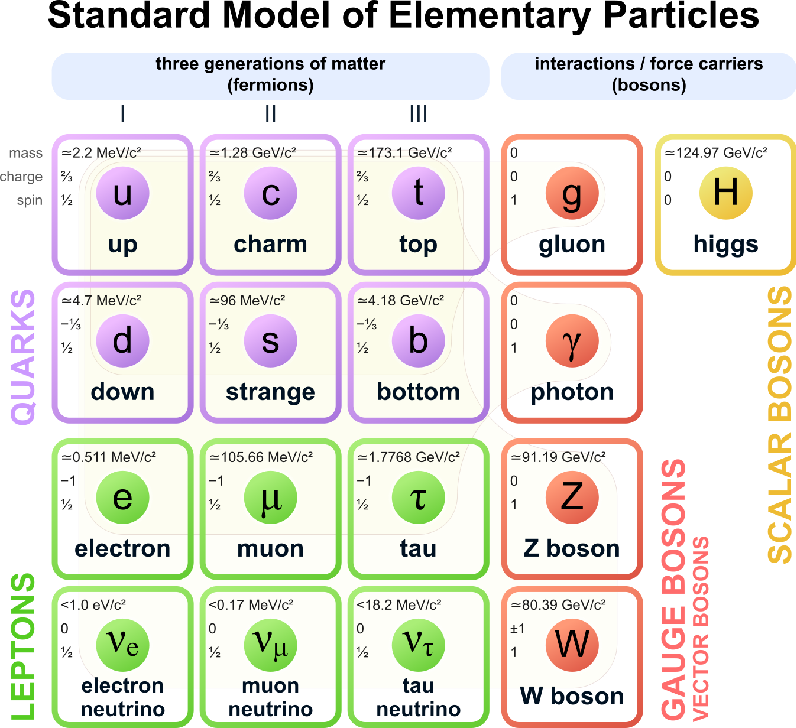
\includegraphics[width=0.7\textwidth]{Figures/1/StandardModel.pdf}
	\caption[]{Names and fundamental properties of particles in the Standard Model. Figure from \(\copyright\) \cite{sm_graphic}.}
	\label{fig:standard_model}
\end{figure}

\subsection{Fermions}
\label{sec:fermions}

Fermions are further sub-divided into leptons and quarks, depending on the charges they carry, and hence by the forces with which they interact. There are three known generations of fermions, labelled I, II and III in Figure \ref{fig:standard_model}, each with significantly larger mass than the last. Each generation contains a pair of quarks and a pair of leptons, along with their associated antiparticles. The quark pair consists of one ``up-type" quark with positive electric charge and one ``down-type" with negative charge. The lepton pair consists of one charged lepton and one charge-neutral ``neutrino". 

Leptons carry electric charge and weak isospin, and as a result interact with one another and with other particles carrying these charges via the EM and weak forces, respectively.  

Like leptons, quarks also carry electric charge and weak isospin, and additionally carry colour charge. The colour charge allows quarks to interact via the strong force. As a result, quarks interact by all three forces described by the SM. Unlike charged leptons, which carry an electric charge of \(\pm1\), quarks carry fractional electric charge; up-type (down-type) quarks carry a charge of \(+\frac{2}{3}\) \(\big(-\frac{1}{3}\big)\).

Due to an effect known as ``colour confinement", quarks cannot exist as stable particles in isolation, and must instead combine with other quarks to form stable ``colour-neutral" states called ``hadrons". The two major forms of hadrons are ``mesons" formed by a quark-antiquark pair and ``baryons" formed by three quarks. Although the intrinsic strength (i.e. probability) with which particles couple via the strong interaction is 3 (14) orders of magnitude greater than via the EM (weak) interaction \cite{griffiths_2008}, the range of strong force interactions is limited by colour confinement to the approximate size of the proton (\(10^{-15}\)m). The LHC collides protons with sufficient energy to probe interactions between their constituent quarks and gluons at length scales smaller than the size of the proton. Due to the large strong force coupling at this scale, there is a relatively high probability that the interactions initiated by these collisions will proceed via the strong force compared with other forces. 
%As a result, the vast majority of decay products observed in the ATLAS detector are cascades of hadronic interactions in the calorimeter referred to as ``jets" \footnote{See Section \ref{sec:had_calo} for a more detailed discussion of jets in the hadronic calorimeter.} which are initiated by hadrons produced in the collisons.

\subsection{Bosons}

Bosons in the SM are divided into ``gauge bosons" and ``scalar bosons". The gauge bosons are spin 1 force carriers that mediate interactions between particles. The photon mediates EM interactions between electrically charged particles. The gluon mediates the strong interaction between quarks. Unlike charge-neutral photons, the gluon itself carries colour charge, which allows it to self-interact via the strong force. The weak force is mediated by three particles: the electrically neutral Z boson, and two W bosons (W$^\pm$) with opposite electric charges of $\pm$1. 

Scalar bosons are defined as spin 0 particles. There is only one scalar boson in the SM, namely the Higgs boson (or, simply, the ``Higgs") \cite{HiggsTheory1,HiggsTheory2,HiggsTheory3} . Particles in the SM acquire mass via their interaction with the Higgs field. As such, the Higgs only interacts with massive SM particles, which includes all particles except the photon and the gluon. The more massive the particle, the stronger its coupling with the Higgs. Neutrinos are a possible exception; there is at present no mechanism in the SM by which neutrinos could interact with the Higgs field, so the origin of their tiny masses remains an open question.  


\subsection{Collision and Decay Processes at Colliders}
\label{sec:col_decay_procs}

The high-energy counter-rotating proton beams at the LHC are brought into head-on collisions at four interaction points around the ring, each of which is surrounded by a detector\footnote{See Chapter \ref{chapter:lhc_atlas} for a detailed discussion of the LHC and the detectors that surround the four interaction points.}. At each interaction point, constituents of the colliding protons known as ``partons"\footnote{See Section \ref{sec:parton_model} for an introduction to the parton model.} can pair annihilate to form observable collision products via one or more ``virtual mediators"\footnote{See Section \ref{sec:virtual_particles} for a discussion of virtual particles.}, and the collision products are subsequently measured by the detector. 

Each process that describes a physically allowed mechanism by which partons may annihilate to form observable particles has a certain probability of taking place relative to other possible annihilation and production processes. The probability that a given process will take place is quantified by its ``cross section" \(\sigma\). The beam luminosity \(\mathcal{L}\) relates the rate of collisions \(\frac{dN}{dt}\) that proceed via a given process to the cross section of the process:

\begin{equation}
\frac{dN}{dt} = \mathcal{L}\sigma
\end{equation}

The luminosity can be integrated over a period of time \(t_1\) to \(t_2\), such that the total number of events expected to be produced via a process with cross section \(\sigma\) over the given period is related to the ``integrated luminosity" \(\mathcal{L}_\text{int}\) by:

\begin{equation}
\label{eq:integrated_lumi}
N = \sigma\int_{t_1}^{t_2}\mathcal{L}(t)dt = \sigma\mathcal{L}_\text{int}
\end{equation}

\subsection{Unstable Particles}

The lowest-mass ``first-generation" quarks and charged leptons located in column I in Figure \ref{fig:standard_model} are, along with neutrinos and the massless photons and gluons, the only stable particles in the SM. All other particles are unstable, and will decay to less-massive particles after they are produced. 

The decay of an unstable particle occurs randomly with respect to the time elapsed since the particle was produced, with the elapsed time governed by Poisson statistics. The probability \(P(t)\) that an unstable particle will have decayed after a time \(t\) has elapsed in its rest frame is given by the following cumulative exponential distribution:

\begin{equation}
\label{eq:particle_decay}
P(t) = 1-e^{-\frac{t}{\tau}} % = e^{-\Gamma t}
\end{equation}

\noindent where \(\tau\) is the mean lifetime of the particle.

%\noindent where the decay rate \(\Gamma\) is the inverse of the mean lifetime.  

\subsubsection{Unstable Resonance and the Breit-Wigner Formula}

Due to their finite lifetime, the Heisenberg uncertainty principle implies that unstable particles will not be produced with a well-defined mass, but rather with a mass distribution peaked at a central value \(m_0\). The probability density function \(p(m)\) associated with measuring an unstable particle to have a mass \(m\) is given by the Breit-Wigner formula \cite{breit_wigner}:

\begin{equation}
\label{eq:breit_wigner}
p(m) \propto \frac{1}{(m-m_0)^2 + \frac{\Gamma_E^2}{4}}
\end{equation}

\noindent which exhibits a resonant peak of width \(\Gamma_E\) centred at \(m_0\). The lifetime of the unstable particle is related to the width of its Breit-Wigner resonance by \(\tau = \frac{\hbar}{\Gamma_E}\).

For unstable mediators produced in high-energy colliders which decay to a pair of detectable particles, the mediator mass can be reconstructed as the combined invariant mass\footnote{The invariant mass \(m\) of two particles with four-momenta \(p_1\) and \(p_2\) is in general given by: \(m^2 = (p_1 + p_2)^2 = (E_1+E_2)^2 - (\mathbf{p}_1+\mathbf{p}_2)^2\)} of its measured decay products. Neglecting detector resolution effects, the cross section \(\sigma(m)\) associated with producing an unstable particle with a given reconstructed mass is expected to be proportional to its Breit-Wigner distribution: \(\sigma(m)\propto p(m)\). This results in a characteristic resonant peak in the reconstructed invariant mass distribution of the mediator's decay products, which can be used to identify the unstable mediator, and to measure its mass and lifetime.

\subsection{Feynman Diagrams}

The interaction mechanisms by which observable collision products are produced from the annihilation of two partons can be represented by Feynman diagrams, which are described in detail in Chapter 2 of Ref. \cite{griffiths_2008} and summarized here. As an example, the Feynman diagram for the Drell Yan process in which a \(q\bar{q}\) pair annihilate to form a lepton pair \(\ell\bar{\ell}\) via the exchange of a virtual photon (\(\gamma^{*}\))\footnote{The \(^{*}\) indicates that mass of the virtual particle may be off-shell (see discussion of virtual particles below).} or \(Z^{*}\) boson mediator is shown in Figure \ref{fig:drell_yan}. 

The particles involved in the interactions are represented as lines in a Feynman diagram, with different particle types represented by different line styles - fermions are generally represented by solid straight lines, and bosons (with the exception of gluons) are generally represented by wavy lines. Particle interactions are represented by vertices at which lines in the diagram intersect. The annihilation of a \(q\bar{q}\) pair to form the virtual \(\gamma^{*}/Z^{*}\) mediator is represented in Figure \ref{fig:drell_yan} by the vertex at which the \(q\) and \(\bar{q}\) fermion lines meet the \(\gamma^{*}/Z^{*}\) boson line, and the subsequent decay of the  \(\gamma^{*}/Z^{*}\) to \(\ell\bar{\ell}\) is represented by the vertex to the right at which the \(\gamma^{*}/Z^{*}\) line meets the \(\ell\) and \(\bar{\ell}\) lines. Note that time flows horizontally from left to right in Feynman diagrams, so the colliding \(q\bar{q}\) pair are shown on the left and the observable decay products \(\ell\bar{\ell}\) on the right.

\begin{figure}[h]
	\centering
%	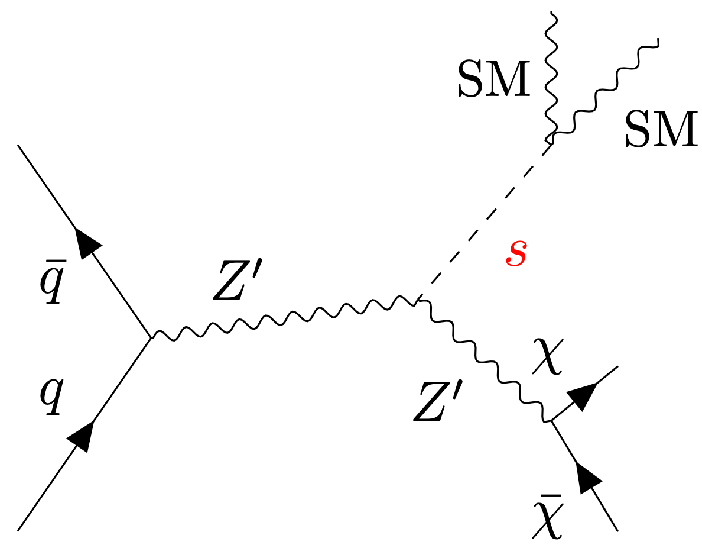
\includegraphics[width=0.95\textwidth]{Figures/2/Fey1.pdf}
		\begin{tikzpicture}
			\begin{feynman}

		 		\vertex (a1);
		 		\vertex at ($(a1) + (0cm, -3cm)$) (b1);
		 		\vertex at ($(a1) + (1cm, -1.5cm)$) (c1); %gamma/Z
		 		\vertex at ($(c1) + (2cm, 0cm)$) (c2); %gamma/Z
				\vertex at ($(c2) + (1cm, -1.5cm)$) (d1);
				\vertex at ($(c2) + (1cm, 1.5cm)$) (d2);

		 		\diagram* {
		 		  {[edges=fermion]
		 		    (b1) -- [edge label=\(q\)]( c1) -- [edge label=\(\bar{q}\)](a1),
				    (d1) -- [edge label=\(\bar{\ell}\)]( c2) -- [edge label=\(\bar{\ell}\)](d2),
		 		  },
		 		  (c1) -- [boson, edge label=\(\gamma^{*}/Z^{*}\)] (c2),
		 		};
		 	\end{feynman}
		 \end{tikzpicture}
	\caption{Feynman diagram for the Drell Yan process.}
	\label{fig:drell_yan}
\end{figure}

\subsubsection{Virtual Particles}
\label{sec:virtual_particles}

In general, ingoing and outgoing lines in a Feynman diagram represent real observable particles, and internal lines represent so-called virtual particles. Virtual particles are not observable, but are rather a representation of the mechanism involved with producing the observable final-state particles. Importantly, virtual particles can take on any mass needed to satisfy energy and momentum conservation at each interaction vertex.
% with which they are involved. 
% are not in general produced with the mass of their corresponding real particle, but can in principle take on whatever mass is needed to satisfy energy and momentum conservation at each interaction vertex that they are involved with. 

\subsubsection{Matrix Element}

%In order to study collision events measured by particle detectors at the LHC, it is important to calculate the rate at which the detector would be expected to measure collision events which proceed by different processes, such as the Drell-Yan process shown in Figure \ref{fig:drell_yan}. 

The final-state observables (momenta of outgoing particles) associated with a process of particle production from \(pp\) collisions at the LHC, such as the Drell-Yan process shown in Figure \ref{fig:drell_yan}, depend in general on both the phase space and dynamics of the process. The phase space represents the full space of available kinematics (masses and momenta) for the incoming and outgoing particles. The dynamics are encoded in the matrix element \(\mathcal{M}\), which is calculated on the basis of the internal structure of the process as represented by the Feynman diagram. 
%The matrix element the coupling constants which quantify the interaction strength of the particles involved at each interaction vertex and an integration over the possible dynamics of the virtual particles. 

%kinematic available masses and momenta of the incoming and outgoing particles. The dynamical information is enc
%
%general proportional to an integral of the squared matrix element \(|\mathcal{M(\boldsymbol{x}, \boldsymbol{\alpha})}|^2\):
%
%\begin{equation}
%\label{eq:matrix_element}
%\sigma \propto \int|\mathcal{M(\boldsymbol{x}, \boldsymbol{\alpha})}|^2 d\boldsymbol{x} 
%\end{equation}
%
%
%
%\noindent where the quantities \(\boldsymbol{x}\) describe the dynamics (masses, momenta, quantum numbers, etc.) of the incoming and outgoing observable particles, and \(\boldsymbol{\alpha}\) are terms which describe the internal structure of the process represented by the Feynman diagram, including the coupling constants which quantify the interaction strength of the particles involved at each interaction vertex and an integration over the possible dynamics of the virtual particles. 

\subsection{Mathematical Formulation of the Standard Model}
\label{sec:sm_math}

The SM is formulated mathematically as a quantum field theory, in which particles of the SM are represented as excitations of quantum fields. The mathematical formulation of the SM is presented in detail in standard texts \cite{griffiths_2008, SM_intro}, and briefly summarized in this section, with focus placed on aspects that are relevant to later discussions in this thesis.

\subsubsection{Lagrangian Densities}

As in classical field theories, the quantum fields of the SM and their interactions are powerfully described by the formalism of Lagrangian densities, which are functions of the quantum fields and their derivatives. For example, interactions between photons and electrically charged fermions are described in quantum electrodynamics (QED) by the following Lagrangian density term:

\begin{equation}
\label{eq:qed_interaction}
\mathcal{L}_\text{QED, interaction} = -q\psi^\dagger(x)\gamma^0\gamma^\mu\psi(x) A_\mu(x)
\end{equation}

\noindent where \(\psi(x)\), a function of the four spacetime coordinates represented by \(x\), is the quantum spinor field of the spin-\(\frac{1}{2}\) fermions in the SM. \(A_\mu(x)\) represents the vector field of the massless spin-1 photon and \(\gamma^\mu\) are the Dirac matrices \cite{griffiths_2008}. The index \(\mu\) runs over the four spacetime coordinates. The factor \(q\) represents the electric charge of the fermion involved in the interaction and its value\footnote{The electric charges of all fermions in the SM are as follows: \(\pm1\) for charged leptons, \(+\frac{2}{3}\) (\(-\frac{1}{3}\)) for up (down) type quarks and 0 for neutrinos.} determines the strength of the interaction. 

\subsubsection{Symmetries and Groups Theory Description}

Symmetries in the Lagrangian density function associated with each fundamental interaction are described in the language of group theory by classifying the fundamental interactions into gauge groups that describe their symmetries. For example, QED exhibits a symmetry under local phase transformations, described by the unitary local gauge group U(1). This means that the Lagrangian \(\mathcal{L}_\text{QED}\) is invariant under the multiplication of the fermion spinor \(\psi(x)\) by a unitary function \(U = e^{i\theta(x)}\) (unitarity implies that \(U^\dagger U=1\)),
%, which represents a local phase transformation 
where \(\theta(x)\) can be any function of the spacetime coordinates \(x\). It is found that this symmetry can be ensured by the inclusion of the vector field \(A_\mu(x)\) in the QED Lagrangian, which is identified with the physical photon. Because it ensures invariance under the U(1) gauge group, the vector field \(A_\mu(x)\) is referred to as a ``gauge field", and the corresponding boson (the photon) as a ``gauge boson". The symmetries in the SM are described by the direct product\footnote{General definitions in group theory can be found, for example, in Section 1.1 of Ref. \cite{costa2012symmetries}.} of the U(1)\(\times\)SU(2)\(\times\)SU(3) gauge groups. 

\subsubsection{Quantum Chromodynamics}

The theory of quantum chromodynamics (QCD), presented in standard texts such as Ref. \cite{qcd_2007}, describes the strong interactions mediated by gluons between particles with colour charge (quarks and gluons). Its symmetries are described by the SU(3) gauge group. The quarks are represented by a three-component vector of spinors: \(\psi_c = \{\psi_r, \psi_g, \psi_b\}\), where the subscripts refer to the three colours - red, green and blue - that constitute the charges of the strong interaction. The QCD Lagrangian (see eg. Eq. 10.88 in Ref. \cite{griffiths_2008}) is symmetric under a transformation of the vector of quark spinors \(\psi_c\) by a \(3\times3\) SU(3) matrix, which is unitary with determinant 1. The SU(3) symmetry is ensured by the inclusion of an eight-component set \(\boldsymbol{\boldsymbol{A}_\mu}\) of vector gauge fields in the QCD Lagrangian. The associated gauge bosons are identified as the eight physical gluons, each of which possesses a unique superposition of \({rgb}\) colour states \cite{griffiths_2008}.

\subsubsection{Electoweak Theory and the Higgs Mechanism}

The mathematical descriptions of the weak and EM forces are unified into a single ``electroweak" theory (for a review, see \cite{electroweak_2012}) whose symmetries are described by the SU(2)\(\times\)U(1) product of gauge groups. 

Developed in 1954, Yang-Mills theory \cite{yang_mills_1954} showed that a set of three vector gauge bosons, referred to as the ``isospin triplet" \(\boldsymbol{W}\) are needed to satisfy the SU(2) symmetry, and a fourth massless vector gauge boson \(B\) is needed to satisfy the U(1) symmetry. Despite satisfying the SU(2) symmetry of the weak interaction, the weak isospin triplet predicted by Yang-Mills theory falls short of fully describing the physical \(W^{\pm}\) and \(Z\) bosons that mediate the weak interaction, which are known to be massive \cite{pdg_2020}.

The U(1)\(\times\)SU(2)\(\times\)SU(3) symmetry of the SM Lagrangian does not admit mass terms of the form \(m_X^2X^\dagger X\), where X is an arbitrary field. Proposed in 1964, the ``Higgs mechanism" \cite{HiggsTheory1,HiggsTheory2,HiggsTheory3} provides a means of generating the masses of the physical \(W^\pm\) and \(Z\) bosons, as well as all other massive particles (with the exception of neutrinos), by adding the following term to the SM Lagrangian:

\begin{equation}
\label{eq:higgs_lagrangian}
\mathcal{L}_\text{Higgs} = (D^\mu H)^\dagger(D_\mu H) - V(H)
\end{equation}

\noindent where

\begin{equation}
H = \frac{1}{\sqrt{2}}
\begin{pmatrix}
0 \\
h+v
\end{pmatrix}
\end{equation}

 \(h(x)\) is interpreted as the scalar field of the physical Higgs boson, and \(v\) as the so-called ``vacuum expectation value". With \(H\) in this form, \(\mathcal{L}_\text{Higgs}\) is described by the U(1) symmetry group but not the SU(2) group, and is thus said to ``break" the electroweak symmetry SU(2)\(\times\)U(1) to the QED gauge symmetry U(1).

The covariant derivative \(D_\mu H\) in Eq. \ref{eq:higgs_lagrangian} takes the form:

\begin{equation}
\label{eq:D_muH}
D_\mu H = \big(\partial_\mu + i\frac{1}{2}g\sigma_k W^k_\mu+i\frac{1}{2}g'B_\mu\big)H
\end{equation}

\noindent where \(\sigma_k\) are the Pauli matrices, and \(g\) and \(g'\) are the coupling constants between the Higgs field and the \(\boldsymbol{W}\) and \(\boldsymbol{B}\) fields, respectively.

The Higgs potential \(V(H)\) takes the form:

\begin{equation}
V(H) = -\mu^2H^\dagger H + \lambda(H^\dagger H)^2
\end{equation}

\noindent where the second term describes quartic self-interactions of the Higgs field.

The emergence of the massive physical \(W^\pm\), \(Z\) bosons and the massless photon comes from the interactions of the electroweak \(\boldsymbol{W}\) and \(B\) fields with the Higgs field to produce ``mass" terms in the Lagrangian of the form \(m_X^2X^\dagger X\). This can be seen by expanding Equations \ref{eq:higgs_lagrangian} and  \ref{eq:D_muH}, considering only the terms involving the vacuum expectation value \(v\):

\begin{equation}
\label{eq:higgs_expanded}
\mathcal{L}_\text{Higgs} = \frac{v^2}{8}\Big[g^2\big((W^1_\mu)^2+(W_mu^2)^2\big) + (gW^3_\mu-g'B_\mu)^2\Big] + [...]
\end{equation}

\noindent with the physical vector boson fields and masses defined as:

\begin{equation}
\label{eq:physical_v_bosons}
\begin{split}
W^\pm_\mu & \equiv \frac{1}{2}(W_\mu^1 \mp W_\mu^2) \phantom{xxxxxxxxxlxx}\text{ with mass }\phantom{xxx} m_W=\frac{gv}{2} \\
Z_\mu & \equiv \frac{1}{\sqrt{g^2+g'^2}}(gW_\mu^3-g'B_\mu) \phantom{xxx}\text{ with mass }\phantom{xxx} m_Z = \frac{v}{2}\sqrt{g^2+g'^2} \\
A_\mu & \equiv \frac{1}{\sqrt{g^2+g'^2}}(g'W^3_\mu+gB_\mu) \phantom{xxx}\text{ with mass }\phantom{xxx} m_A = 0
\end{split}
\end{equation}

Inserting the definitions of the physical vector boson fields from Eq. \ref{eq:physical_v_bosons} back into Eq. \ref{eq:higgs_expanded}, it can be readily confirmed that Eq. \ref{eq:higgs_expanded} takes the form \(\mathcal{L}_\text{Higgs} = \big[(W^\pm)_\mu^\dagger(W^\pm)^\mu + Z_\mu^\dagger Z^\mu + A_\mu^\dagger A^\mu\big] + [...]\). Masses of fermions are likewise generated by so-called Yukawa couplings \cite{weinberg_1967} between the fermion and Higgs fields. The dark Higgs model used to optimize and interpret the DM search presented in this thesis postulates that DM, as well as any hypothetical new bosons that mediate its interactions with SM particles, would acquire their masses by means of their interaction with the dark Higgs field \(S\), as discussed in Chapter \ref{chapter:dh_model}. 


\section{Evidence for Dark Matter from Observational Astronomy}

Looking beyond the SM, many independent astronomical observations collectively provide compelling evidence for the presence and abundance of a new form of matter in the universe that is not directly observable because it neither emits nor absorbs light. Some of the earliest and clearest evidence for this so-called ``dark matter" (DM) came in 1978, when Rubin et al. \cite{Rubin_et_al} reported systematic anomalies in measured rotation speeds of spiral galaxies. In particular, distributions of the rotation speed as a function of the radial distance from the galactic centre differed in shape from what would be expected on the basis of the distribution of galactic mass measured from the observed luminosity profile. 

\begin{figure}[H]
	\centering
	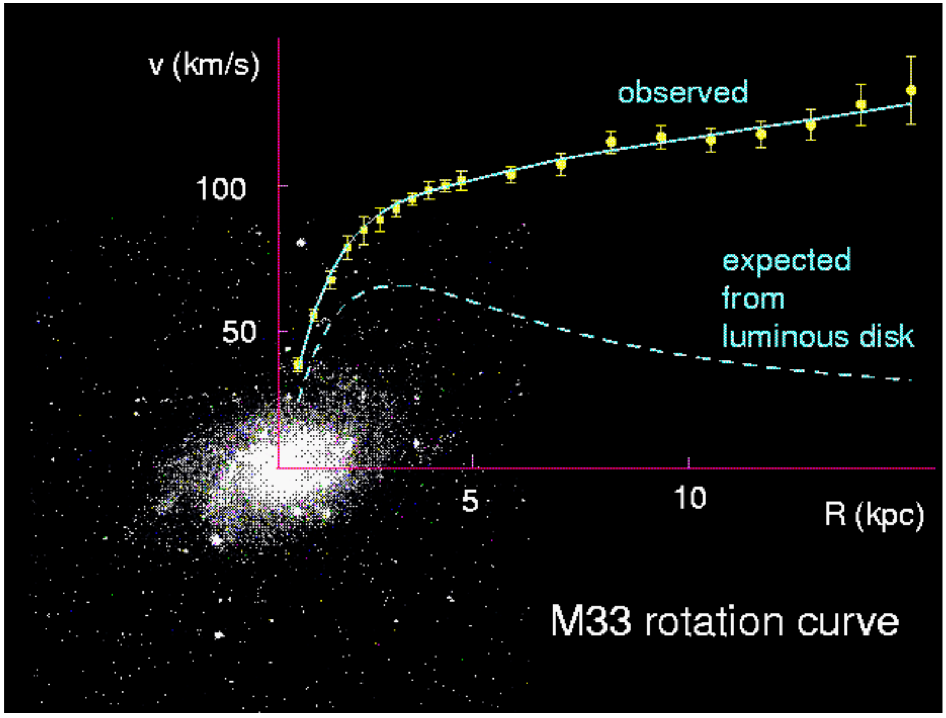
\includegraphics[width=0.6\textwidth]{Figures/1/m33_rotation.pdf}
	\caption[]{Observed rotation speed of the nearby dwarf galaxy M33, overlaid on an optical image of the galaxy. Yellow data points show observed rotational speed of the galaxy as a function of the radial distance from the galactic centre (in kpc). Dashed line shows the expected rotational speed on the basis of the calculated mass of the luminous stellar disk. Figure from \(\copyright\) \cite{m33_2000}.}
	\label{fig:m33_rotation}
\end{figure}

Spiral galaxies were known at the time to be comprised of a central spheroidal ``galaxy bulge" that contains the majority of luminous matter in the galaxy, in addition to a ``disk" extending out to larger radii from the galactic centre, within which the density of luminous matter falls off exponentially with radius. If one assumes that the distribution of mass in the spiral galaxy follows its luminosity profile, application of Newtonian gravitational mechanics\footnote{Rotation speeds of spiral galaxies are in general non-relativistic (typically \(v_\text{rot}/c<1\%\) \cite{rotn_curves_1995}). Since Newtonian gravitational mechanics represents an accurate approximation of general relativity in this macroscopic non-relativistic regime, it is generally assumed to provide an appropriate framework for the mathematical description of galactic rotation curves.} would predict the rotation speed to peak near the edge of the central galaxy bulge, as illustrated in the blue dashed line in Figure \ref{fig:m33_rotation} for the dwarf galaxy M33, and fall off at larger radii due to the exponentially decaying matter density of the disk. However, the observed galactic rotation speed, shown as yellow data points in Figure \ref{fig:m33_rotation}, is generally observed to continue increasing well beyond the luminous galactic bulge. These anomalies in galactic rotation curves, which have since been observed in hundreds of spiral galaxies \cite{rotn_curves_1995}, can be explained by postulating an additional source of non-luminous matter density in galaxies, DM, which extends well beyond the luminous bulge and provides the necessary gravitational potential to prevent the rotation speeds from falling off beyond the bulge.

In the years following the early reports by Rubin et al., modifications to the laws of Newtonian gravity at galactic scales \cite{mond_1983} were considered as an alternative to explain the anomalies without invoking the need for DM. However, while the proposed modifications to gravity were successful in describing the observed galactic rotation curves, numerous astronomical observations in other contexts have independently turned up results that indicate a need for DM in the universe, many of which cannot be easily explained by modifying Newtonian gravity. Additional evidence at galactic scales comes from significant differences between the spatial distributions of matter density, measured using gravitational lensing, and of luminous matter following collisions of galaxy clusters, such as the Bullet cluster identified in 1995 \cite{bullet_1995}, which indicate that the majority of the matter density in the colliding galaxies is non-luminous. Studies of the relative contribution to the masses of galaxy clusters from luminous matter using data from the Chandra X-ray observatory \cite{Chandra_2013} suggest that only 15-20\% of the mass composition of the galaxies studied is comprised of luminous matter, with DM comprising the remaining 80-85\%.

Because of their stability and EM interactions, protons and neutrons comprised of bound quarks, as well as their bound electrons - collectively known as ``baryonic matter" - comprise by mass the overwhelming majority of known luminous matter in the universe. The theory of Big Bang nucleosynthesis (BBN) (for a review, see Section 24 of Ref. \cite{pdg_2020}) predicts that the production of light nuclei - D, \(^2\)He, \(^4\)He, and \(^7\)Li - took place in the early universe following the Big Bang (see Ref. \cite{uzan2016bigbang} for a review of the Big Bang theory), as the universe expanded and cooled sufficiently to allow their formation by means of nuclear fusion reactions. BBN theory predicts that the abundances of these light nuclei in the universe were fixed during BBN, following which the rate of the nuclear fusion reactions became negligibly small due to the continued expansion and cooling of the universe. Importantly, the theory also predicts that the relative abundances of the light nuclei are highly sensitive to the density of baryonic matter in the universe, which was fixed prior to their formation. As a result, their relative abundance can be used to infer the density of baryonic matter in the universe in the context of BBN theory. Using this approach, precision measurements of the abundances of light nuclei inferred from observational data indicate that baryonic matter constitutes approximately 5\% \cite{pdg_2020} of the energy density of the universe. Current measurements of anisotropies in the cosmic microwave background (CMB) \cite{cmb_1965} measured by the Planck collaboration \cite{Planck_2020}, interpreted in the context of the \(\Lambda\)CDM model of cosmology (for a review, see Section 25 of \cite{pdg_2020}), indicate that approximately 30\% of the energy density of the universe is comprised of matter, with the missing 25\% identified as non-baryonic DM. This result implies that \(~85\%\) of all matter in the universe is comprised of non-luminous DM, consistent with the findings discussed above from measurements of galaxy clusters.

\section{Dark Matter Composition Hypotheses}

The previous section presented a diverse range of astronomical observations that collectively point to the need for DM in the universe. While active research continues within the theoretical community (see, for example, Refs. \cite{mond_2012, mond_2021}) into the possibility of modifying the laws of gravitation at astronomical scales to explain these observations without the need for DM, there are significant theoretical challenges involved with designing modifications that can consistently explain the range of observational anomalies at scales ranging from individual galaxies to galaxy clusters, while simultaneously addressing the apparent need for DM at cosmological scales from the discrepancy between measurements of the baryonic mass density from BBN and the much larger total mass density inferred from anisotropies in the CMB. As a result, DM is widely considered the leading hypothesis to explain the full range of observational data.

While the astronomical observations provide a wealth of information regarding the composition of DM in the universe by means of its gravitational effects on visible matter, they provide relatively few clues as to what actually comprises the DM. Its abundance in the present day universe indicates that it must be stable on cosmological timescales (i.e. billions of years). The evidence from BBN and CMB anisotropies indicates that the DM must be non-baryonic. Its non-luminous nature further implies that it neither emits nor absorbs photons, and therefore has negligible or no charge under the EM force. Besides baryons, neutrinos - with their tiny but nonzero masses\footnote{Current constraints from cosmology place an upper limit on the sum of neutrino masses from all generations of 0.17 eV, \(~3\times10^6\) times smaller than the electron mass.} - represent the only other massive stable particles currently known to the SM, and satisfy the requirement of being electrically neutral. However, the possibility of neutrinos constituting any appreciable fraction of the DM was ruled out by studies published in the 1980's \cite{neutrino_dm}, which demonstrated that the large scale structure of the universe would differ significantly from what is observed today if the mass density of the universe were dominated by neutrinos due to their ultra-relativistic velocity. More generally, analysis of the measured anisotropies in the CMB measured by the Planck collaboration \cite{Planck_2020} is found to strongly favour the standard \(\Lambda\)CDM model in which the DM is predominantly comprised of ``cold" particles, so called because they travel at non-relativistic velocities.

With the stable particles of the SM ruled out, the current most widely accepted hypothesis is that DM is comprised of a new form of cold non-baryonic matter that is not currently described by the SM.

\subsection{Origin and Interactions of Particle Dark Matter}
\label{sec:dm_origins}

Despite the observable effects of its gravitational interactions at astronomical scales, the strength of gravitational couplings between massive particles is \(\sim30\) orders of magnitude weaker than any of the other three known forces \cite{griffiths_2008}. As a result, gravitational interactions between DM and SM particles are far too weak to be observable in particle detectors. Given that there have not yet been any conclusive indications of DM in particle detectors, it can be further deduced that any non-gravitational interactions between DM and particles of the SM are relatively weak compared with the strong, weak and EM couplings between SM particles. However, most theories that aim to describe the origin of the observed abundance of DM in the present day universe imply the existence of non-gravitational couplings between DM and SM particles, and in many cases predict that the couplings could be strong enough to be probed by modern particle detection methods. This produces a generic class of DM candidates known as weakly-interacting\footnote{The ``weak" interactions of the WIMP DM candidates are in general not necessarily associated with the weak force, but are simply too weak to have produced a measurable signature in particle detectors to date} massive particles (WIMPs). 
%The strength of the WIMP hypothesis has inspired worldwide efforts spanning several decades to design increasingly sensitive particle detectors and targeted studies to detect evidence of WIMPs. Such a detection would not only confirm the WIMP hypothesis,

A positive detection of WIMPs would not only confirm the hypothesis of particle DM, but would also allow physicists to begin to study its properties as a particle, and test theoretical extensions of the SM that incorporate particle DM.

\subsubsection{Dark Matter Origin from Thermal Freeze-out}

A review of the existing hypotheses for the origin of DM can be found in Section 27.3 of Ref. \cite{pdg_2020}. Of these, the so-called ``thermal freeze-out" scenario is a popular candidate, because it postulates that the observed DM density in the present day universe originated from the same process of thermal decoupling that produced the primordial abundances of light nuclei in the well-tested BBN scenario discussed earlier. The hypothesis postulates that in the very early universe, matter was sufficiently dense and energetic to establish thermal equilibrium between DM and SM particles due to interactions between DM and SM particles (so-called ``DM-SM interactions"). As the universe expanded and cooled, eventually the rate of DM-SM interactions became too low to maintain thermal equilibrium between the two species. At this point, known as ``thermal freeze-out", DM became decoupled from SM particles, thus fixing the relic abundance of DM observed in the present-day universe. 

For cold DM relics (\(v/c\lesssim0.1\) at the time of freeze-out), and assuming that the relic abundance is predominantly set by direct DM-SM interactions, analysis of the observed relic abundance of DM in the context of the thermal freeze-out hypothesis (see, for example, Section B of Ref. \cite{dm_xsec_2015}) implies that the cross section for SM-DM interactions should be \(\sigma_\text{SM-DM}\gtrsim1\) pb, comparable to typical cross sections for interactions mediated by the weak force. Searches for DM in particle detectors (for a review, see \cite{wimp_searches_2018}) have yet to turn up any hints of a DM candidate with interaction cross sections with the SM near the weak scale. However, the cross section constraint can be significantly relaxed by considering a scenario in which the relic abundance of DM is set not by direct interactions between the DM and the SM, but rather by interactions between DM and an unstable mediator, which subsequently decays to SM particles (see, for example, Ref. \cite{secluded_dm_2008}). The DM search presented in this thesis is interpreted in the context of such a scenario, wherein the unstable mediator is the Dark Higgs boson \cite{Duerr_2016,Duerr2017}.

\section{Dark Matter Search Strategies}

There are three complementary approaches used to search for particle DM by means of its non-gravitational interactions. Direct detection searches (for a review, see \cite{billard2021direct}) aim to detect evidence of a recoil induced by elastic scattering between a DM particle in the galactic halo and a target particle in the detector. Indirect searches (for a review, see \cite{CIRELLI_2012}) use observational data to search for evidence of particles produced by DM annihilation or decay in particular regions of the observable universe that are expected to have a high DM density. Searches for DM at colliders (for a review, see \cite{DM_colliders}), of which the work in this thesis is an example, study the decay products from high-energy collisions of subatomic particles to search for an above-background excess of events that could be consistent with DM having been produced in some of the collisions.

\subsection{Direct Detection}

Direct detection searches operate in very low-background environments, typically in underground facilities such as SNOLAB (for a review, see Ref. \cite{Lawson_2013}), in order to minimize scattering events in the detectors from non-DM sources such as cosmic rays and radioactivity, and detailed studies are performed to determine the expected rate of events from all possible background sources. As a result, a significant excess of elastic scattering events, particularly if observed in multiple direct detection experiments, would offer a clear signature of interactions with DM in the galactic halo. 

If no evidence of excess scattering events is found, experiments place upper bounds on DM-nucleon interaction cross section with a largely standard set of methods and assumptions (most notably the local DM density and the relative speed with which the DM passes through Earth) (see, for example, Ref. \cite{dd_results_standards_2021}), which facilitates comparison between different experiments. Figure \ref{fig:dd_limits} summarizes the current upper bounds on the spin-independent\footnote{Spin-dependent vs. spin-independent DM-nucleon interactions differ according to whether the coupling is sensitive to the spin state of the target nucleon \cite{billard2021direct}.} DM-nucleon interaction cross section from all direct detection searches. The searches probe down to many orders of magnitude below the weak scale (\(\sigma\sim10^{-36}\)cm\(^{-2}\)) over \(\sim4\) orders of magnitude of candidate DM masses. However, current direct detection strategies generally suffer practical limitations to the ranges of DM masses and interaction cross sections that can be probed. The lower bound on accessible DM masses is in general dictated by the signal to noise ratio of the detector, referred to as the ``noise wall", which is quite difficult to overcome. The range of accessible cross sections is also bounded from below for most direct detection experiments by the so-called ``solar neutrino floor", below which the measured event rate becomes dominated by the irreducible flux of solar neutrinos passing through the Earth. 

\begin{figure}[h]
	\centering
	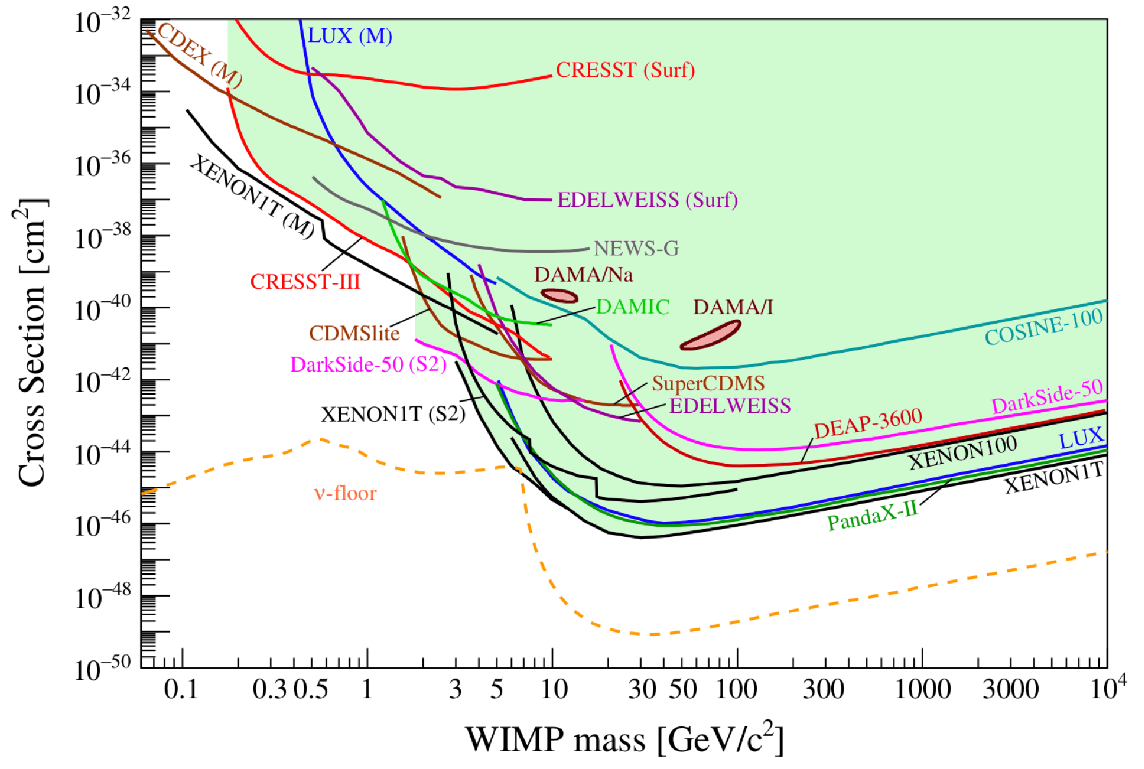
\includegraphics[width=0.7\textwidth]{Figures/1/dd_results.pdf}
	\caption[]{Summary of upper bounds from direct detection searches on the interaction cross section for spin-independent WIMP-nucleon scattering, over a range of hypothetical WIMP masses. Upper bounds from individual searches are shown as solid lines. Results labelled ``M" were obtained assuming the Migdal effect \cite{migdal_2018}. Shaded green region shows combined exclusion from all searches, excluding results obtained assuming the Migdal effect. Yellow dashed line shows the solar neutrino floor for a Ge target, computed using the assumptions and methodology presented in Refs. \cite{neutrino_floor_1, neutrino_floor_2}. Figure from \(\copyright\) \cite{billard2021direct}.}
	\label{fig:dd_limits}
\end{figure}

\subsection{Indirect Detection}

By searching for excesses of several potential DM annihilation products in observational data - gamma rays and charged leptons and antimatter - in addition to neutrinos, indirect detection searches (reviewed in Refs. \cite{CIRELLI_2012,conrad2014indirect, pdg_2020}) can avoid the limitation of the solar neutrino floor. Depending on the target species, these searches can also target a wider range of candidate DM masses compared with direct detection searches. Due to the many potential processes that could produce the target particles in observational data - both within and beyond the SM - indirect searches generally contend with relatively large uncertainties associated with modelling the expected flux from these background sources. 
%Indirect searches generally probe \(\langle \sigma v \rangle\), where \(\sigma\) is the the DM-DM annihilation cross section, \(v\) is the velocity of the target DM relative to Earth, and the average represented by \(\langle\rangle\) is over the expected distribution of \(v\) as a function of the DM mass, for an assumed DM density in the target region. 

\subsection{Searches for DM at Colliders}

Rather than searching for non-gravitational interactions of relic DM on Earth or in the observable universe, searches for DM at colliders (for a review, see \cite{DM_colliders}) instead look for evidence of DM production from high-energy particle collisions. Like neutrinos, DM would be expected to pass invisibly through any detector surrounding the collision point due to its very low interaction cross section, producing a momentum imbalance transverse to the beam line referred to as \met\footnote{See Section \ref{sec:met} for a detailed introduction to missing transverse momentum in the ATLAS detector.}. An excess of collision events with large final-state \met above the rate expected from SM processes with final-state neutrinos would be consistent with the production of DM in the high-energy collisions. Given that other hypothetical new physics processes (see, for example, Refs. \cite{add_1998, dark_energy_lhc}) could also produce an excess of high-\met events from non-DM sources, any such findings would benefit from corroborating DM detections in direct and/or indirect detection experiments.

Despite operating in a very high background environment, colliders offer numerous advantages that allow DM searches performed using collider data to complement and potentially extend the reach of direct and indirect searches. First, the detectors used by particle colliders are often designed to measure all final-state particles produced by the collisions and their kinematic information with high precision. This detailed final-state information allows DM searches to target specific final-state topologies, which can lead to substantial reductions in SM background processes and considerably enhance the sensitivity to hypothetical DM production processes that predict events with the targeted topology. Second, by targeting DM produced in the collisions and adopting a search strategy that does not require the DM to interact with the detector, searches at colliders are insensitive to the neutrino floor that will challenge the sensitivity of next-generation direct detection searches. Third, while the range of DM masses is bound from above by the centre of maximum centre-of-mass energy of the particle collisions (\(\sim\)TeV for proton-proton collisions at the LHC), DM searches at colliders do not suffer the noise wall that limits the sensitivity of direct detection searches below \(\sim1~\GeV\) (see Figure \ref{fig:dd_limits}).

Even if particle DM is first discovered at a non-collider experiment, the detailed final-state information available in particle collision data will enable detailed measurements of its properties and interactions, provided that it can be produced at colliders.

\subsection{Searching for Dark Matter at Particle Accelerators}

\subsubsection{Approaches used to Search for DM at Colliders}

The concept of searching for evidence of DM production in high-energy particle collisions is currently being pursued by numerous collaborations. The particular energy scales and detector technologies available to each experiment can be exploited to target specific mass ranges and possible DM production mechanisms, thus allowing for a rich programme of complementary searches.

The proton-proton collision experiments at the Large Hadron Collider (LHC)\footnote{See Section \ref{chapter:lhc_atlas} for a general introduction to the LHC and its major detectors.} \cite{lhc_machine} - ATLAS \cite{atlas}, CMS \cite{cms} and LHCb \cite{LHCb} - benefit from the world-leading 13 TeV centre-of-mass energy of the \(pp\) collisions to probe models with massive mediators (\(m_\text{med}\) up to a few TeV) of the DM-SM interactions that could be produced in the collisions. The hermetic\footnote{Hermetic detectors, of which ATLAS and CMS are examples, are designed to detect all SM decay products from a collision with the exception of neutrinos.} coverage and precise event reconstruction available with the ATLAS and CMS general-purpose detectors make it possible to probe a wide range of hypothetical DM production models and final-state signatures, typically targeting DM candidates with masses in the \(\sim\)GeV-TeV range (see Ref. \cite{Trevisani:2018psx} for a review of DM searches performed with the ATLAS and CMS detectors). Meanwhile, DM searches at LHCb (for a review, see \cite{mombacher2021dark}) take advantage of the detector's excellent forward-angle coverage and vertex resolution to target signatures with lower-mass DM (\(\sim\)MeV-GeV) and displaced vertices.

In addition to proton-proton collisions at the LHC, production of DM in electron-positron \(e^+e^-\) collisions has been probed with the BABAR experiment \cite{babar_2002} at the Stanford Linear Accelerator Centre (SLAC), as well as the Belle experiment \cite{belle_detector_2002} and its recent Belle II upgrade \cite{belle_II_2018} at the SuperKEKB collider \cite{superkekb_2018}. With a 10.6 GeV centre-of-mass collision energy, the Belle II experiment is particularly well suited to study DM with masses in the range of a few MeV to 10 GeV. Searches at \(e^+e^-\) colliders benefit in precision both from the well-defined initial state afforded by colliding fundamental particles, and from the vastly reduced background of QCD activity\footnote{See Section \ref{sec:trigger} for a more detailed discussion of the QCD background in the context of the ATLAS triggering system.} in the final state compared with \(pp\) collision events. Searches performed with early Belle II data, reviewed in Ref. \cite{Campajola_2021}, are already showing promising sensitivity to a number of low-mass DM candidates, with significant sensitivity improvements expected as more data is collected in the coming years.

The most direct way to search for DM at \(pp\) and \(e^+e^-\) colliders is to look for evidence of the so-called ``\met+X" events introduced above, in which the DM is produced along with detectable SM particles, thus producing a signature of SM particles recoiling against \met in the final state. An alternative and less direct approach, known as a ``resonance search", is to look for evidence of the production of new massive mediators which could potentially mediate DM-SM interactions by looking for resonant peaks in the invariant mass distribution of one or more pairs of final-state particles. Such a peak, if not associated with any known SM mediators, would be indicative of the production and subsequent decay of a new massive mediator to a pair of SM particles.

DM in the \(\sim\)MeV-GeV mass range can also be probed with competitive sensitivity at fixed-target experiments in which a beam of energetic electrons or protons is directed at a fixed target, and downstream detectors search for evidence of DM produced from the electron-nucleon or proton-nucleon collisions. A variety of approaches are employed by different experiments to search for signatures of DM production. Some searches re-purpose neutrino detectors, such as MiniBooNE \cite{miniboone_2018} and NOvA \cite{nova_2017} at Fermilab, to directly detect any DM that may be produced in the collisions by means of DM-nucleon or DM-electron collisions with the detector material, placing additional shielding between the fixed target and the detector to reduce the background flux of neutrinos. Others such as NA64 \cite{na64_2019} at CERN employ a fully hermetic detector to search for a \met+X signature of DM in the downstream collision products.

\subsubsection{Models of DM Production}

Models of DM production in colliders can range in complexity from an effective field theory (EFT), where the DM production mechanism is completely unspecified, to a complete model such as supersymmetry, which predicts viable DM candidates as part of a hypothesized extension to the SM designed to address a range of phenomena unexplained by the SM (see Ref. \cite{susy_dm} for a review of supersymmetric DM candidates). 

%The EFT approach treats the production of DM from colliding partons as a contact interaction, with the production rate determined by a single parameter \cite{DM_colliders}. As long as a measurable SM particle is also produced in the interaction (eg. a gluon radiating from one of the colliding quarks, as in Figure \ref{fig:eft_simplified_model}), the EFT framework can be applied to any mono-X signature at the LHC, where a SM particle X is measured along with missing transverse momentum in the detector. This makes the framework generally usable in terms of motivating and providing a theoretical framework to interpret a range of generic search channels that can be readily selected for in LHC collision data. However, the EFT framework relies on the assumption that the the mediator(s) of the interaction is (are) much more massive than the scale of momentum transfer in the interaction \cite{DM_colliders, beyond_eft}. If this assumption is inaccurate, the EFT framework becomes invalid, and a more complete model is needed to specify additional details of the process leading to DM pair production. 

\begin{figure}[h]
	\centering
	\begin{minipage}[b]{0.45\textwidth}
	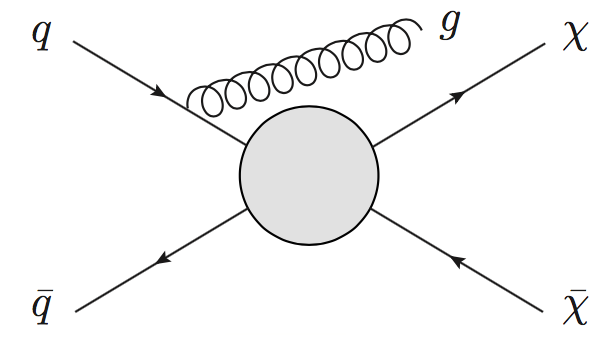
\includegraphics[width=0.9\textwidth]{Figures/1/EFT_Signature.png}
	\end{minipage}
	\begin{minipage}[b]{0.45\textwidth}
	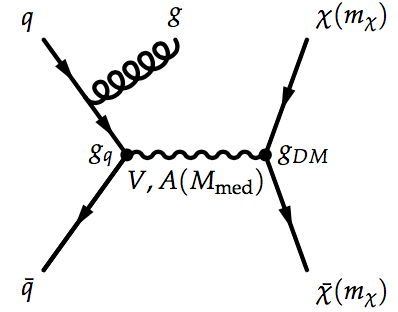
\includegraphics[width=0.8\textwidth]{Figures/1/simplified_model.png}
	\end{minipage}
	\caption[]{Left: \met+jets process in the EFT framework (figure from \(\copyright\) \cite{beyond_eft}). Right: \met+jets process in a simplified model framework, where the pair production of DM occurs via a new vector or axial-vector ($V$, $A$) mediator of mass $M_\text{med}$, which couples to quarks and DM with coupling constants g$_q$ and g$_\text{DM}$, respectively (figure from \(\copyright\) \cite{dm_forum})}.
	\label{fig:eft_simplified_model}
\end{figure}

In principle, complete theories of physics beyond the SM, such as the minimal supersymmetric SM (MSSM) (for a review, see \cite{mssm}) can offer theoretically motivated and experimentally accessible models that specify the details of candidate processes by which the colliding partons may annihilate to produce DM. However, these theories tend to be quite complex, with many free parameters - over 100 in the case of MSSM - most of which need to be fixed to generate a reasonably testable model. Relying on complete theories alone to guide experimental signatures may run the risk of missing important parameter space of new physics for which a complete theory has not yet been developed. 

Simplified models, widely used in recent and ongoing DM searches at the LHC (see, for example, the 2015 report of the ATLAS/CMS Dark Matter Forum \cite{dm_forum}), are designed to bridge the gap between EFT and complete theories. They provide a ``first-order" description of theoretically motivated new physics scenarios that could be accessible at collider energies. They provide guidance for experimental searches without fully specifying the details of any additional new physics at energies above the collider scale that would be needed for a complete theory. In terms of DM production at the LHC, one or more new ``portal mediators" associated with new physics scenarios may be considered, which allow for mixing between SM particles and DM. The process by which the mixing occurs is represented with a tree-level diagram whose experimental signature would be accessible at LHC energies, such as the diagram shown in Figure \ref{fig:eft_simplified_model}, which represents a DM benchmark model featured in Ref. \cite{dm_forum}. 

Many simplified models predict the so-called \met+X final-state signature discussed above, in which the DM is produced in association with detectable SM particles (X). Depending on the details of the hypothesized DM production mechanism and the parameter ranges considered, different models can vary widely in terms of the identity and topology of the detectable final-state particles (X) predicted in \met+X final states. Therefore, a broad-based program has been undertaken at the LHC to search for DM production in a variety of \met+X final states to ensure maximal coverage of potential DM production scenarios. Results from a selection of recent DM searches in \met+X final states can be found in Refs. \cite{monojet_cms_2021, monojet_atlas_2021, mono_hf_cms_2017, mono_hf_atlas_2018, mono_Z_atlas_2021, mono_Z_cms_2021, mono_h_cms_2020, mono_h_bb_atlas_2021, mono_h_gg_atlas_2021}.
%See, for example, results from recent searches for DM production in association with jets\footnote{Jets are produced by energy deposits of hadronized quarks and gluons in the hadronic calorimeter. See Section \ref{sec:had_calo} for a detailed discussion of the production and reconstruction of jets in the ATLAS hadronic calorimeter.}, a Z boson, 

The search presented in this thesis, which targets a final state of DM produced in association with a pair of \(W\) bosons (\met+WW), is interpreted with the ``Dark Higgs" simplified model \cite{Duerr2017} discussed in Chapter \ref{chapter:dh_model}. Searches for DM at the LHC, interpreted in the context of this model, are sensitive to DM with mass in the range of \(\sim100~\GeV\).

\section{Summary of the Thesis}

Following a brief introduction to the Standard Model (SM) of particle physics, this chapter presented multiple lines of evidence from observational astronomy for the abundance of DM in the universe, and for its hypothesized composition as one or more new particles beyond the SM. This was followed by a discussion of the ongoing worldwide effort to search for evidence of particle DM using particle detectors, and how the search presented in this thesis fits into the wider effort. 

The following chapter discusses the ``Dark Higgs" model that is used to interpret the search. Chapter 3 introduces the LHC machine and the ATLAS detector used to collect the particle collision data. Chapter 4 introduces the Monte Carlo method and its application to modelling the expected yields of events in the ATLAS detector, both from the Dark Higgs signal process and from known Standard Model processes that constitute a background in the search. The reconstruction and analysis of the ATLAS collision data is discussed in Chapter 5, and Chapter 6 presents the methods used to quantify the impacts of uncertainties from theoretical and experimental sources. Chapter 7 discusses the statistical framework used to interpret the results of the search. Chapter 8 presents the range of Dark Higgs model parameters excluded by the search. Chapter 9 concludes with a discussion of the experimental strategy and results. 


%	\startchapter{The Dark Higgs Model}
\label{chapter:dh_model}


%	\startchapter{Introduction to the LHC and the ATLAS Detector}
\label{chapter:lhc_atlas}

The Large Hadron Collider (LHC) \cite{lhc_machine} is a circular proton-proton (\(pp\)) collider which resides in a 27 km tunnel near the European Organization for Nuclear Research (CERN). Superconducting magnets are used to accelerate counter-rotating bunched proton beams to near the speed of light, and direct the beams into head-on collisions at four interaction points around the ring. The collisions take place at a world-leading centre of mass energy of up to 13 TeV. Each interaction point is surrounded by a detector, which measures the energetic debris of particles produced by the high energy collisions to perform precision measurements of the SM and search for new physics.

The large 13 TeV centre of mass energy of the collisions makes it possible for the colliding proton constituents, known as ``partons", to pair annihilate and subsequently produce massive unstable particles such as the Higgs boson, which cannot presently be produced by any other experimental means. Experiments at the LHC can study hypothetical models of physics beyond the SM (``BSM physics") by searching for evidence of the production of the massive particles involved in these models from their subsequent decay to SM particles.

The LHC also collides protons at a world-leading collision rate, \(\sim\)100 times higher than the next-leading proton collision rate at the Tevatron collider \cite{tevatron} which operated from 1983-2011 and collided protons and anti-protons (\(p\bar{p}\)) at a peak centre of mass energy of 1.8 TeV. Over several years of data-taking, the high collision rate at the LHC has enabled experiments to collect rich data sets. These large data sets enable searches for new physics to study highly selective subsets of the data in which signatures of new physics are predicted.
%, while still maintaining a sufficient amount of data in these subsets to make statistically significant comparisons with SM predictions to search for excesses in the data that could arise from new physics.

\section{The Parton Model}
\label{sec:parton_model}

Before discussing \(pp\) collisions at the LHC in detail, it is important to first introduce the parton model which describes the substructure of protons involved in the collisions. 

The proton has an internal structure comprised of constituent quarks, antiquarks and gluons - collectively known as ``partons" - and their interactions \cite{parton_model}. When a proton collides with another particle in particle colliders such as the LHC, the probability density \(f(x, Q^2)\) that a particular species of parton, for example a quark with ``up" flavour \(u\), will be involved in the collision is a function of both the fraction \(x\) of the proton's momentum carried by the parton, and the squared momentum scale \(Q^2\) of the collision. Detailed parameterized models of the parton distribution function (PDF), such as MSHT20 \cite{MSHT20} have been developed using combined fits to data from deep inelastic scattering (DIS) experiments at proton colliders. MSHT20 PDF models at \(Q^2\) of 10 GeV\(^2\) and \(10^4\) GeV\(^2\) are shown in Figure \ref{fig:msht20_pdfs}.

\begin{figure}[H]
	\centering
	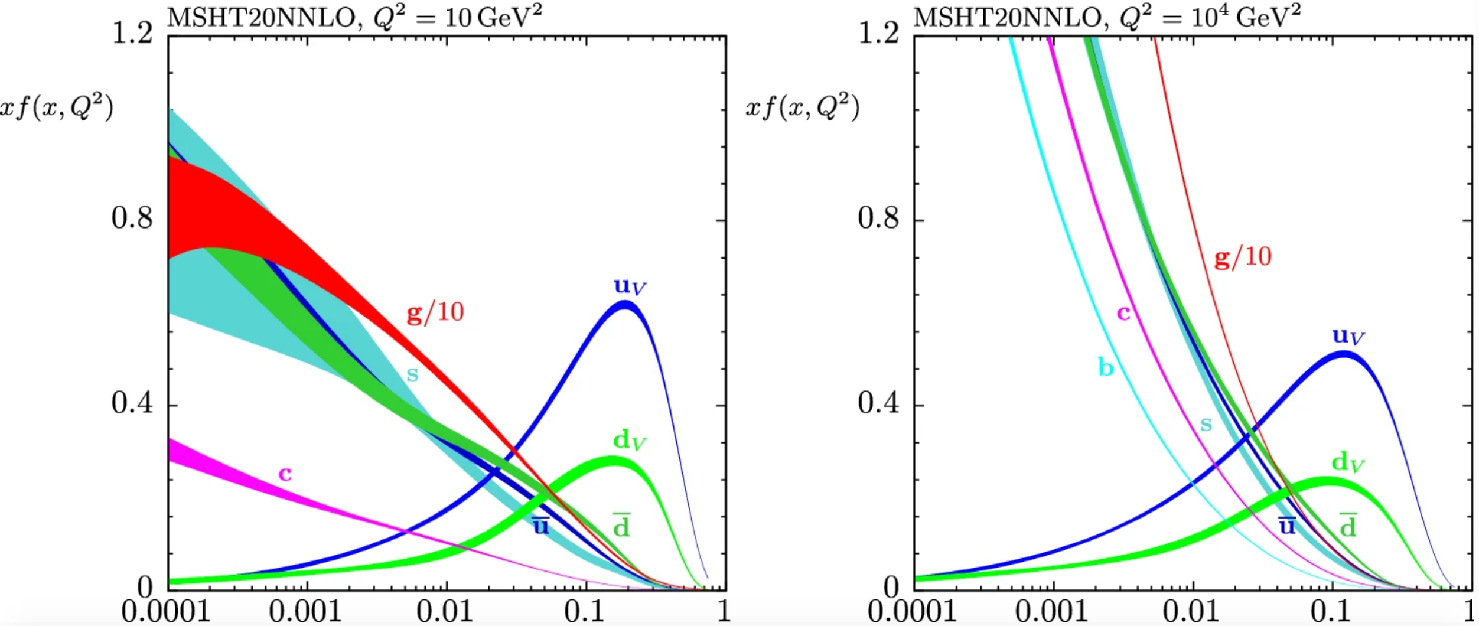
\includegraphics[width=0.9\textwidth]{Figures/3/MSHT20_PDFs.pdf}
	\caption[]{Parton distribution functions modelled with MSHT20 at \(Q^2=10\) GeV\(^2\) and \(10^4\) GeV\(^2\). Figure from \(\copyright\) \cite{MSHT20}.}
	\label{fig:msht20_pdfs}
\end{figure}

Based on the PDFs shown in Figure \ref{fig:msht20_pdfs}, \(u\) and \(d\) quarks carry the highest probability density for parton momentum fractions above \(\sim\)10\%, with the \(u\) carrying approximately double the probability density of the \(d\). These dominant quarks are known as the proton's ``valence" quarks, of which there are two \(u\) and one \(d\), and they carry the proton's quantum numbers.

\section{Decay Processes from Parton Collisions}
\label{sec:decay_processes}

Each process of particle production initiated by high-energy particle collisions at the LHC proceeds with a certain probability relative to other processes that could also be initiated by the same collision. The probability that a given process will take place is quantified by its ``cross section" \(\sigma\). The beam luminosity \(\mathcal{L}\) relates the rate of collisions \(\frac{dN}{dt}\) which proceed via a given process to the cross section of the process:

\begin{equation}
\frac{dN}{dt} = \mathcal{L}\sigma
\end{equation}

The luminosity can be integrated over a period of time \(t_1\) to \(t_2\), such that the total number of events expected to be produced via a process with cross section \(\sigma\) over the given period is related to the ``integrated luminosity" \(\mathcal{L}_\text{int}\) by:

\begin{equation}
N = \sigma\int_{t_1}^{t_2}\mathcal{L}(t)dt = \sigma\mathcal{L}_\text{int}
\end{equation}

Figure \ref{fig:ATLAS_xsections} shows a summary of cross sections for the production of SM particles - or particle combinations (eg. ``\(Wt\)" represents the production of a W boson along with a top quark) - from \(pp\) collisions at the LHC, as measured by the ATLAS detector \cite{atlas}. 

\begin{figure}[H]
	\centering
	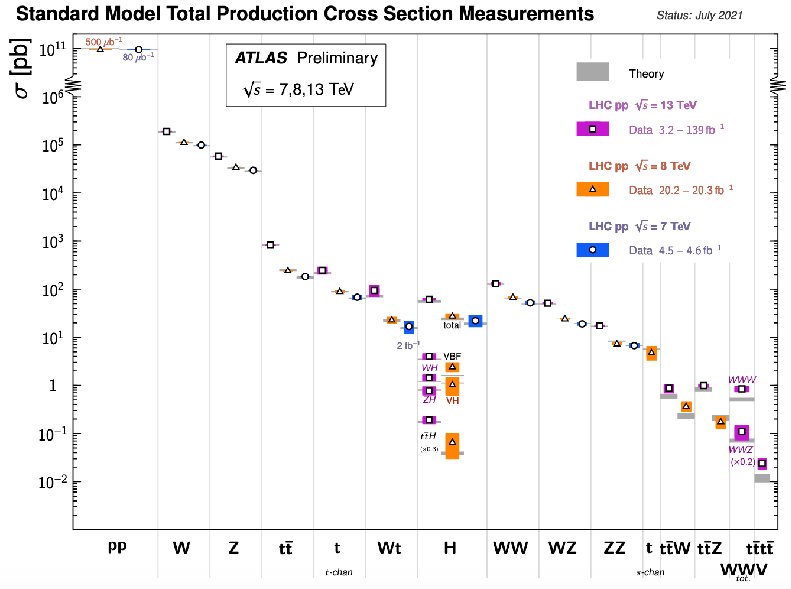
\includegraphics[width=0.9\textwidth]{Figures/3/ATLAS_xsections.pdf}
	\caption[]{Summary of SM cross sections for particle production processes measured by the ATLAS detector. Figure from \(\copyright\) \cite{ATL-PHYS-PUB-2021-032}.}
	\label{fig:ATLAS_xsections}
\end{figure}

\subsection{Branching Fractions and \(W\) Boson Decays}

Unstable particles produced by the parton collisions will subsequently decay to less-massive particles, typically with multiple possible mechanisms, also known as ``channels", by which the decay can occur. Each such channel has an associated ``branching fraction", which quantifies the relative probability with which the decay will proceed by the given channel. The search presented in this thesis focuses on DM production in association with a pair of oppositely-charged W bosons. Figure \ref{fig:W_decays} shows the two \(W\) boson decay routes. Due to energy and momentum conservation, W bosons can only decay to a pair of particles whose combined mass is smaller than the W mass. Charge conservation additionally requires that the decay products have a combined charge equal to that of the parent W boson. These two requirements allow the W to decay either ``hadronically" to a quark-antiquark pair with one up-type quark/antiquark (U) and one down-type (D), or ``leptonically" to a charged lepton (L) and a neutrino (\(\nu\)).

\begin{figure}[H]
	\centering
	\begin{subfigure}[b]{0.49\textwidth}
	\centering
	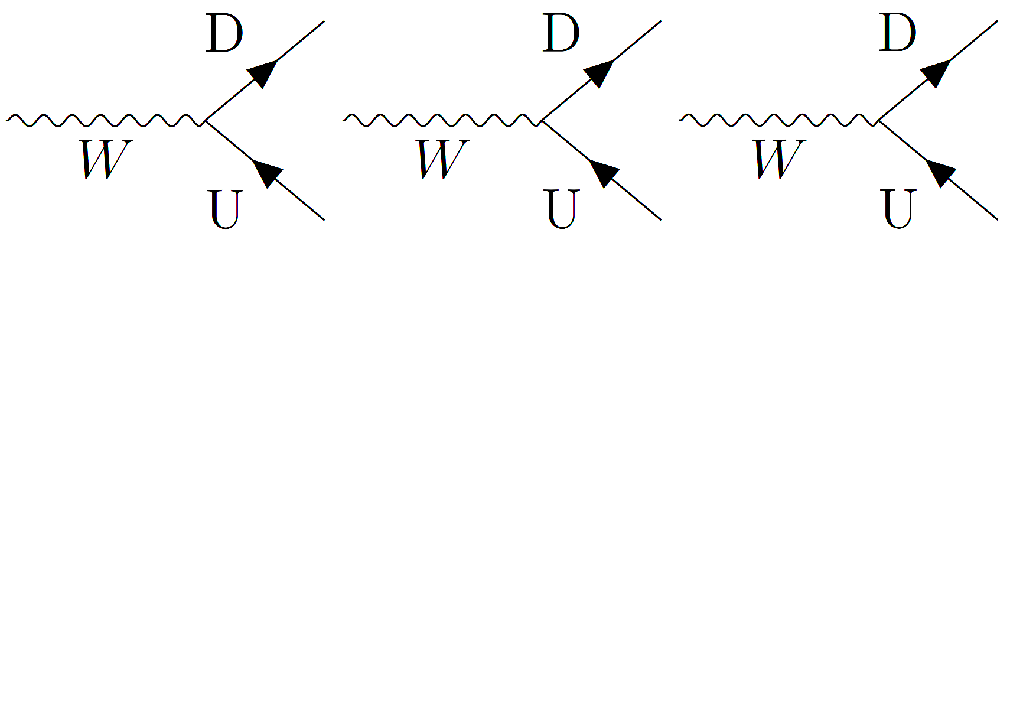
\includegraphics[width=0.45\textwidth]{Figures/3/W_had_decay.pdf}
%		\begin{tikzpicture}
%			\begin{feynman}
%		 		\vertex (a);
%				\vertex at ($(a)+(1.5cm, 0)$) (b);
%				\vertex at ($(b) + (0.9cm, 0.75cm)$) (c);
%				\vertex at ($(b) + (0.9cm, -0.75cm)$) (d);
%		 		
%		 		\diagram* {
%				(a) -- [boson, edge label'=\(W\)] (b),
%				(b) -- [fermion, edge label=D] (c),
%				(d) -- [fermion, edge label=U] (b),
%		 		};
%		 	\end{feynman}
%		 \end{tikzpicture}
	\caption{Hadronic decay mode}
	\label{fig:W_decays_had}
	\end{subfigure}
	\begin{subfigure}[b]{0.49\textwidth}
	\centering
	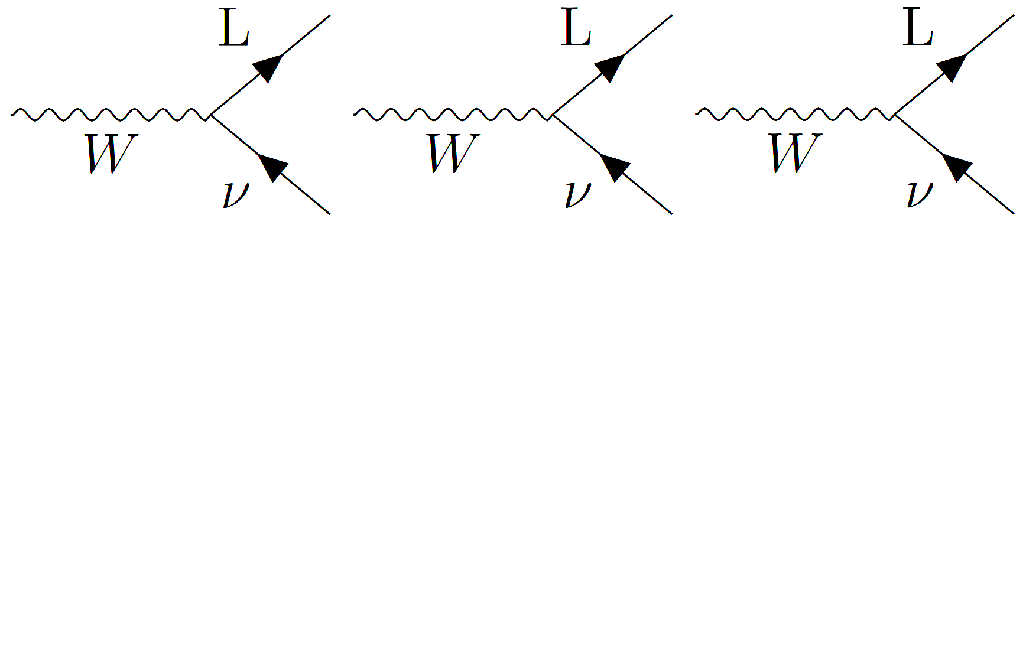
\includegraphics[width=0.45\textwidth]{Figures/3/W_lep_decay.pdf}
%		\begin{tikzpicture}
%			\begin{feynman}
%		 		\vertex (a);
%				\vertex at ($(a)+(1.5cm, 0)$) (b);
%				\vertex at ($(b) + (0.9cm, 0.75cm)$) (c);
%				\vertex at ($(b) + (0.9cm, -0.75cm)$) (d);
%		 		
%		 		\diagram* {
%				(a) -- [boson, edge label'=\(W\)] (b),
%				(b) -- [fermion, edge label=L] (c),
%				(d) -- [fermion, edge label=\(\nu\)] (b),
%		 		};
%		 	\end{feynman}
%		 \end{tikzpicture}
	\caption{Leptonic decay mode}
	\label{fig:W_decays_lep}
	\end{subfigure}
	\caption[]{W boson decay mechanisms}
	\label{fig:W_decays}
\end{figure}

\section{Detectors at the LHC}

The DM search presented in this thesis uses data collected from the ATLAS (A Toroidal LHC ApparatuS) detector \cite{atlas}. ATLAS is one of four particle detectors at the LHC which are designed to measure the energetic debris of particles produced by high energy particle collisions to perform precision measurements of the SM and search for new physics using the resulting particle collision data. This section briefly introduces each of the four particle detectors at the LHC, and what each contributes to the LHC physics programme.

The two largest, \textbf{ATLAS} (A Toroidal LHC ApparatuS) \cite{atlas} and \textbf{CMS} (Compact Muon Solenoid) \cite{cms}, are both general-purpose detectors designed to record all SM decay products from the collisions, with the exception of neutrinos which pass through due to their very low interaction cross sections. Thanks to their near-complete detection of decay products, data from these detectors can be used to study a wide range of physics processes resulting from the collisions, including both measurements of the SM and searches for new physics beyond the SM. By taking a general-purpose approach, rather than specializing in the study of one particular collision or decay process, these experiments seek to maintain sensitivity to the broadest possible range of particle processes, in the hopes of allowing physicists to detect and measure new physics processes in whatever form they may take. While the physics goals of these two detectors are very similar, they are accomplished using different detector designs and technologies, and as such they are able to produce complementary physics results.

The Large Hadron Collider beauty (LHCb) detector \cite{LHCb} is designed to measure heavy quark (\(b\) and \(c\)) decays resulting from \(pp\) collisions. Precise measurement of heavy quark decays are of particular interest for the study of CP violation in the SM, and in the search for potential sources of CP violation beyond the SM. Rather than providing full coverage of all collision products, the LHCb detector is comprised of a series of sub-detectors which provide ``forward angle" coverage to detect particles produced with a large boost along the direction of one of the two proton beams. This forward region is of particular interest for measurements of heavy quark decays, because this is the angular region in which heavy quark pairs are predominantly produced by high-energy collisions.

A Large Ion Collider Experiment (ALICE) \cite{ALICE} is designed to measure the products of heavy-ion collisions produced during special LHC runs in which the proton beams are replaced by Pb beams, which are collided at a centre of mass energy of 5 TeV. The high-energy Pb collisions produce a sufficiently high temperature and density to form an unbound state of quarks and gluons known as ``quark-gluon plasma" which would have occurred in the early universe. The study of this exotic state could give novel insights into the theory of quantum chromodynamics which describes interactions that proceed via the strong force, including the phenomena of quark colour confinement and chiral-symmetry restoration \cite{quark_confinement, Karsch:845568}.


\section{Introduction to the ATLAS detector}
\label{sec:ATLAS_detector_intro}

The ATLAS detector \cite{atlas}, shown schematically in figure \ref{fig:detector}, is the largest detector by volume to have been built at any particle collider, with a length of 44 m and a height of 25 m, constituting a total weight of approximately 7,000 tonnes. The tremendous amount of detector material is needed to absorb and measure the highly energetic decay products of the \(pp\) collisions with sufficient resolution to enable a detailed reconstruction of the particles involved and their kinematic properties. Such a complete and detailed reconstruction of the collisions and subsequent decay processes enable physicists to carry out the impressive range of physics goals shared by the ATLAS and CMS collaborations. These goals include precision measurements of the SM, which profit both from the enormous collision rate, and from the large centre of mass collision energy which enables on-shell production of all known SM particles. The detector is also designed to be sensitive to as wide a range of new physics signatures as possible. Particular emphasis was placed on designing the detector to be sensitive to the anticipated production modes of the Higgs boson, which was jointly discovered by the ATLAS and CMS collaborations in 2012 \cite{atlas_higgs, cms_higgs}. 

The detector provides full 4\(\pi\) coverage around the \(pp\) interaction point, with the exception of the beam pipe. It consists of several layers of sub-detectors, each of which is specialized for recording specific kinematic information and particle types.

The ATLAS detector is described spatially using the standard coordinate system of \((x,y,z)\) coordinates and (\(\theta\), \(\phi\)) angles shown in Figure \ref{fig:coord_system}. The origin of the coordinate system is placed at the nominal interaction point of the colliding proton beams, and the z axis lies along the beam line. The angle of a particle or detector component in the plane transverse to the beam line is given by the angle \(\phi\), and its angle relative to the beam line is given by \(\theta\). The ``pseudorapidity" \(\eta\) is a quantity related \(\theta\) according to:

\begin{equation}
\label{eq:pseudorapidity}
\eta=-\ln\Big[\tan\Big(\frac{\theta}{2}\Big)\Big]
\end{equation}

Pseudorapidity is often used rather than \(\theta\) because differences \(\Delta\eta\) in pseudorapidity are invariant under Lorentz boosts along the z axis.

\begin{figure}[H]
	\centering
	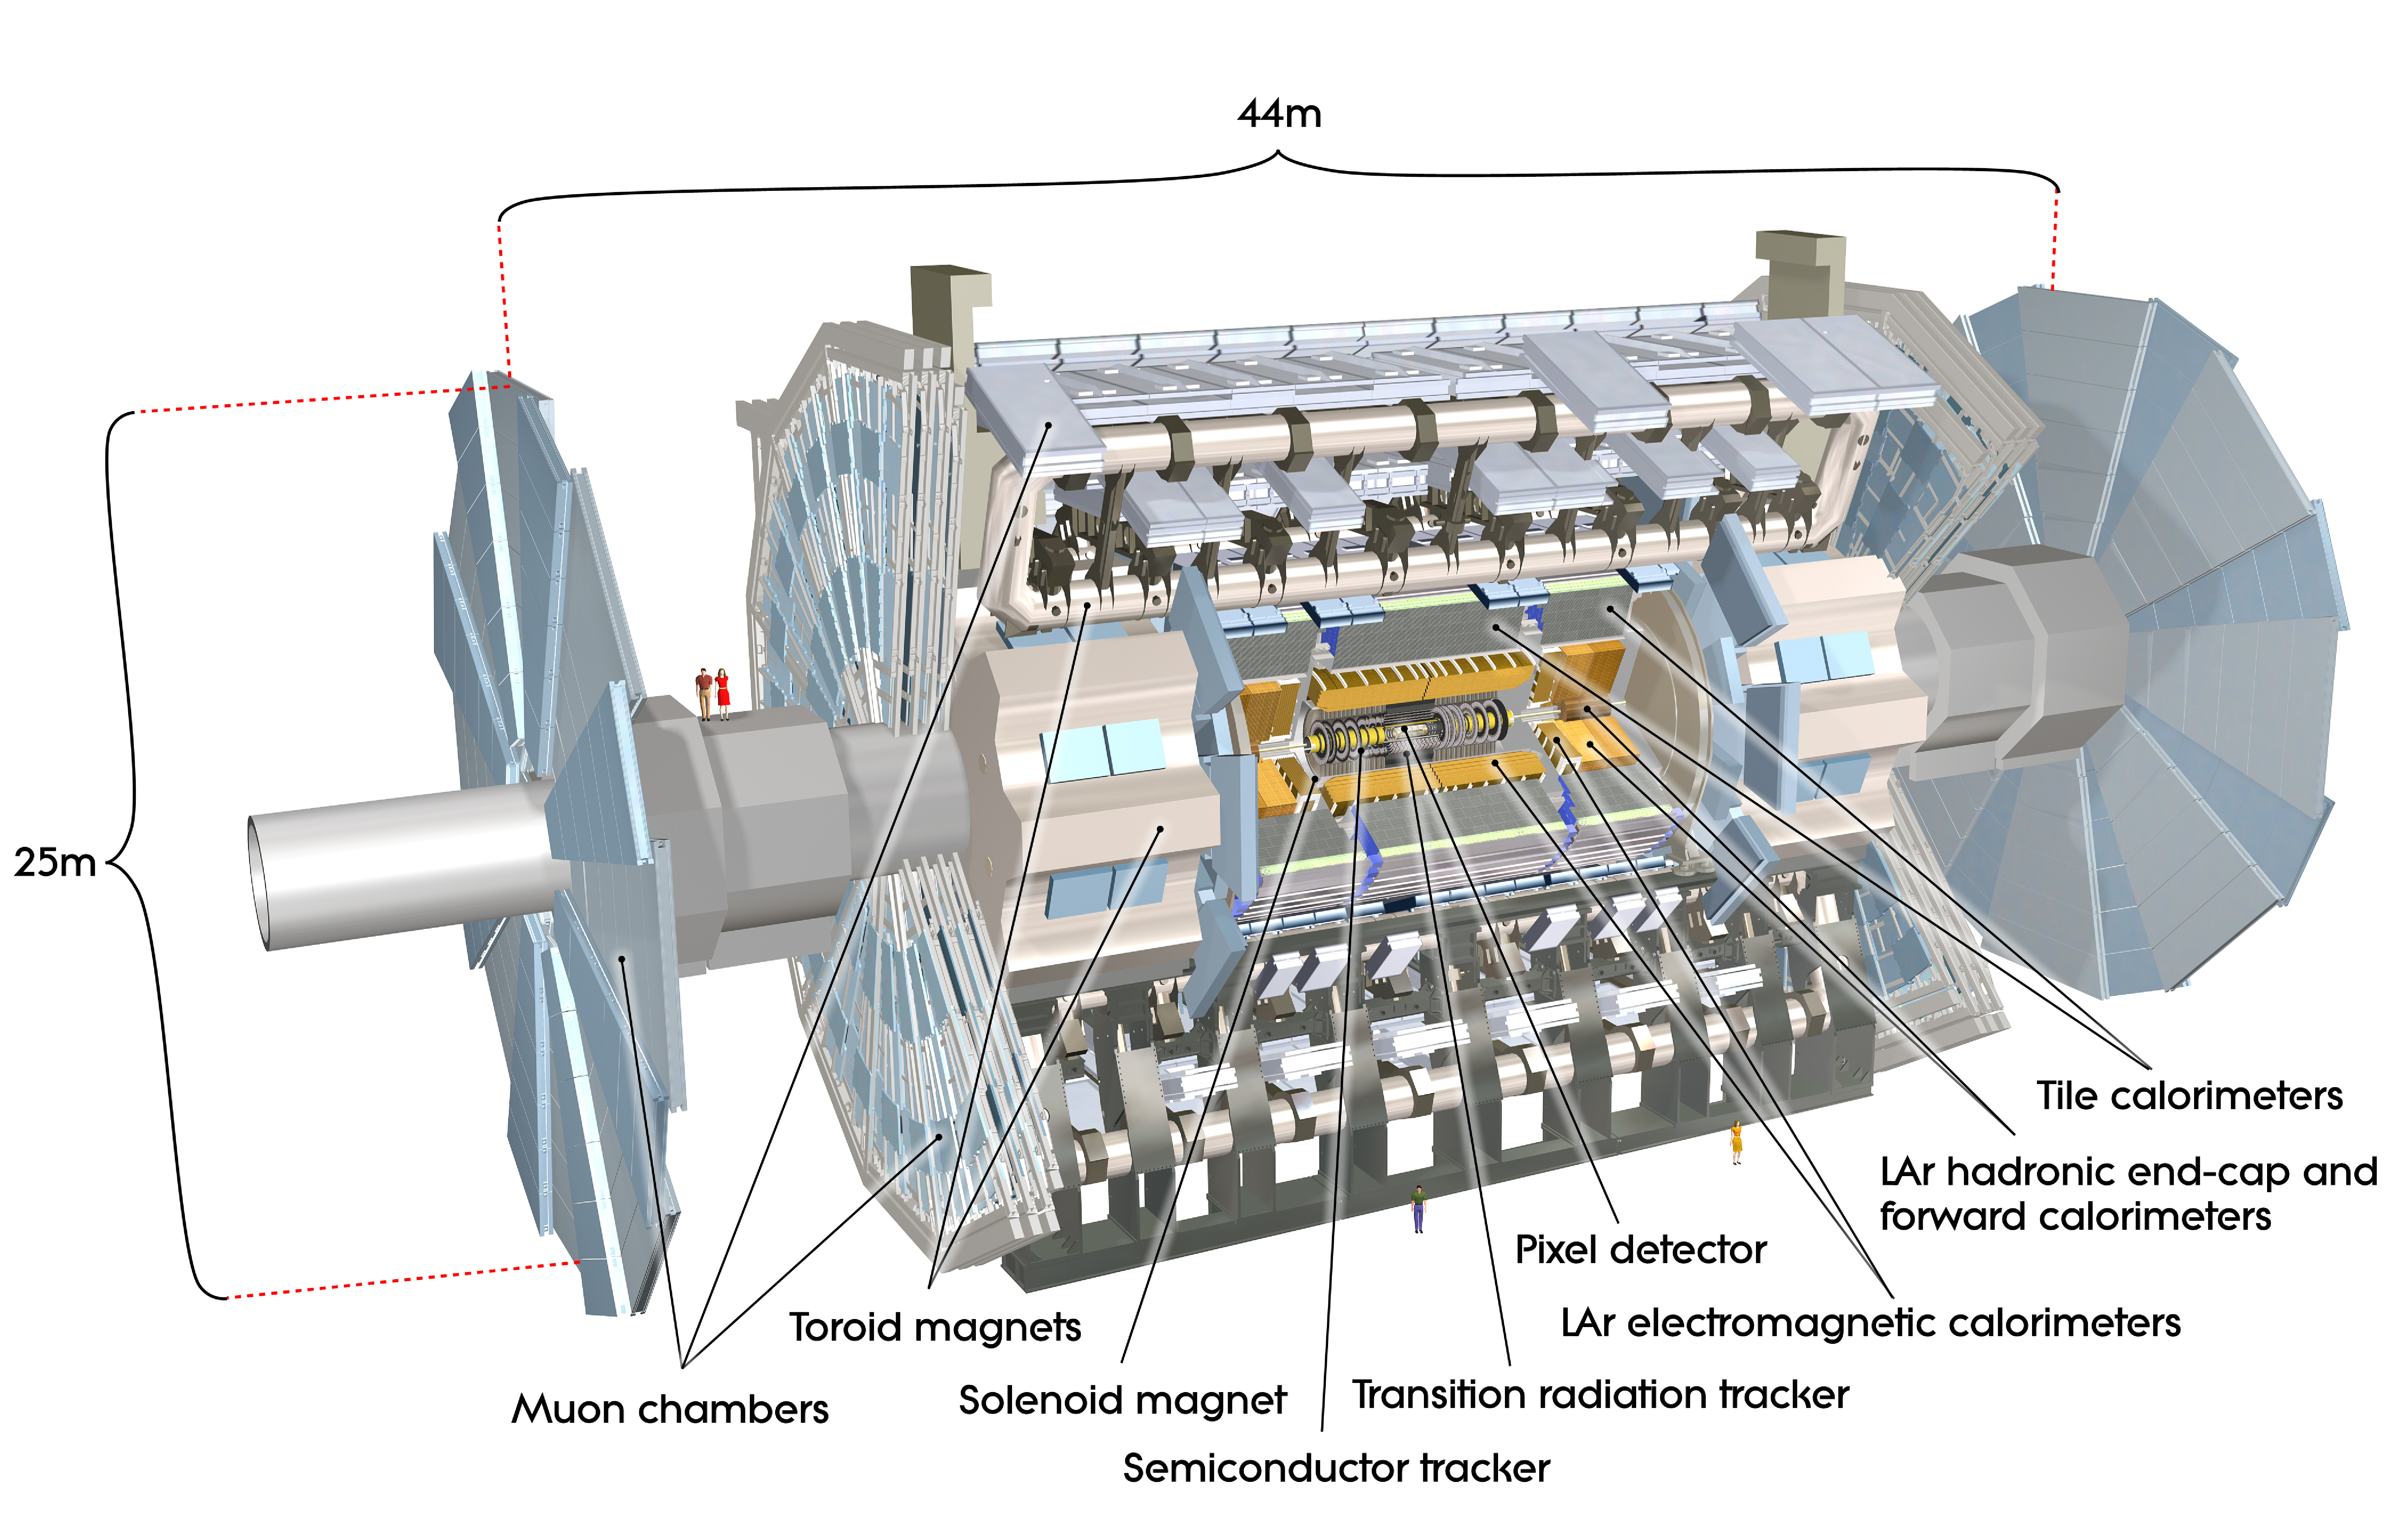
\includegraphics[width=0.85\textwidth]{Figures/3/detector.pdf}
	\caption[]{Schematic diagram of the ATLAS detector. Figure from \(\copyright\) \cite{atlas}}
	\label{fig:detector}
\end{figure}

\begin{figure}[H]
	\centering
	\begin{subfigure}[b]{0.45\textwidth}
	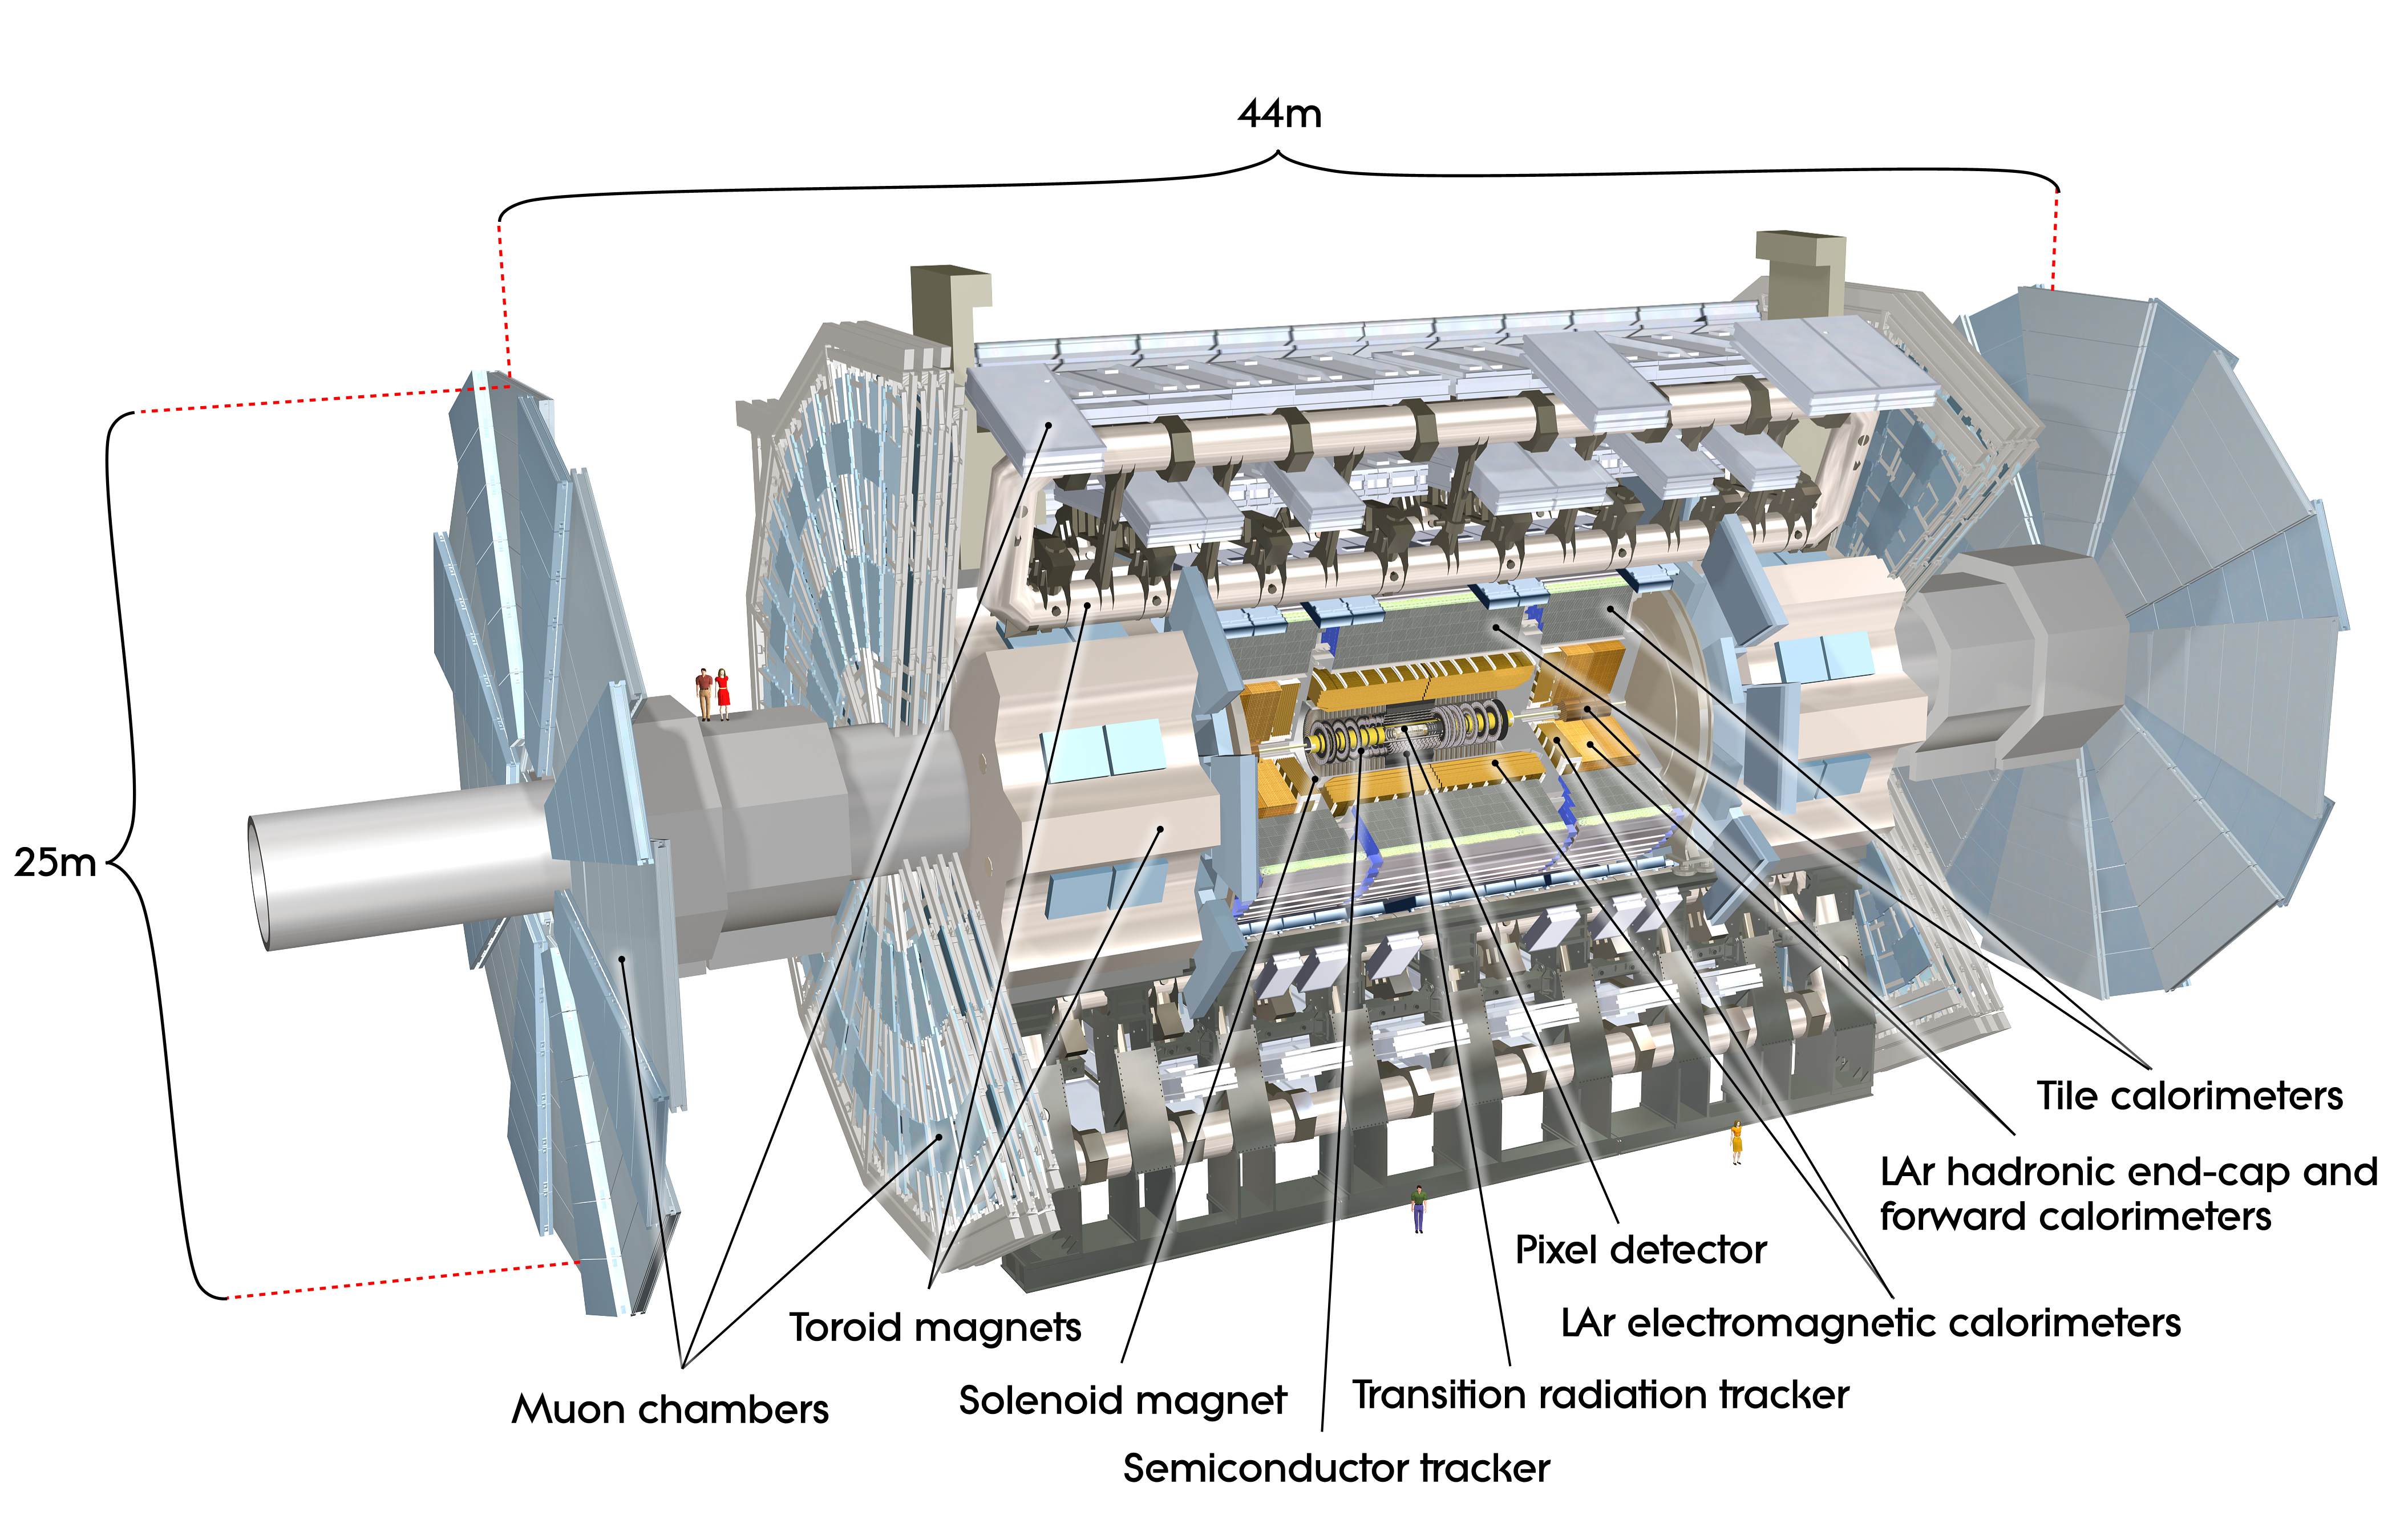
\includegraphics[width=0.9\textwidth]{Figures/3/detector.jpg}
	\caption{ATLAS Detector}
	\label{fig:detector}
	\end{subfigure}
	\begin{subfigure}[b]{0.45\textwidth}
	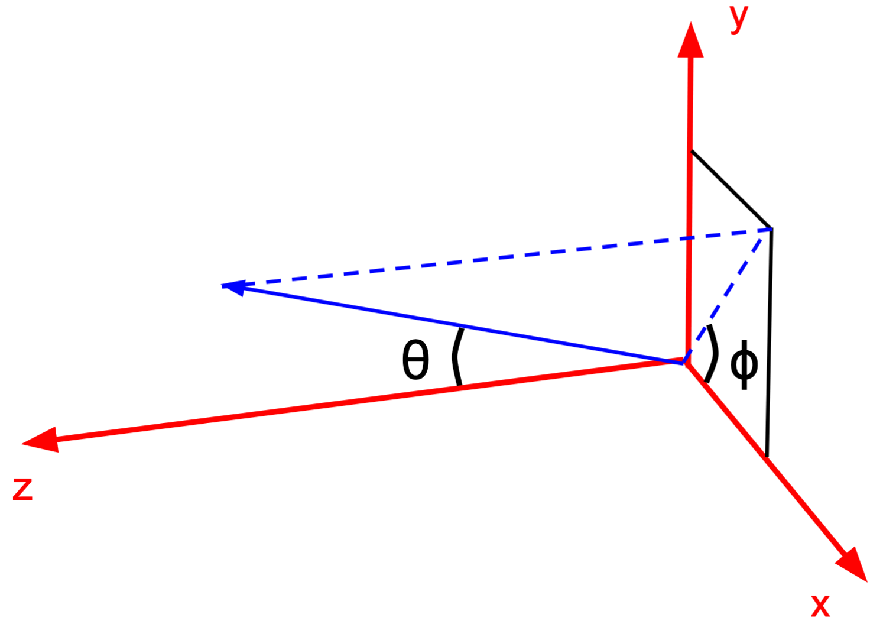
\includegraphics[width=0.8\textwidth]{Figures/3/ATLAS_coordinate_system.pdf}
	\caption{Standard coordinate system for the ATLAS Detector}
	\label{fig:coord_system}
	\end{subfigure}
	\caption[]{Left: Schematic diagram of the ATLAS detector (figure from \(\copyright\) \cite{atlas}). Right: Standard coordinate system used for the ATLAS detector.}.
	\label{fig:detector}
\end{figure}

The ATLAS sub-detectors are described in some detail in the following sections.

\subsection{The Inner Detector}
\label{sec:inner_detector}

The inner detector (ID), located nearest the beam pipe, is specialized for charged particle tracking. It is immersed in a 2T magnetic field oriented parallel to the beam pipe, which bends the trajectories (``tracks") of electrically charged particles as they pass through the field. Three distinct but complementary high-resolution tracking technologies are employed along with pattern recognition tools to map the trajectories of charged particles passing through the ID. The tracking is accomplished with as little material as possible in the ID, such that the particle trajectories can be mapped with minimal scattering and energy loss before they reach the calorimeters \cite{id_thesis}. 

Tracks from the inner detector are reconstructed by assembling clusters of ``hits" in channels of the ID tracking layers \cite{electron_reco}. The reconstructed tracks are a critical component of vertex reconstruction, and the degree of bending and direction of the bent tracks at the production vertex provide information about the momentum, charge, and identity of the charged particles that produced them. 


\subsection{The Calorimeters}

The calorimeter is designed to measure the energy of all particles which pass through it by initiating cascades of secondary particle production in the high-density detector material known as ``showers", and fully absorbing the energy of each shower. The only particles which cannot be absorbed by the calorimeter are muons and neutrinos, which pass through without showering. The calorimeter is divided into two sub-detectors, the electromagnetic and hadronic calorimeters. Both are ``sampling calorimeters", which means they are comprised of repeated layers of dense absorbing material with ``sampling" layers in between. The sampling layers track the location of the shower and record a small fraction of its energy, to which a calibration factor is applied to infer the full shower energy. 

\subsubsection{The Electromagnetic Calorimeter}
\label{sec:EM_calo}

The electromagnetic (EM) calorimeter forms the inner calorimeter layer, and is designed to fully absorb and measure the energies of electrons, positrons and photons. Energy is primarily deposited in the lead absorbing layers in the form of EM showers \cite{em_showers}, in which the initial electron or photon interacts via bremsstrahlung \cite{shower_theory} with the absorbing material to produce a cascade of photon radiation and electron pair production. The sampling layers are filled with liquid argon (LAr), which absorbs relatively little energy compared with the lead absorbing layers due to its lower density. Ionization is produced when a charged particle passes through the LAr \cite{em_cal} layer, which drifts through an electric field generated by a high voltage placed between absorber plates and readout electrodes on either end of the LAr layer to produce a triangular current pulse \cite{LAr_calo}. 

Candidate EM showers (``clusters") are reconstructed from energy deposits in calorimeter cells using a ``seed-cluster" algorithm described in Ref. \cite{electron_reco}. The seed-cluster algorithm works by dividing the \(\eta\times\phi\) space of the EM calorimeter into a grid of \(\eta\times\phi=0.025\times0.025\) solid angle elements called ``towers". For each such element, the energy detected in all the calorimeter layers which lie within the given patch of solid angle is summed to form the energy of the tower. A sliding window algorithm of size \(3\times5\) towers is used to construct energy clusters which constitute EM clusters from localized energy deposits.

Reconstruction and selection of electron candidates \cite{electron_reco} is performed with the use of a complex matching algorithm to match candidate reconstructed tracks in the ID with EM clusters in the calorimeter based on their proximity in \(\eta\times\phi\) space. This matching is complicated by the fact that electrons may radiate photons via bremsstrahlung in the ID prior to reaching the calorimeters. The radiated photons can subsequently decay into an electron-positron pair, which themselves can generate tracks in the ID. As a result, it is possible to reconstruct multiple tracks in the ID, all originating from the same electron, and match these tracks to EM clusters in the calorimeter. In case several tracks in the ID can be matched to the same EM cluster, the track considered to be associated with the primary electron is selected by an algorithm that accounts for, among other quantities, the number of hits in the ID and the distance in \((\eta, \phi)\) between the extrapolated track position in the calorimeter and the barycentre of the EM cluster. 

Reconstructed objects selected as electron candidates are subsequently passed through a likelihood-based electron identification algorithm, described in detail in Section 6 of Ref. \cite{electron_reco}, which uses as a discriminant the ratio 

\begin{equation}
\label{eq:electron_likelihood_id_discriminant}
d_L = \frac{L_S}{L_S+L_B}
\end{equation}

\noindent where the likelihood function \(L_S(B)\) is a product of signal (background) PDFs for various quantities related to the reconstructed object such as track conditions, details of the track-cluster matching, and reconstructed EM shower widths for the EM cluster in various layers of the EM calorimeter. The signal \(S\) is ``prompt" electrons, which originate from the primary interaction, and the background \(B\) is a combination of jets that mimic prompt electron signatures, electrons from photon conversions in the detector and non-prompt electrons originating from hadron decays.

\subsubsection{The Hadronic Calorimeter}
\label{sec:had_calo}

The vast majority of collision events that occur in the ATLAS detector ultimately result in the production of quarks and gluons. Due to the phenomenon of colour confinement, quarks and gluons cannot exist in isolation, and immediately ``hadronize" to form colour-neutral combinations of quarks called ``hadrons". As these hadrons pass through the detector, they eventually undergo a showering process similar in principle to the EM showers described in Section \ref{sec:EM_calo}. In the case of these ``hadronic showers", the shower is initiated by the strong interaction of a hadron with the detector material to produce a cascade of secondary hadrons \cite{shower_theory}. Unlike the EM showers which proceed exclusively via electromagnetic interactions, hadronic showers proceed via both the strong and EM interactions, where the EM interactions are primarily induced by electromagnetic decays of neutral pions (\(\pi^0\)) \cite{shower_theory}. Because hadronic showers involve strong interactions, they are in general much more complex in terms of the variety of particles and mechanisms involved in the showering, and as a result are in general more variable and less localized compared with EM showers.

The hadronic calorimeter surrounds the EM calorimeter, and is designed to fully absorb and measure hadronic showers. The primary hadrons which initiate these hadronic showers generally pass through the EM calorimeter without showering due to their relatively long interaction length \cite{atlas}. The hadronic calorimeter is comprised of a tile calorimeter which encircles the EM calorimeter barrel, and a LAr calorimeter with copper and tungsten absorbers in the end-cap region which encloses the two ends of the barrel. The tile calorimeter uses steel as the absorber material and scintillators read out by photomultiplier tubes (PMTs) in the sampling layers. 

Hadronic showers are reconstructed as ``jets" using clusters of energy deposited in the hadronic calorimeter cells \cite{jet_reco}. The jets can be reconstructed using a variety of different reconstruction algorithms depending on the use case. 

Most jet reconstruction algorithms use clusters of topologically connected calorimeter cells known as ``topo-clusters" as basic building blocks for jet reconstruction. Topo-clusters are designed with the goal of extracting significant signals of energy deposition originating from energetic hadrons from the background of detector noise and other sources of fluctuation in the calorimeter cells. Candidate clusters are formed from ``seed cells" in which the deposited energy \(E\) is \(E>S\sigma_\text{cell}\), where \(\sigma_\text{cell}\) is the average noise for the given cell and \(S\) is the ``seed threshold" significance, set to 4 by default \cite{topo_cell_clustering}. Cluster construction proceeds by collecting neighbouring cells with energy \(E>N\sigma_\text{cell}\), where \(N\) is the ``growth threshold", set to 2 by default. If a neighbouring cell passes the \(E>N\sigma_\text{cell}\) requirement, its neighbours will also be added to the cluster if their energy significance exceeds the growth threshold, and this process repeats until there are no remaining neighbouring cells with significance above the growth threshold. Lastly, one set of neighbouring cells which satisfy \(E>P\sigma_\text{cell}\) are added to the cluster, where \(p\) is the ``principal cell filter", set to 0 by default.

Jets are reconstructed from these topo-clusters using the anti-\(k_t\) clustering algorithm described in Ref. \cite{akt_algo} in a cone with an angular radius \(R\) in \((\eta, \phi)\) space, given by:

\begin{equation}
\label{eq:jet_radius}
R = \sqrt{\eta^2 + \phi^2}
\end{equation}

The jet radius \(R\) determines the angular radius within which the anti-\(k_t\) algorithm will include calorimeter deposits in the vicinity of a topo-cluster or a set of topo-clusters and attempt to group the energy deposits into jets. Different choices of \(R\) can be used in the algorithm depending on the identity and kinematics of the shower parent particle(s) that one is interested in reconstructing \cite{jet_reco}. Jets produced by quarks and gluons which either originate from different parent particles, or whose shared parent particle has a relatively low momentum in the lab frame (a.k.a. ``low boost"), generally have sufficient angular separation that they can be individually reconstructed using relatively small radius parameters such as \(R=0.2\) or \(R=0.4\). 

Jets which originate from boosted massive particles, such as the hadronically decaying \(W\) boson in the search presented in this paper, generally contain two or more significant topo-clusters (a.k.a. ``prongs") in close angular proximity, each having been induced by the hadronization of a strongly interacting daughter particle produced by the hadronic decay of the massive parent particle. In this latter case, the angular proximity of these significant topo-clusters can make it challenging to usefully reconstruct them as individual small-radius jets due to the resulting jet overlap. In these cases, it may be more useful to capture all the decay products in a single jet reconstructed with a larger radius parameter such as \(R=0.8\) or \(R=1.0\), such that the resulting large-radius jet fully reconstructs the massive parent particle. Methods such as the TAR algorithm \cite{TAR_algo} employed in this analysis are subsequently applied to the reconstructed large-radius jet to obtain useful jet sub-structure information, including the likely number of prongs contained within the jet.

\subsection{The Muon Spectrometer}
\label{sec:muon_spec}

The muon spectrometer \cite{atlas} surrounding the calorimeter is specialized for tracking muons and measuring their momentum. It employs the same principle used in the inner detector of applying a strong magnetic field and measuring the resulting bent trajectories of the electrically charged muons passing through to infer their momenta. 

The magnetic field is generated by rectangular superconducting ``toroid magnets" arranged azimuthally in radial planes around the beam axis, which set up a toroidal field concentric to the beam axis. In the region containing the strong field established by the toroid magnets, muon tracks are recorded by three cylindrical layers of muon tracking chambers in the barrel region and three layers of chambers arranged in wheels perpendicular to the beam axis in the end-cap region. Additional layers of fast trigger chambers deliver muon track information to the ATLAS trigger system (see Section \ref{sec:trigger}) so it can be incorporated into the event readout decision. 

Precise measurements of muon track coordinates are provided by monitored drift tubes (MDTs) in the barrel region, which cover a pseudorapidity range of \(|\eta|<2.0\)), and by cathode strip chambers (CSCs) in the end-cap region (\(2.0<|\eta|<2.7\)). The CSCs are designed to withstand the relatively high flux of energetic particles which bombard the detector in the end-cap region. These MDTs and CSCs measure track coordinates with nominal resolutions of 60 \(\mu\)m and 80\(\mu\)m, respectively, in the magnetic bending plane \cite{muon_reco}. 

High precision tracking is needed both to achieve the design performance goal of reconstructing muon transverse momenta with at most 10\% resolution for 1 TeV tracks \cite{atlas}, and to distinguish prompt muons which originate from the primary interaction from the background of non-prompt muons which arise from secondary interactions in the detector. Reconstruction and identification of prompt muons is performed by combining tracking information from the muon spectrometer and the inner detector, along with energy deposition measurements from the calorimeters. Various muon reconstruction strategies are employed, which attempt to match tracks between the muon spectrometer and the inner detector, or to match inner detector tracks with calorimeter deposits \cite{muon_reco}.

\subsection{Missing Transverse Momentum}
\label{sec:met}

Many signatures of hypothesized processes involving physics beyond the SM - including the DH model considered in this thesis - involve the production of particles which would pass through the ATLAS detector without being detected due to their extremely low interaction cross section with SM particles. Similarly, neutrinos produced in weak interactions will also pass undetected for the same reason. 

The law of momentum conservation, which requires the vector sum of momenta of all measured particles produced by a collision to match that of the initial state quarks, can be used to infer the presence of undetected particles in the collision. Because the fraction of proton momentum carried by each of the initial state quarks - described by the PDFs presented in Section \ref{sec:parton_model} - is statistical in nature, the momenta in the direction of the \(pp\) beam line cannot be known precisely. However, initial state quark momenta in the plane transverse to the beam line are in general negligibly small compared with the collision energy, so it can be expected to a high degree of precision that the final state particle momenta in this transverse plane will sum to zero. This expectation implies that collision events which produce undetected particles with an appreciable momentum in the transverse plane can be expected to exhibit a signature of high missing transverse momentum in the final state. 

This two dimensional missing transverse momentum vector for a collision event is typically denoted ``\metvec", and its magnitude ``\met". The components  of \metvec lie in the transverse \((x, y)\) plane of the detector, and are given by:

\begin{equation}
\label{eq:met_components}
E_{x(y)}^\text{miss} = -\sum_i p_{x(y), i}
\end{equation}

\noindent where the sum is over all fully reconstructed electrons, muons, photons, hadronically-decaying tau leptons and jets (a.k.a. ``hard objects"), and additionally over all other detector signals which were recorded as part of the event, but were not used as part of the construction of the hard objects (a.k.a the ``soft term") \cite{met_reconstruction}.

\noindent \metvec and \met are constructed from the components \(E^\text{miss}_{x(y)}\) as follows:

\begin{equation}
\label{eq:met_vec}
\metvec = (E^\text{miss}_{x}, E^\text{miss}_{y})
\end{equation}

\begin{equation}
\label{eq:met_mag}
\met = |\metvec| = \sqrt{(E^\text{miss}_{x})^2 + (E^\text{miss}_{y})^2}
\end{equation}

\subsection{The Trigger System}
\label{sec:trigger}

An overwhelming majority of collision events in the ATLAS detector result in ``soft quantum chromodynamics" (soft QCD) interactions which proceed via the strong force and produce only quarks and gluons which have a relatively low momentum in the lab frame - and hence are referred to as ``soft" - and which do not result in the production of any high-mass (\(\mathcal{O}(\text{GeV})\)) particles. Figure \ref{fig:detector} compares the overall cross section of all interactions resulting from \(pp\) collisions with the cross sections of processes which produce various massive SM particles. The overall collision cross section is \(\sim\)6 orders of magnitude larger than the highest cross section for producing a massive particle, namely that of the \(W\) boson. The soft QCD interactions which dominate the total cross sections are in general not of interest for the ATLAS physics programme. It would be impossible to process and save all collision events produced in the ATLAS detector, as the massive flux of these soft QCD interaction events would very quickly overwhelm the bandwidth of the data acquisition system and fill up the available offline data storage capacity. 

The ATLAS trigger \cite{ATLAS_Trigger} is designed to efficiently select a tiny minority of collision events to be read out, processed and saved to offline storage (a.k.a. ``recorded") based on a set of criteria applied to preliminary event information from the sub-detector. The criteria are designed to select for signatures from the sub-detectors that are considered likely to represent processes that will be of interest to the various analyses which study the data either to measure parameters of the SM, or to search for evidence of BSM physics.

The trigger system is divided into a hardware-based ``first level trigger" (L1 trigger) and software-based ``high-level trigger" (HLT), which collectively select events at an average rate of \(\sim\)1000 Hz from the total collision rate of 40 MHz \cite{ATLAS_Trigger}. Events must be accepted by both the L1 trigger and the HLT in order to be recorded.

The L1 trigger is based on candidate objects identified within regions of interest (``RoIs") defined by their \(\eta\) and \(\phi\) ranges. Candidate objects are divided into muons, EM calorimeter clusters, jets in the hadronic calorimeter and taus. In addition, the sums of missing transverse momentum (\met) and total energy are also constructed. Hardware level trigger decisions are designed using combinations of these reconstructed objects and sums. Events which pass the L1 trigger are subsequently processed by the HLT. The L1 trigger is designed to form the ``trigger decision" of whether to reject the event or accept it for processing by the HLT within at most 2.5 \(\mu\)s per event \cite{ATLAS_Trigger}. 

Thanks to the reduction in event rate by the L1 trigger selections, the HLT is able to use software-based algorithms to produce more complex reconstructions of the candidate objects and sums compared with the L1 trigger, and can apply more sophisticated selections on these objects. The HLT trigger decision is typically formed within 300 ms per event \cite{ATLAS_Trigger}. Objects reconstructed and considered in the HLT trigger decision include muons measured by the muon spectrometer, electrons, photons, jets, \met and tau leptons. 

The L1 trigger and the HLT each have their own ``trigger menu", which represents the compilation of all sets of selection criteria, or ``triggers" which are considered for each event. Any event which satisfies the criteria of any of the triggers in the trigger menu is kept. Both the L1 trigger and the HLT trigger menus include both triggers applied to individual objects, such as the ``\met trigger" or the ``photon trigger", as well as triggers applied to combinations of different objects.

Importantly for the analysis presented in this thesis, the \met that is reconstructed for each event by the L1 trigger and the HLT is based on calorimeter measurements, which register very little energy deposition from muons, and does not incorporate the momenta of muons detected by the muon spectrometer. As a result, in cases where the majority of \met in the event is recoiling against one or more energetic muons, the \met reconstructed for the triggers will underestimate the actual \met in the event due to the absence of muon momentum information. Because this analysis includes many events with an energetic muon in the final state, it was found that requiring events to have passed the \met trigger as part of the analysis selections removes some events with energetic muons in the final state which would have passed the other event selections. These analysis selections include a stringent lower bound on the offline-reconstructed \met which accounts for muon momenta. The solution, presented in more detail in Section zzz (\textcolor{red}{Note to Bob: plan to present the specific triggers used in this analysis in more detail in Chapter 5 ``Object Definitions, Trigger and Event Selection"}), was to additionally allow for events which pass the ``single muon" trigger.



%	\startchapter{Modelling of Signal and Background Processes}
\label{chapter:mc}

To search for evidence of new physics in the ATLAS data, it is necessary to develop an accurate model of the expected yield of both SM events (a.k.a. ``background") and hypothesized BSM events (a.k.a. ``signal") in the data, as well as their kinematic distributions. The yields and kinematic distributions of events in the data are then compared with those in the signal and background models to check for any ``above-background" significant excesses in the data that could point to the presence of BSM physics. If no significant excesses are observed, the search can exclude the signal model for the range of parameters for which the model predicts a significant above-background excess in the data.

\section{Introduction to the Monte Carlo Method}
\label{sec:mc_intro}

Like many collider experiments, the ATLAS collaboration uses the ``Monte Carlo" (MC) method to model the expected yield and kinematic distributions of SM and hypothesized BSM events in the data collected by the detector. The MC method is a computational algorithm which uses repeated sampling of random variables, where each set of randomly sampled variables represents a randomly generated ``event". 

To simulate the predicted behaviour of any given process using the MC method, a parametric model for the process is needed. The parametric model receives as input a set of variables associated with a single event (eg. kinematic information describing the partons involved in a high-energy parton-parton collision at the LHC, prior to the collision), and predicts the values of all variables of interest for the event after it has undergone the process being modelled (eg. the energy and momentum of the massive particle that would be produced from the parton-parton collision for a given particle production process). The MC method proceeds as follows: for each randomly generated event, the random variables associated with the event are passed into the model to produce a resulting set of output variables. For physical models, one is particularly interested in the set of ``observable" output variables, meaning those which can be measured experimentally in the modelled system. Given a set of these so-called ``MC simulated events", the associated set of values for each observable, which were generated by passing the events through the model, represents a random sampling of the underlying probability density distribution for that observable according to the model.  The method is useful for complex models with many free parameters, for which it would be unfeasible to develop analytical formulations of the distributions of observables predicted by the model.

The MC simulated events can then be binned into histograms in one or more observables. Assuming that, for each event, the sampling of random variables is performed ``independently" - i.e. in a manner such that the sampling of random variables for each event is unaffected by that of any other event - the number $N_i$ of events in each bin $i$ will vary randomly according to Poisson statistics with, on average, a standard deviation of $\sigma_{N_i}=\sqrt{N_i}$. Consequently, as the number of MC simulated events is increased by a factor of $\alpha$, the relative size $\frac{\sigma_{N_i}}{N_i}$ of fluctuations in each bin will, on average, decrease according to $\frac{1}{\sqrt{\alpha}}$. As a result, as one increases the number of MC simulated events, the shapes of histograms binned in the model's observables for the simulated events will become an increasingly precise approximation of the underlying probability distributions for these observables according to the model. 

\section{Monte Carlo Simulation of Events in the ATLAS Detector}
\label{sec:MC_ATLAS}

Signal and SM background models used to perform searches for BSM physics with the ATLAS detector are produced using sophisticated MC simulation of both the passage of the final-state particles through the ATLAS detector and of the physical production mechanisms for the particle collision, production and decay processes involved. For a given process, ``truth-level" information for each MC simulated event generated to simulate the process is first obtained from a random proton-proton collision by simulating the physical production mechanism for the process. An example of such a process would be the dominant \wjets SM background in this DM search, shown in Figure \ref{fig:Wjets_Feynman}.

The set of simulated final state particles, along with their kinematic information, are collectively known as the ``truth-level" event. Truth-level events can subsequently be passed through a highly detailed  simulation of the ATLAS detector \cite{atlas_sim} produced using the Geant4 toolkit \cite{Geant4}, which models how these events would actually be measured by the detector at this so-called ``reconstruction-level". ATLAS requires very large MC generated data sets (millions of simulated events per process) to adequately model the predicted probability distributions for kinematic observables over their full range of interest for the SM measurements and BSM searches that use the ATLAS data.

\subsection{Use of Alternative MC Generators}

ATLAS uses various MC simulation packages (also known as ``generators") to perform truth-level MC simulation of different physics processes. For many processes, particularly SM background processes, independent MC simulations have been performed using several different packages, and the yields and distributions of events predicted by the different packages can be compared to evaluate a systematic uncertainty associated with the choice of generator used to simulated the process. The specific generators used to model the physics processes considered in this search will be discussed in Sections \ref{sec:DH_model_sim} and \ref{sec:SM_bkg_sim}.

\subsection{Weighting and Normalization of MC Simulated Processes}
\label{sec:evt_weights}

Given a set of MC simulated events for a given process, it is often necessary to apply multiplicative ``weights" to the simulated events in order to correct their distributions and amplitude before comparing with the measured data. The weights are designed to modify the amount that a given event contributes to the amplitude of the bin to which it is assigned when the MC simulated events are binned into histograms. Rather than simply summing the number of simulated events which fall into a given bin, the simulated amplitude, or ``yield", of each bin is evaluated instead as the sum of event weights \(w\) for all events which fall into the bin:

\begin{equation}
\label{eq:weighted_bin_amplitude}
\text{simulated yield in bin \(k\)} = \sum_\text{event \(i\) in bin k} w_i
\end{equation}

The weights are broadly categorized into ``event-level" weights and ``scaling factors". Event-level weights may differ between one event and the next, and are designed to modify the shapes of simulated yield distributions in one or more observables to better represent their expected distributions in the measured data. These shape modifications may be motivated by a variety of factors, such as to account for data-taking conditions which were not known or incorporated at the time of simulation. Individual sources of event-level weights for processes simulated in the ATLAS detector are discussed in more detail in Section \ref{sec:evt_wts} below. 

After applying event-level weights to correct the shapes of the distributions, scaling factors are applied identically to all the events generated for a given process. The scaling factors are designed to scale the total simulated yield of events such that it matches the total number of events that are expected to have been produced by the simulated process in the actual measured data set. 

%To produce an accurate prediction of the yield and distributions of events in the actual ATLAS data set, it is necessary to apply individual event-level weights and overall normalization factors to the MC simulated events. 

\subsubsection{Weighting of MC Simulated Events of Particle Collision Processes}
\label{sec:evt_wts}

Event-level weights arising from a variety of sources are applied to events that were generated by the MC method to model particle collision and decay processes in the ATLAS detector. For a given process, the overall factor which is applied to weight each event relative to other events generated for the same process is the product of event-level weights:

\begin{multline}
\label{eq:evt_wt}
\text{event-level weight }i = \text{(generator weight)}_i \times \text{(pileup reweighting weight)}_i \times \\ \times \prod_j \text{(reconstruction weight j)}
\end{multline}

The ``generator weight" is a weight applied by some generators during the generation of truth-level events for various purposes. These purposes may include correcting for the generation of duplicate events at various stages of the calculation and correcting leading-order calculations to achieve the expected distributions that a more precise ``next-to-leading-order" calculation would be expected to produce. 

The ``pileup reweighting weight" is designed to account for the effects of ``pileup" \cite{pileup}. Due to the oscillatory electric fields used to accelerate protons in the counter-rotating LHC beams, protons in the beams do not form a continuous stream of particles, but are instead concentrated into regularly-spaced ``bunches" in the longitudinal beam direction \cite{acc_physics_text}. Superconducting magnets are used to direct proton bunches in the counter-rotating beams into head-on collisions, known as ``bunch crossings", at the centre of the ATLAS detector. Pileup constitutes the soft QCD collision events that take place in the same (or closely-surrounding) bunch crossings as the ``hard interaction" that actually triggered the event readout. The nominal procedure of simulating the ``hard interactions" which would produce the process being modelled does not account for the presence of these pileup interactions that would be measured by the detector as part of the readout for the triggered event. 

To correctly model the actual pileup conditions during data-taking, the soft QCD collision events that constitute these pileup interactions are either simulated \cite{MC_overlay_pileup} or collected from actual LHC collisions as so-called ``zero-bias data"\footnote{zero-bias data is collected using a dedicated trigger which fires one LHC turn after a high-\pt L1 trigger fires \cite{data_overlay_pileup}. This method ensures that the rate at which the zero-bias events are triggered is proportional to the instantaneous luminosity of the collisions. Since no other triggers are applied, the event readout for this zero-bias data is expected to be representative of the pileup background conditions.}. Each simulated hard interaction event is then overlaid with a variable number of the simulated pileup events, and the hard interaction and pileup events are weighted to produce the distribution of pileup events in the data. Since the MC simulated datasets were in many cases produced before or during data-taking, it is necessary to reweight the MC simulated events using the so-called pileup reweighting weight such that the distribution of pileup events accurately reflects the actual pileup distribution during the data-taking. To do so, the full ATLAS data-taking period is divided into ``luminosity blocks", and the average rate of pileup interactions is measured within each such luminosity block. MC simulated events are then associated with specific luminosity blocks. The pileup reweighting weights are evaluated for MC simulated events within each luminosity block to match the pileup rate in the simulated events to the average pileup rate measured during the associated data-taking period.

The ``reconstruction weights" collectively refer to weights assigned to apply corrections to quantities such as data-driven measurements of efficiency or resolution associated with the reconstruction of objects such as electrons, muons and jets that are produced in the simulated passage of events through the ATLAS detector.

\subsubsection{Scaling Distributions for Comparison with Data}

In addition to the event-level weights described in Section \ref{sec:evt_wts} above, scaling factors are applied to each signal and background process such that the predicted yield of events per bin in the MC simulated distributions for each process properly predicts the actual yield of events expected in the ATLAS data based on the integrated luminosity of the collected data set.

\medskip\noindent\textbf{Sum of Weights Normalization}

While the event-level weights can adjust the shapes of distributions of MC simulated events to match those expected in the data, the sum of these weights does not in general have any particular physical significance, and depends on the number of events that were simulated. Prior to scaling the sum of weights to the predicted yield in the data, it is therefore necessary to first normalize the sum of weights to unity by dividing by the sum over all event weights for the process: 

\begin{equation}
\label{eq:evt_wt_norm}
\text{event-level weight (normalized) }i = \frac{\text{event-level weight }i }{\sum_j \text{event-level weight }j }
\end{equation}

\noindent where the index j runs over all MC simulated events for the given process.

\medskip\noindent\textbf{Scaling to Expected Data Yield}

As discussed in Section \ref{sec:decay_processes}, the total predicted yield \(N\) of events for a given process of particle production and decay initiated by a proton-proton collision in the LHC is given by the total integrated luminosity:

\begin{equation}
\label{eq:predicted_yield}
N = \sigma\int_{t_1}^{t_2}\mathcal{L}(t)dt = \sigma\mathcal{L}_\text{int}
\end{equation}

\noindent where \(\int_{t_1}^{t_2}\mathcal{L}(t)dt\) is the integrated beam luminosity over the full data-taking period from \(t_1\) to \(t_2\) and \(\sigma\) is the cross section for the process, which quantifies the rate at which the proton-proton collisions will produce events via the process for a given beam luminosity \(\mathcal{L}\).
%relative to other processes that could also be initiated by the proton-proton collisions. 

Therefore, the final step in weighting the MC simulated events for comparison with data is to scale all the normalized weights in Eq. \ref{eq:evt_wt_norm} by the product of the cross section \(\sigma\) for the given process and the integrated ATLAS luminosity \(\mathcal{L}_\text{int}\) such that they sum to the total predicted yield \(N\) of events for the process:

\begin{equation}
\label{eq:evt_wt_norm_scale}
\text{event-level weight (normalized, scaled) }i = \big[\text{event-level weight (normalized) }i\big] \times \sigma \times \mathcal{L}_\text{int}
\end{equation}

\noindent The following calculation confirms that summing all event weights in Eq. \ref{eq:evt_wt_norm_scale}, and combining with \ref{eq:evt_wt_norm} and \ref{eq:predicted_yield} produces the total predicted yield \(N\) for the given process:

\begin{multline}
\label{eq:evt_wt_sum}
\sum_i\text{event-level weight (normalized, scaled) }i = \frac{\sum_i \text{event-level weight }i}{\sum_j \text{event-level weight }j}\times \sigma \times \mathcal{L}_\text{int} \\
 = \sigma\mathcal{L}_\text{int} = N
\end{multline}

\subsection{Comparing Data and MC Simulation to Search for New Physics}

With the MC simulated data properly weighted and normalized as described in Section \ref{sec:evt_wts} above, event selections are applied to both data and MC simulated events based on their final-state observables, such as the identity, momenta and directions of final-state particles measured by the detector. The selections, which are discussed in more detail in Section \ref{sec:evt_selections} \textcolor{red}{(Note to Bob: event selection section not yet written)}, are designed to define one or more regions of the data, known as ``signal regions" within which the MC simulation of the signal process predicts a relatively large yield of the hypothesized BSM process compared with the MC prediction of SM background processes. Within each signal region, the data and MC simulated events may be additionally binned in one or more final-state observables, and the resulting distributions of ATLAS data are compared with those of the total MC simulated SM background yields to check for any significant yield excesses or shape differences in ATLAS data which could be indicative of new physics.

\section{Simulation of the DH Signal Model}
\label{sec:DH_model_sim}

The DH signal model presented in Chapter \ref{chapter:dh_model} is simulated using a program called MadGraph 5 \cite{MG5}\footnote{\MGNLO[2.7.2](ATLAS, LCG)~\cite{Alwall:2014hca} is the particular version of MadGraph 5 used to generate the MC simulated signal events used in this search.}, which generates proton-proton collision events and calculates the matrix element at leading order to produce events associated with the Lagrangian for a given process. The Lagrangian for the DH signal model is encoded in MadGraph, with the coupling constants \(g_q\), \(g_\chi\), the mixing angle \(\theta\), and the DM mass \mchi fixed to the values specified in Section \ref{sec:dh_model_free_parameters}. The DH and \Zprime masses \ms and \mZp are left as floating parameters in the search. Therefore, MC simulated data sets are generated over a grid of \ms and \mZp. The grid was designed to cover masses for which the search is expected to be reasonably sensitive to the model. Figure \ref{fig:signalgrid} shows the \ms and \mZp masses for which MC simulated data sets were generated for the DH signal process. 

\begin{figure}[h]
	\centering
	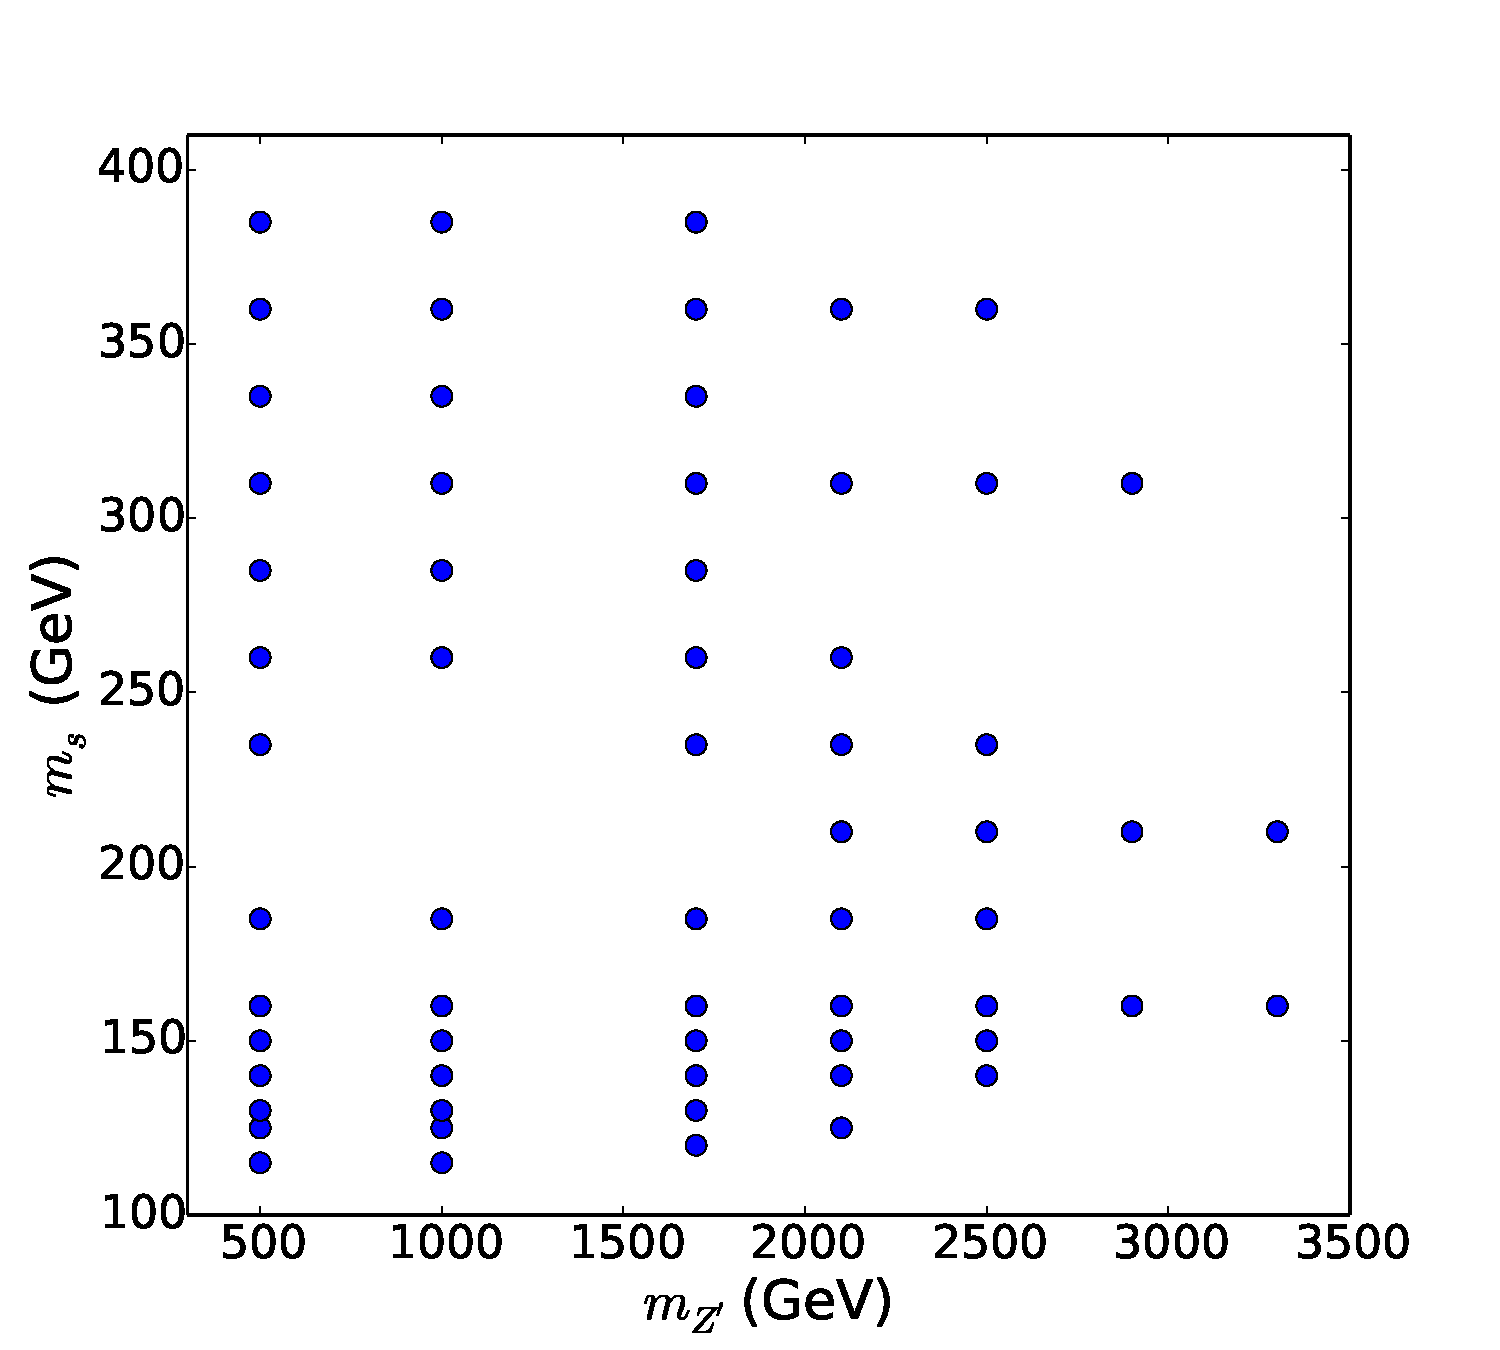
\includegraphics[width=0.8\textwidth]{Figures/4/Grid.pdf}
	\caption{Grid of produced signal samples with different choices of \mZp, \ms and the other parameters fixed to \(g_{q}=0.25\), \(g_{\chi} = 1.0\), \mchi = 200 GeV, \(\theta = 0.01\).}
	\label{fig:signalgrid}
\end{figure}

As discussed in Chapter \ref{chapter:dh_model}, the signal model considered in this search produces two final-state partons from the \(s \rightarrow WW(qq\ell\nu\)) decay. MadGraph also includes production mechanisms in the matrix element calculation for which up to one additional parton is radiated in the final state. These final-state partons initiate cascades of radiation produced by QCD processes \cite{parton_shower}, which are modelled using the Pythia8\footnote{The \PYTHIA[8.230]\cite{Sjostrand:2014zea} is the particular version of Pythia8 used to generate the MC simulated signal events used in this search.} program.

\section{Simulation of SM Background Processes}
\label{sec:SM_bkg_sim}

The selection criteria applied to final-state observables in the ATLAS and MC simulated events are designed to define signal regions which contain events that exhibit the final-state signature of the DH signal model, namely of a \(WW\) pair which decays semileptonically and which recoils against missing transverse momentum produced by the dark matter pair in the final state. However, some SM processes can produce final state observables which are similar enough to that of the signal model as to create an appreciable yield of events in the signal regions. In addition to targeting the signal model, the selections are also optimized to minimize the predicted yield of SM background processes in the signal regions. This section presents the background processes which have a non-negligible yield in the signal regions even with the optimized signal region selections.

Dominant backgrounds to the search are the \wjets, Diboson and \ttbar processes described in Section \ref{sec:dominant_bkgs}. 
%The \wjets and \ttbar processes are estimated by MC simulation in combination with the use of data-driven control region to constrain the background normalization in the combined fit. Other backgrounds are estimated purely by simulation.
Figure \ref{fig:background_yield_breakdown} shows the yield breakdowns in the signal regions of all SM background processes considered in the analysis.

\begin{figure}[h]
  \centering
     \begin{subfigure}{0.49\textwidth}
     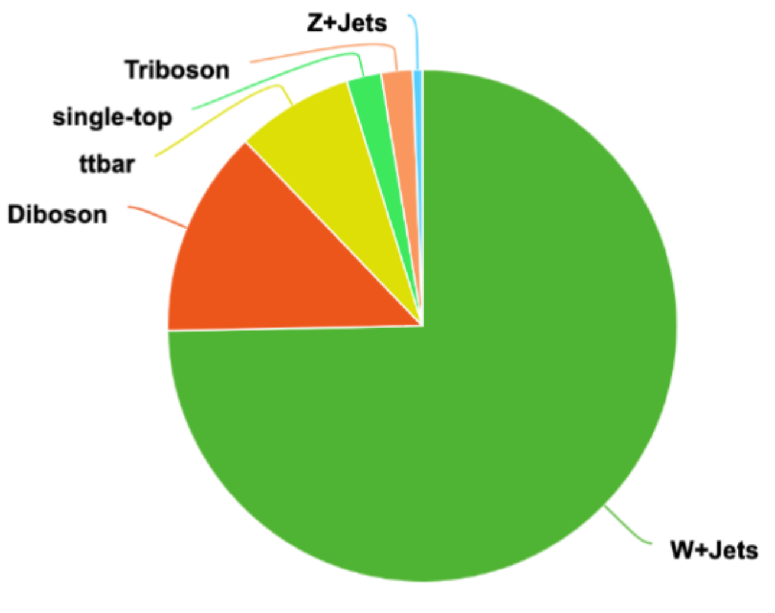
\includegraphics[width = 0.98\textwidth]{Figures/4/background_yield_breakdown_merged_SR.pdf}
    \caption{\merged SR}
    \label{fig:background_yield_breakdown_merged_SR}
     \end{subfigure}
    \begin{subfigure}{0.49\textwidth}
     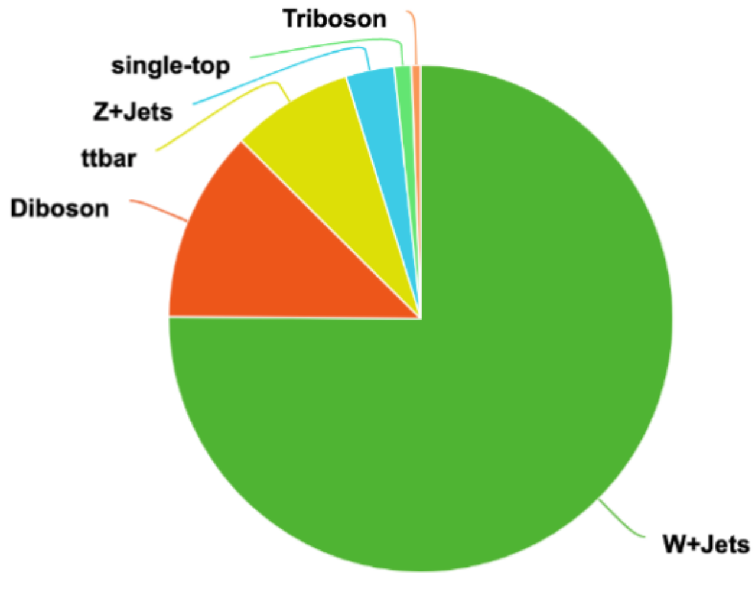
\includegraphics[width = 0.98\textwidth]{Figures/4/background_yield_breakdown_resolved_SR.pdf}
     \caption{\resolved SR}
     \label{fig:background_yield_breakdown_resolved_SR}
     \end{subfigure}
     \caption{Relative contribution of all SM background processes considered in the signal regions}
     \label{fig:background_yield_breakdown}
  \end{figure}


\subsection{Dominant Background Processes}
\label{sec:dominant_bkgs}

\subsubsection{W+jets}
\label{sec:wjets_description}

The dominant SM background in the signal regions comes from the \wjets process, wherein a leptonically decaying \(W\) is produced from the initial parton-parton collision, along with hadronic activity which fakes the hadronically decaying \(W\) in the signal model. A leading Feynman diagram for the \wjets background is shown in Figure \ref{fig:Wjets_Feynman}.

\begin{figure}[h]
  \centering
     \begin{subfigure}{0.49\textwidth}
     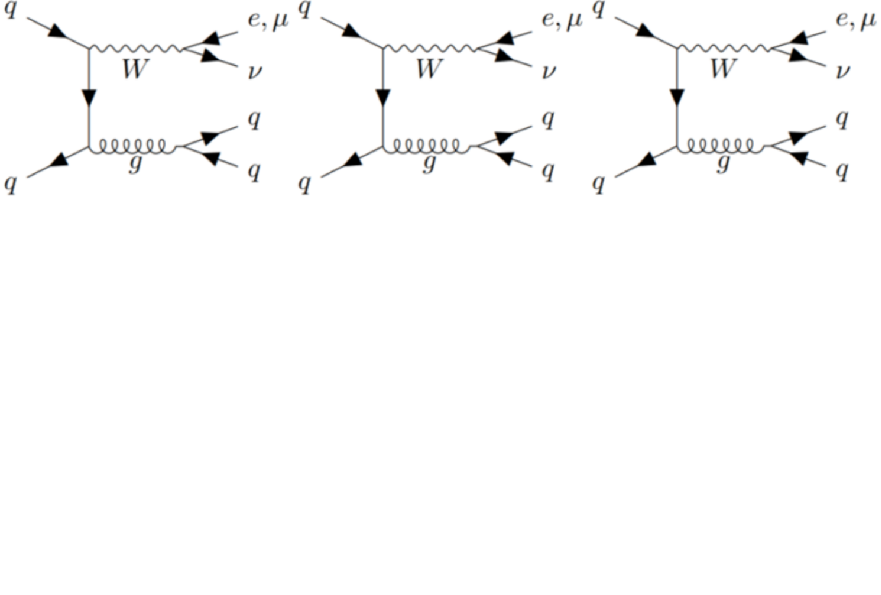
\includegraphics[width = 0.75\textwidth]{Figures/4/Fey_Wjets.pdf}
    \caption{\wjets}
    \label{fig:Wjets_Feynman}
     \end{subfigure}
    \begin{subfigure}{0.49\textwidth}
     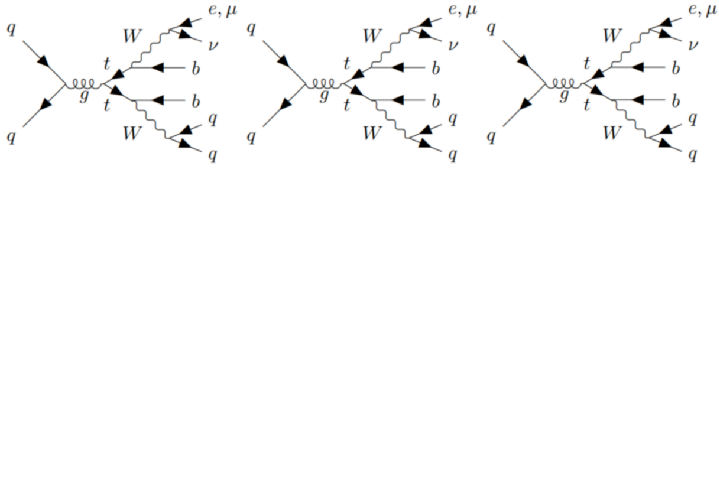
\includegraphics[width = 0.75\textwidth]{Figures/4/Fey_ttbar.pdf}
     \caption{\ttbar}
     \label{fig:ttbar_Feynman}
     \end{subfigure}
     \caption{Feynman diagrams for \wjets and \ttbar SM background processes}
     \label{fig:Feynman_bkgs}
  \end{figure}
  
The \SHERPA[2.2]~\cite{Gleisberg:2008ta} MC generator is used to model both the hard \wjets process, as well as the parton shower initiated by the final-state partons in the process. 

\medskip\noindent\textbf{Statistical Enhancement in \wjets Samples for \(m_W>120~\GeV\)}

Due to application of a high \mtlepmet requirement, described in Section \ref{sec:evt_selections} \textcolor{red}{(Note to Bob: section is not yet written)}, to reduce the \wjets background in the signal region, it was found that the majority of MC simulated events simulated for the \wjets process which make it into the signal regions are generated with a very high off-shell mass of the leptonically decaying \(W\) boson in the process \textcolor{red}{(Note to Bob/self: will need to discuss the concept of virtual and on-/off-shell production in Ch. 1)}. The default \SHERPA[2.2] generator is not optimized to produce large MC statistics in this high-\(m_W\) regime. Therefore, in addition to using samples produced by the default \SHERPA[2.2] generator, this search also makes use of a recently-developed set of specialized \SHERPA[2.2] \wjets MC generated samples\footnote{The specialized samples generated with enhanced MC statistics for large off-shell \(m_W\) are not yet discussed in any published work, but are described in the following internal ATLAS document: \href{https://cds.cern.ch/record/2753199}{ATL-COM-PHYS-2021-063}} that are generated with enhanced MC statistics for large off-shell masses (\(m_W > 120~\GeV\)) of the leptonically decaying \(W\).

\subsubsection{Diboson}
\label{sec:diboson_description}

The next-leading SM background after \wjets comes from the diboson process in which a pair of vector bosons - \(WW\), \(ZZ\) or \(WZ\) - are produced from the initial parton-parton collision. The diboson events which make it into the signal region are dominated by the production mechanism in which both bosons decay leptonically (\(W \rightarrow \ell\nu\), \(Z \rightarrow \nu\nu\) or \(Z \rightarrow \ell\ell\)) to produce a final-state lepton in addition to missing transverse momentum from the neutrino production, and one or more partons are radiated as part of the diboson production process to produce QCD activity which fakes the hadronically decaying \(W\) in the signal model. 

The diboson process, as well as the parton showers initiated by partons produced in the process, is modelled using the \SHERPA[2.2] MC generator. 

\subsubsection{\(\mathbf{t\bar{t}}\)}
\label{sec:ttbar_description}

The \ttbar process represents the third-leading SM background in the signal regions. A leading Feynman diagram for the process is shown in Figure \ref{fig:ttbar_Feynman}. In this process, two \(t\) quarks are produced from the initial parton-parton collision, both of which decay to a \(b\) quark and a \(W\) boson. The \(WW\) pair decays semileptonically, thus faking the semileptonically decaying \(WW\) pair produced in the signal model. The final-state \(\nu\) from the leptonic \(W\) decay produces the missing transverse momentum required in the signal region selection. The signal region selection includes a veto on the presence of \(b\)-tagged quarks in the final state to reduce the yield of \ttbar events, but some events from the process pass the veto and make it into the signal region due to the limited efficiency of the \(b\) quark tagging algorithm \cite{Varni:2742644}.

The production of \ttbar events is modelled using the \POWHEGBOX~v2~\cite{Frixione:2007nw,Nason:2004rx,Frixione:2007vw,Alioli:2010xd} generator which calculates matrix elements for the process. Parton showers initiated by final-state partons produced in the \ttbar process are modelled using \PYTHIA8.230~\cite{Sjostrand:2014zea}. 

\subsection{Sub-dominant Background Processes}

\subsubsection{Z+jets}
\label{sec:zjets_description}

The \zjets process is analogous to the \wjets process, but with the leptonically decaying \(W\) boson replaced by a \(Z\) boson, which also decays leptonically. For the majority of \zjets events which are classified into the signal region, the \(Z\) boson decays to a \(\ell\ell\) pair, of which one of the \(\ell\)s is not properly identified as a \(e\) or \(\mu\) during event reconstruction. 

\subsubsection{Triboson}
\label{sec:triboson_description}

The triboson process is similar in structure to the diboson, except that three vector bosons rather than two are produced from the initial parton-parton collision. Triboson events which pass the signal region selection predominantly exhibit a ``\(VVjj\)" final state in which two of the vector bosons decay leptonically to produce a final-state \(e\) or \(\mu\) in addition to missing transverse momentum from \(\nu\) production, and the third vector boson decays hadronically. The triboson process, as well as parton showers initiated by final-state partons in the process, is modelled using the \SHERPA[2.2] MC generator. 

\subsubsection{single-top}
\label{sec:stop_description}

The single-top process in the signal region is dominated by ``\(Wt\)" events \cite{stopWt} in which a single \(t\) quark is produced in association with a \(W\) boson from the initial collision of a quark and a gluon. The \(t\) quark subsequently decays to \(Wb\) to produce the signature \(WW\) final state of the signal model. As with the \ttbar background, the yield of single-top events in the signal region is reduced by the application of a \(b\)-veto in the event selection for the signal region.    

Single-top \(Wt\) associated production is modelled using the \POWHEGBOX~\cite{Re:2010bp,Nason:2004rx,Frixione:2007vw,Alioli:2010xd}~v2 generator which provides matrix elements for the process. Parton showers initiated by final-state partons produced in the single-top \(Wt\) process are modelled using \PYTHIA8.230~\cite{Sjostrand:2014zea}. 


%	\startchapter{Object Definitions, Triggers and Event Selection}
\label{chapter:objects}


%	\startchapter{Systematic Uncertainties}
\label{chapter:systematics}

In order to properly assess the significance of any discrepancies that may be seen between predicted yields and distributions of signal and SM background and the observed collision data, it is important to assign an uncertainties to all sources which may limit the precision and accuracy of the yield predictions. In addition to the limited precision of the estimates due to statistical uncertainty\footnote{See Chapter \ref{sec:mc_intro} for a discussion of the origin of statistical uncertainty in MC simulations.}, there may be inaccuracies in the values of various parameters involved in the simulation due to a limited precision with which their values are known. These inaccuracies can systematically shift predicted production rates and kinematic properties of the simulated processes, or the objects they produce in the ATLAS detector, and ultimately predicted yields and shapes of the processes in the analysis regions. Systematic uncertainties aim to quantify the maximal range of yield shifts, in each region and bin\footnote{See Section zzz \textcolor{red}{(Note to Bob: will update when section on binning is written)} for details of the binning in \minms performed in the SR})used in the search, that could result from a potential source of systematic inaccuracy. 

Systematic uncertainties (or simply ``systematics") are classified into two main categories: theoretical and experimental. Theoretical systematics account for inaccuracies that could result from a limited knowledge of parameters involved in modelling the production and decay mechanisms resulting from \(pp\) collision events at the LHC. Experimental systematics account for inaccuracies involved in the physics objects\footnote{See Section \ref{sec:object_defs} for a presentation of the reconstructed physics objects used in this search.} used to reconstruct the decay products of collision events in the ATLAS detector, and in the LHC machine itself. 

Experimental systematics are generally constrained by measurements of the ATLAS collision data in the process of calibrating the LHC machine or particular physics objects reconstructed in the ATLAS detector. Theoretical systematics, on the other hand, are often derived from a broader range of experimental 

 As a result, the confidence and precision with which theoretical uncertainties 

 obtained from experimental results from 

 some cases motivated primarily by theoretical considerations, rather than constraints from 


\begin{itemize}
\item Discussion of how systematic uncertainties are evaluated using the up/down shift in the yield within each bin obtained by varying the given source of systematic uncertainty.  
\item Clearly distinguish between theoretical and experimental sources of systematic uncertainty. Discuss the relative difficulty often involved with assigning reliable theoretical uncertainties (can be challenging to assess realistic bounds on the possible range of values for theoretical inputs, whereas experimental bounds are generally more measurable). 
\item Discussion of each major source of experimental systematics, how they're evaluated and some plots and tables showing shifts in yield arising from the dominant sources of experimental systematics.
\item Discussion of the sources of theory systematics considered (QCD scale, PDF, $\alpha_s$, PS) and how each is evaluated for signal and background.
\item Plots and tables showing the yield shifts and relative sizes of each source of theory uncertainty for signal and major backgrounds.
\item Comparison of the relative impact of statistical vs. systematic uncertainties in each analysis region, to identify where we're stats- vs. systematics-dominated.
\end{itemize}
%	\startchapter{Statistical Framework}
\label{chapter:stat}

This chapter presents the statistical framework which is used to search for evidence of new physics in the ATLAS collision data and, if no such evidence is found, establish the range of parameters over which the DH model is excluded by the search. Evidence of new physics would take the form of a statistically significant discrepancy between predicted yield distributions of SM background processes and collision data in the SRs. 

Owing to the presence of \ms-dependent peaks in the \minms distribution of the DH signal model in the SRs\footnote{See Section \ref{sec:minms} for details.}, the sensitivity of the search was found to be dramatically boosted by binning all data - MC simulated and ATLAS collision events - the SRs into several bins of \minms prior to performing the statistical analysis. Section \ref{sec:binning_strategy} presents the details of the binning strategy. Within each analysis region and bin, the statistical comparison between the observed collision data and the predicted yields of SM background and signal processes is performed by fitting the  profiled likelihood function presented in the following section to the observed collision data. The computational construction and analysis of the profiled likelihood function is performed within the HistFitter \cite{Baak_2015} statistical analysis framework.

\section{Likelihood Function}
\label{sec:likelihood}

The likelihood function which lies at the heart of the statistical framework is a product of Poisson distributions of event counts in all regions and bins:

\begin{equation}
\label{eq:likelihood_func}
\begin{aligned}
L(\boldsymbol{n}, \boldsymbol{\theta}^0|\mu_\text{sig}, \boldsymbol{s}, \boldsymbol{\mu}, \boldsymbol{b}, \boldsymbol{\theta}) & = P_\text{SR} \times P_\text{CRs} \times C_\text{syst} \\
& = \prod_{i\in\text{SR bins}} P(n_{S,i}|\lambda_{S,i}(\mu_\text{sig}, \boldsymbol{\mu_i}, s_i, \boldsymbol{b_i}, \boldsymbol{\theta})) \times \\ 
&\phantom{xxx}\prod_{j \in \text{CRs}} P(n_j|\lambda_j(\mu_\text{sig}, \boldsymbol{\mu_j}, s_j, \boldsymbol{b_j}, \boldsymbol{\theta})) \times \\
&\phantom{xxxxxlxx}C_\text{syst}(\boldsymbol{\theta}^0, \boldsymbol{\theta})
\end{aligned}
\end{equation}

where:

\begin{itemize}
    \item \(\boldsymbol{n}\in{n_{S,i}, n_j}\) is the set of all observed event counts in each region and bin.
    \item \(n_{S,i}\) and \(n_j\) are the number of observed events in the \(i^\text{th}\) bin of the SR and in the \(j^\text{th}\) CR, respectively.
    \item \(\boldsymbol{\mu}_i\) represents the normalization factors in each bin \(i\), which scale the \wjets and \ttbar backgrounds in all regions regions of the fit, with separate factors in the merged and resolved categories. The normalization factors are treated as unconstrained nuisance parameters (NPs) in the fit. They are initialized as 1 in the fit, with an uncertainty of \(\pm1\).  
    \item \(\boldsymbol{\theta}\) represents the set of NPs that parametrize all uncertainties associated with the MC simulated yields. For each normalization factor or uncertainty source \(i\), the corresponding nuisance parameter \(\theta_i\) continuously interpolates between the associated nominal and up/down shifts in predicted yield, as discussed in \Sect{4.4} of \Refn{~\cite{Baak_2015}}. For systematics sources, the NPs are normalized in the HistFitter framework such that \(\theta_i=0\) for the nominal yield, \(\theta=+1(-1)\) for the up (down) yield shift. NPs associated with statistical uncertainty of the predicted yields are instead normalized such that \(\theta=1\) represents the nominal yield in the given bin and \(\theta=1\pm1\sigma_\text{stat}/N\) represents \(\pm1\sigma\) yield shifts, where N and \(\sigma_\text{stat}\) are the expected yield in the bin and its statistical uncertainty, respectively. 
    \item The signal strength \(\mu_\text{sig}\) is an overall factor which scales the predicted yield of collision events produce by the DH signal model in all bins.
    \item \(C_\text{syst}(\boldsymbol{\theta}^0, \boldsymbol{\theta})\) is a composite function of Gaussian priors which is used to constrain the floating NPs \(\boldsymbol{\theta}\) in the fit based on their central values \(\boldsymbol{\theta^0}\) and uncertainties \(\boldsymbol{\kappa}\):

    \begin{equation}
    \label{eq:gaussian_np}
    C_\text{syst}(\boldsymbol{\theta}^0, \boldsymbol{\theta})= \prod_{j\in S} \frac{1}{\kappa\sqrt{2\pi}}e^{-\frac{1}{2}(\frac{\theta^0_j-\theta_j}{\kappa})^2}
    \end{equation}
    \noindent where \(S\) is the full set of uncertainties considered in the fit.
    
    \item The Poisson expectation functions \(\lambda_{S,i}(\mu_\text{sig}, \boldsymbol{\mu_i}, s_k, \boldsymbol{b_i}, \boldsymbol{\theta})\) and \(\lambda_j(\mu_\text{sig}, \boldsymbol{\mu_j}, s_j, \boldsymbol{b_j}, \boldsymbol{\theta})\), represent the total expected yield in each SR bin \(i\) and CR bin \(j\), respectively. 
\end{itemize}

\subsection{Poisson Expectation Formula}
\label{sec:poisson_exp}

Within a given SR bin or CR \(k\), the Poisson expectation function \(\lambda_k\) in Eq. \ref{eq:likelihood_func} is given by:
    
\begin{equation}
\label{eq:lambda}
        \lambda_k(\mu_\text{sig}, \boldsymbol{\mu_k}, s_k, \boldsymbol{b}_k, \boldsymbol{\theta}) = \mu_\text{sig}s_k\eta_{k, \text{sig}}(\boldsymbol{\theta}) + \sum\limits_{p\in{\text{\{SM bkg processes\}}}} \mu_{k,p} b_{k,p}\sigma_{k,p}(\boldsymbol{\theta})
\end{equation}
    
\noindent where \(s_k\) (\(b_{k,p}\)) is the yield of the signal process (SM background process \(p\)) predicted by MC simulation, as discussed in Section \ref{sec:MC_ATLAS}. \(\eta_{i,s}(\boldsymbol{\theta})\) is a scaling factor, nominally set to 1, which parametrizes the variations in expected yield induced by varying the NPs \(\boldsymbol{\theta}\) in the fit:

        \begin{equation}
            \label{eq:sigma}
            \eta_{k,p}(\boldsymbol{\theta}) = 1 + \sum_{s\in\text{all systematics}}I(\theta_s(k,p), \sigma_\text{down}(k,p), \sigma_\text{up}(k,p))
        \end{equation}

        where \(I(\theta_p, \sigma_\text{down}(i,s), \sigma_{up}(i,s))\) is continuous function of \(\theta_s(k,p)\) which interpolates\footnote{HistFitter employs a 6th-order polynomial to interpolate between  \(\sigma_\text{down}(i,s)\) and \(\sigma_\text{up}(k,p)\) a linear extrapolation beyond these extrema. See \Sect{4.1} of \Refn{~\cite{Cranmer:1456844}} for details.} the relative shift in predicted yield between the up and down extrema, \(\sigma_\text{up}(k,p)\) and \(\sigma_\text{down}(k,p)\), associated with varying the given uncertainty source by \(\pm1\sigma\). 

\subsection{Nuisance Parameter Nomenclature and Correlations}

Many of the NPs which appear in the likelihood function are correlated between bins, categories, and/or processes. For example, if a given NP is correlated between all bins in the fit, the value of the NP will be the same within all bins: \(\theta_s(k, p) \rightarrow \theta_s(p)\). The names given to NPs in the HistFitter framework reflect the presence of any such correlations by omitting the correlated parameter in the NP name. Taking the above example of an NP which is correlated between all bins, this correlation will be reflected by the omission of any bin number specification (eg \verb|_bin1|) 

The background normalization factors \(\boldsymbol{\mu}\) and uncertainty-related NPs \(\boldsymbol{\theta}\) are broken down as follows:

\begin{equation}
\label{eq:norm_factor_breakdown}
\boldsymbol{\mu}\in\{\mu_\text{\wjets, merged}, \mu_\text{\wjets, resolved}, \mu_\text{\ttbar, merged}, \mu_\text{\ttbar, resolved}\}
\end{equation}

\noindent and

\begin{equation}
\label{eq:norm_factor_breakdown}
\boldsymbol{\theta}\in\{\boldsymbol{\theta}_\text{statistical}, \boldsymbol{\theta}_\text{sys, exp}, \boldsymbol{\theta}_\text{sys, theory}\}
\end{equation}

Table \ref{zzz} summarizes the correlations present for each type of NP, and the scheme used in HistFitter to assign names to each.

\begin{table}
\centering
\caption{Summary of correlations between nuisance parameters in the likelihood function}
\label{tab:theo_sys_summary}
%\begin{tabular}{l p{6cm} l l }
\footnotesize{
\begin{tabular}{l p{4cm} p{4cm} l }
\toprule
\textbf{NP Type} & \textbf{Description} & \textbf{Correlation Info} & \textbf{Naming Scheme} \\
\midrule
\midrule
\(\mu_\text{\wjets, mgd}\) & Normalization factor which constraints the \wjets background in all bins of the merged category & Correlated between all analysis regions and bins in the merged category. & \(\mu_\text{\wjets, mgd}\) \\
\midrule
\(\mu_\text{\wjets, mgd}\) & Normalization factor which constraints the \wjets background in all bins of the merged category & Correlated between all analysis regions and bins in the merged category. & \(\mu_\text{\wjets, mgd}\) \\
\midrule
\bottomrule
\end{tabular}}
\end{table}


\section{Binning Strategy}
\label{sec:binning_strategy}


\begin{itemize}
\item Present the methods used in HistFitter to handle different types of uncertainty in the fit
\begin{itemize}
\item Global normalization uncertainties
\item Correlated uncertainties of shape and normalization
\item Statistical uncertainty in each bin associated with MC simulation
\end{itemize}
\end{itemize}
\begin{itemize}
\item Presentation of how normalization factors for the \wjets and \ttbar backgrounds are constrained in the CRs using a background-only fit and extrapolated to the SRs. 
\item Discussion of the evaluation of transfer factor systematics for the \wjets and \ttbar backgrounds to account for the above normalization constraint and extrapolation procedure.
\item Presentation of the discovery test to be done after unblinding $\rightarrow$ check if any fits for signal strength with unblinded data produce a statistically significant inconsistency with 0.
\item Presentation of the profiled log-likelihood ratio $q_{\mu_\text{sig}}$, and description of how $q_{\mu_\text{sig}}$ is used to calculate a p-value for the exclusion hypothesis test (in case no significant excess found in the discovery test).
\item Discussion of the use of the asymptotic formula to avoid the need to throw random pseudo-experiments when evaluating the p-value, and its regime of validity ($>\mathcal{O}(5)$ events per bin).
\item Brief discussion of the CLs method for limit setting.
\item Description of how the limits are presented in the \ms vs. $m_{Z'}$ plane.
\end{itemize}

%	\startfirstchapter{Results}
\label{chapter:results}

This chapter presents the results of applying the statistical analysis presented in Chapter \ref{chapter:stat} to the MC simulated and observed yields of ATLAS collision events in all analysis regions and bins\footnote{See Section \ref{sec:evt_selections} for details of the selections applied to define the regions used for the search, and Section \ref{sec:binning_strategy} for details of the strategy used to bin data in the SRs.} to search for evidence of new physics in the SRs. No significant discrepancy is found between the predicted yields of SM background processes and the collision data in the SRs, so the exclusion hypothesis test described in Section \ref{sec:hypo_test} is used to determine the parameter space of the DH model that is excluded by the search.


\section{Background-only Fit}

This section presents the results of performing the ``background-only" fit of the predicted yields of SM background processes obtained from MC simulation to the observed yields of ATLAS collision events in the CRs, as described in Section \ref{sec:extrapolation}, with the goal of obtaining data-driven constraints for the normalizations of the \wjets and \ttbar backgrounds within each kinematic category.

\subsection{Pre- and Post-Fit Yields of MC Simulated Background Events}

Figure \ref{fig:before_after_CRs} compares the total predicted yield of all SM background processes considered in the CRs with the yield of observed events in the ATLAS collision data, both before and after the background-only fit in the CRs. The observed yield of ATLAS collision events is consistent with the pre-fit predicted yield of SM background events within the combined statistical and systematic uncertainties in all CRs, with the exception of the merged CRTT. In the merged CRTT, a slight overprediction of the SM background yield is observed. 

The uncertainty of the total expected yield of SM background processes is reduced in all CRs after the fit, as the post-fit uncertainty is predominantly set by the Poisson uncertainty associated with the observed event counts.

\begin{figure}[h]
  \centering
  \begin{subfigure}{0.45\textwidth}
    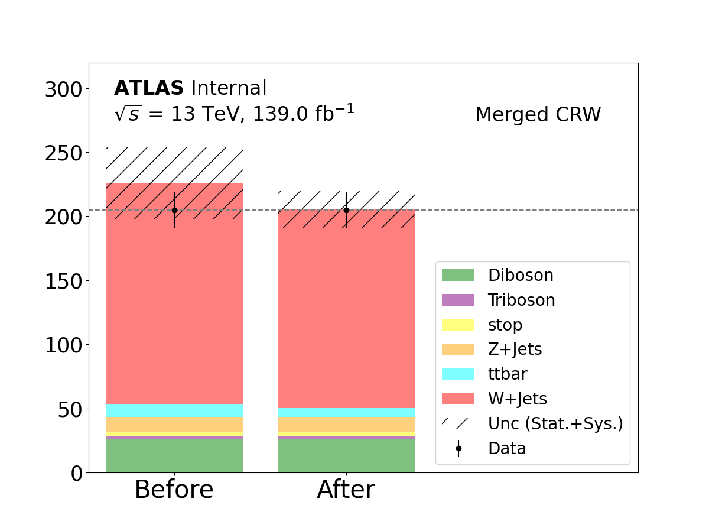
\includegraphics[width=\textwidth]{Figures/8/CRW_Merged_before_after.pdf}
    \caption{Merged CRW}\label{fig:before_after_CRW_merged}
  \end{subfigure} \hspace{1em}
  \begin{subfigure}{0.45\textwidth}
    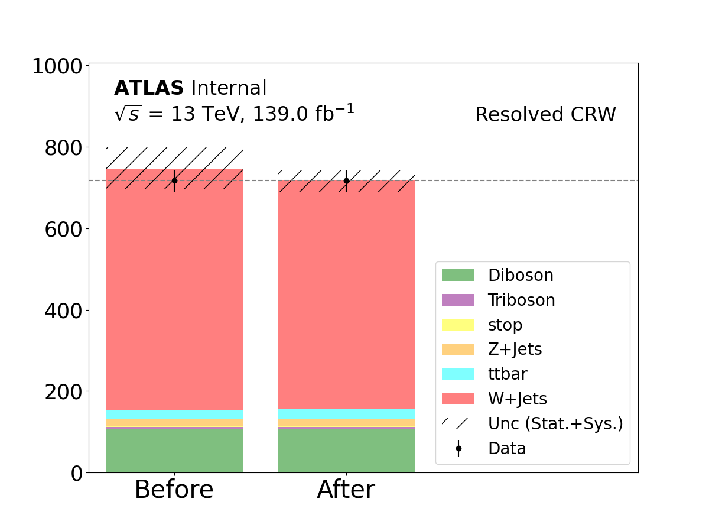
\includegraphics[width=\textwidth]{Figures/8/CRW_Resolved_before_after.pdf}
    \caption{Resolved CRW}\label{fig:before_after_CRW_resolved}
  \end{subfigure} \vspace{1em}
  \begin{subfigure}{0.45\textwidth}
    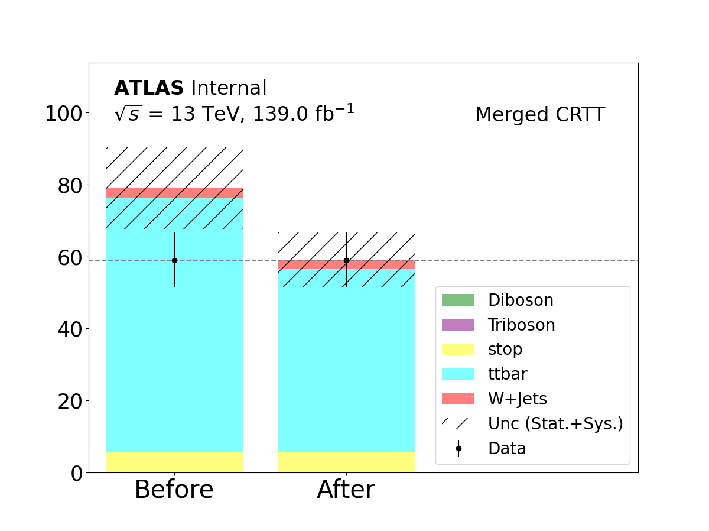
\includegraphics[width=\textwidth]{Figures/8/CRTT_Merged_before_after.pdf}
    \caption{Merged CRTT}\label{fig:before_after_CRTT_merged}
  \end{subfigure} \hspace{1em}
  \begin{subfigure}{0.45\textwidth}
    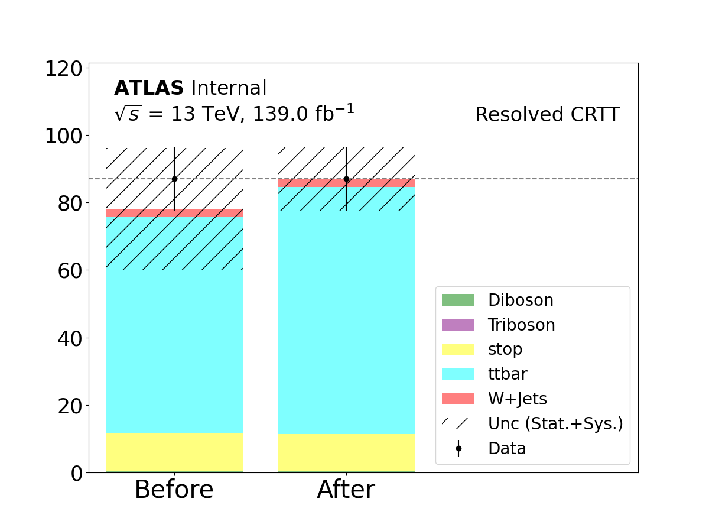
\includegraphics[width=\textwidth]{Figures/8/CRTT_Resolved_before_after.pdf}
    \caption{Resolved CRTT}\label{fig:before_after_CRTT_resolved}
  \end{subfigure} \\ \vspace{1em}
  \caption[]{Comparison between the predicted yields of SM background processes and observed yields of ATLAS collision data in the CRs, before and after the background-only fit. Hatched band shows the combined statistical and systematic uncertainty of the total yield prediction of SM background processes. Black error bars represent the Poisson uncertainty associated with the observed event count in each CR.}
  \label{fig:before_after_CRs}
\end{figure}

\subsection{Nuisance Parameter Pulls and Correlations}

Figure \ref{fig:pull_bkgonly} summarizes the post-fit shifts (a.k.a. ``pulls") of the values of all NPs included in the background-only fit, as well as their post-fit uncertainties. Both the values and uncertainties of the \(\boldsymbol{\mu}\) normalization factors, which scale the \wjets and \ttbar backgrounds separately in the merged and resolved categories, are constrained by the fit to obtain the post-fit agreement seen in Figure \ref{fig:before_after_CRs} between the total predicted yield of SM background processes and the observed yields in the ATLAS collision data. The values of all other NPs, which parametrize sources of statistical and systematic uncertainty, receive negligible pulls in the fit, since agreement with data can be obtained in all CRs just by varying the \wjets and \ttbar normalization factors. The uncertainties of the \(\gamma\)\_* parameters\footnote{See Table \ref{tab:np_naming} for a description of the scheme used to name NPs.} that parametrize the statistical uncertainty associated with the MC simulated yield predictions in each CR are reduced by the fit to data, which results in the reduction seen in Figure \ref{fig:before_after_CRs} of the uncertainty associated with the post-fit expected yield of SM background events.

\begin{figure}[h]
  \centering
  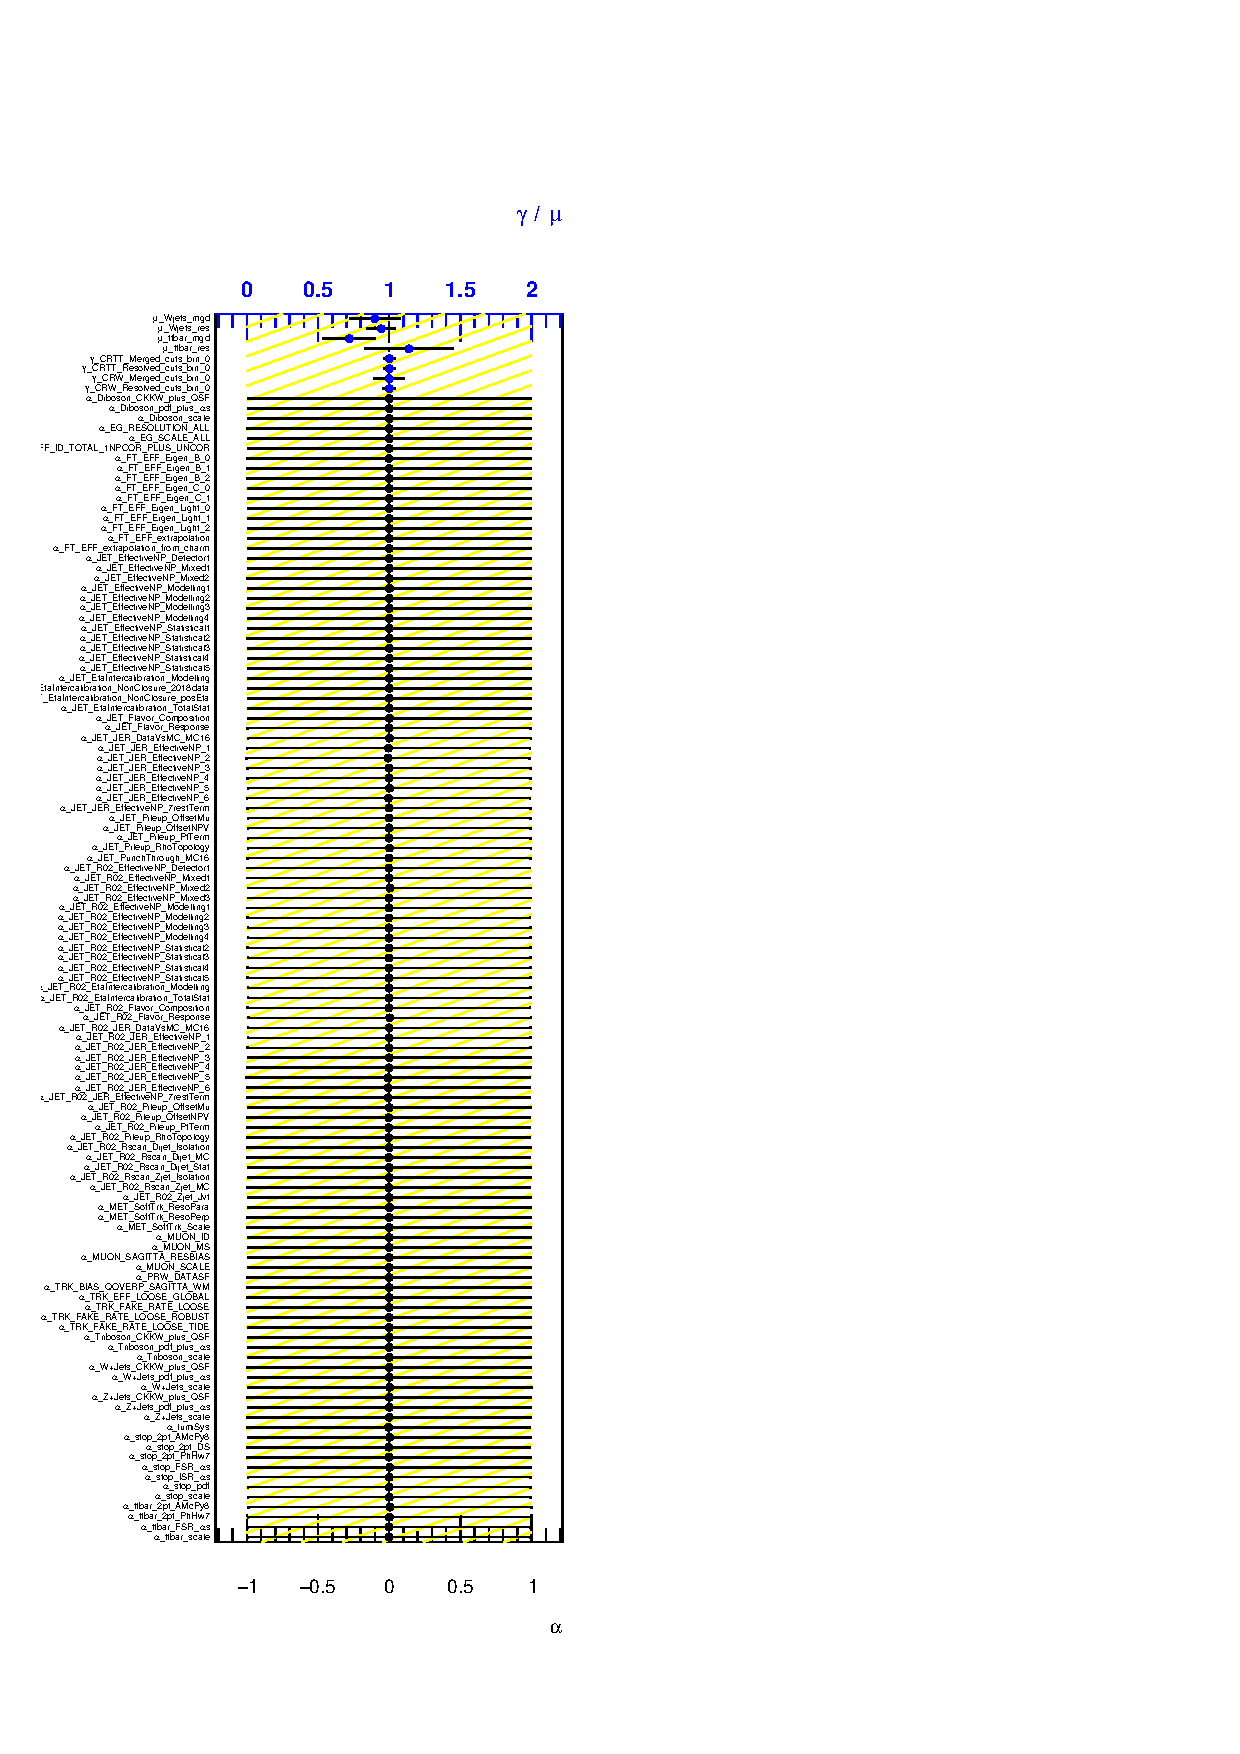
\includegraphics[width=0.55\textwidth]{Figures/8/BkgOnly/fit_parameters.pdf}
  \caption[Pull plots for background-only fit]{\footnotesize{Post-fit values and uncertainties of all NPs in the background-only fit. See Tables \ref{tab:np_naming}, \ref{tab:exp_syst_naming} and \ref{tab:theo_syst_naming} for details of the scheme used to name the NPs. Yellow hatched band shows the pre-fit uncertainty for each NP, and black horizontal error bars show the post-fit uncertainty.}}
  \label{fig:pull_bkgonly}
\end{figure}

Figure \ref{fig:corrs_bkgonly} shows the Pearson correlation coefficient \(r\) between NPs in the fit. There is some appreciable correlation (\(|r|\gtrsim0.2\)) between separate background normalization factors \(\mu\)\_*, and between normalization factors and a few of the \(\gamma\)\_* NPs - for example, \(r=-0.7\) between \(\mu\_\text{Wjets\_mgd}\) and \(\gamma\_\text{stat\_CRW\_Merged\_cuts\_bin\_0}\). However, there is in general very little cross correlation (\(r<0.01\)) between the \(\gamma\)\_* and \(\alpha\)\_* NPs, which collectively parametrize all uncertainty sources in the fit due to the negligible shifts induced on these parameters by the background-only fit (see Figure \ref{fig:pull_bkgonly}).

\begin{figure}[h]
  \centering
  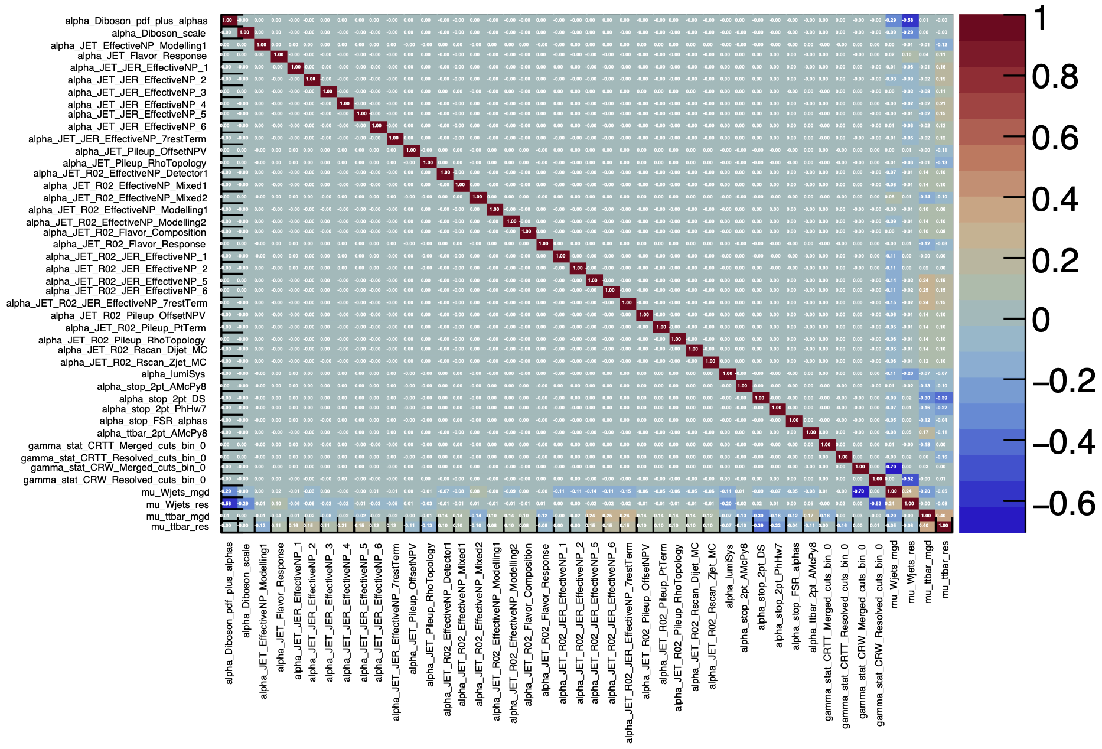
\includegraphics[width=\textwidth]{Figures/8/BkgOnly/c_corrMatrix_RooExpandedFitResult_afterFit_edited.pdf}
  \caption[Pull plots for background-only fit]{\footnotesize{Correlation matrix for all NPs considered in the background-only fit for which at least one coefficient of cross-correlation with another NP is larger than 0.1. See Tables \ref{tab:np_naming}, \ref{tab:exp_syst_naming} and \ref{tab:theo_syst_naming} for details of the scheme used to name the NPs.}}
  \label{fig:corrs_bkgonly}
\end{figure}

\section{Comparison of SM Background Expectation and Data in the Signal Region}

After performing the background-only fit in the CRs, the constraints on the background normalization factors \(\boldsymbol{\mu}\) and the other NPs \(\boldsymbol{\theta}\) summarized in Figure \ref{fig:pull_bkgonly} are extrapolated to the SR following the procedure described in Section \ref{sec:extrapolation}. Figure \ref{fig:before_after_SRs} compares the predicted yields of SM background processes in the SR - binned in \minms using the binning strategy presented in Section \ref{sec:binning_strategy} - before and after the background-only fit and extrapolation procedure. Table \ref{tab:pre_post_yields_SR} summarizes the total predicted and observed yields in the merged SRs, combined over all bins within each SR.

Both before and after the background-only fit extrapolation, Figures \ref{fig:before_SR_merged} and \ref{fig:after_SR_merged}, respectively, show an excess of observed ATLAS collision events compared with the predicted yield of SM background processes in the first three bins of the merged SR. However, the difference is within uncertainty in all three bins, and a comparison of the combined yields reported in the first row of Table \ref{tab:pre_post_yields_SR} reveals that the overall yield of ATLAS collision data in the merged SR a factor of 1.3 larger than the total post-fit uncertainty associated with the expected yield of SM background processes (a.k.a. a 1.3\(\sigma\) excess). If the distribution of measured discrepancies between the predicted yield of SM background processes and the observed yield of collision data is assumed to be reasonably approximated as Gaussian, the observed 1.3\(\sigma\) discrepancy corresponds to a two-sided p-value of 0.18 (see, for example, Section 11 of \cite{Stats_2003} for an introduction to the p-value and its use in hypothesis testing). If a p-value below 0.05 is taken to represent a statistically significant deviation from the null hypothesis, the observed p-value of 0.18 implies that the observed yield of ATLAS collision events in the merged SR is statistically compatible with the null hypothesis that all events observed in the SR were produced by SM background processes. 

%\begin{equation}
%\label{eq:merged_sigma}
%\frac{ \sum_{\text{bin }i\in\{\text{merged SR (S)}\}}\big[n_{S,i} - \lambda_{S,i, \text{ post-fit }}(\mu_\text{Sig}=0, \boldsymbol{\mu_i}, s_i, \boldsymbol{b_i}, \boldsymbol{\theta})\big] }{\sigma\Big(\sum_{\text{bin }i\in\{\text{merged SR (S)}\}} \lambda_{S,i}(\mu_\text{Sig}=0, \boldsymbol{\mu_i}, s_i, \boldsymbol{b_i}, \boldsymbol{\theta}) \Big)} = 1.3
%\end{equation}
%
%where \(n_{S,i}\) is the number of ATLAS collision events observed in bin \(i\) of the merged SR, \(\lambda_{S,i, \text{ post-fit }}(\mu_\text{Sig}=0, \boldsymbol{\mu_i}, s_i, \boldsymbol{b_i}, \boldsymbol{\theta})\) is the Poisson expectation defined in Eq. \ref{eq:lambda} for the total yield of MC background events in bin \(i\), assuming no signal content (\(\mu_\text{Sig}=0\)), and using values of the NPs \(\boldsymbol{\mu_i}\) and \(\boldsymbol{\theta}\) constrained in the background-only fit. \(\sigma\Big(\sum_{\text{bin }i\in\{\text{merged SR (S)}\}} \lambda_{S,i}(\mu_\text{Sig}=0, \boldsymbol{\mu_i}, s_i, \boldsymbol{b_i}, \boldsymbol{\theta}) \Big)\) is the total  uncertainty associated with the total post-fit yield expectation of SM background events in the merged SR, combined over all bins. If the ratio evaluated in Eq. \ref{eq:merged_sigma} is assumed to be sampled from a Gaussian parent distribution centred at 0 with standard deviation \(\sigma\Big(\sum_{\text{bin }i\in\{\text{merged SR (S)}\}} \lambda_{S,i}(\mu_\text{Sig}=0, \boldsymbol{\mu_i}, s_i, \boldsymbol{b_i}, \boldsymbol{\theta}) \Big)\), 

Figures \ref{fig:before_SR_resolved} and \ref{fig:after_SR_resolved} show an over-prediction of the SM background yield compared with the observed number of ATLAS collision events in all bins of the resolved SR, both before and after NP constraints from the background-only fit are extrapolated to the SRs. Comparing the observed yield of collision events from Table \ref{tab:pre_post_yields_SR} in the resolved SR with the post-fit predicted yield of SM background events reveals a \(-0.8\sigma\) discrepancy. The resulting two-sided Gaussian p-value of 0.42 indicates that, as in the merged SR, the observed yields are statistically compatible with the null background-only hypothesis. 

\begin{figure}[h]
  \centering
  \begin{subfigure}{0.45\textwidth}
    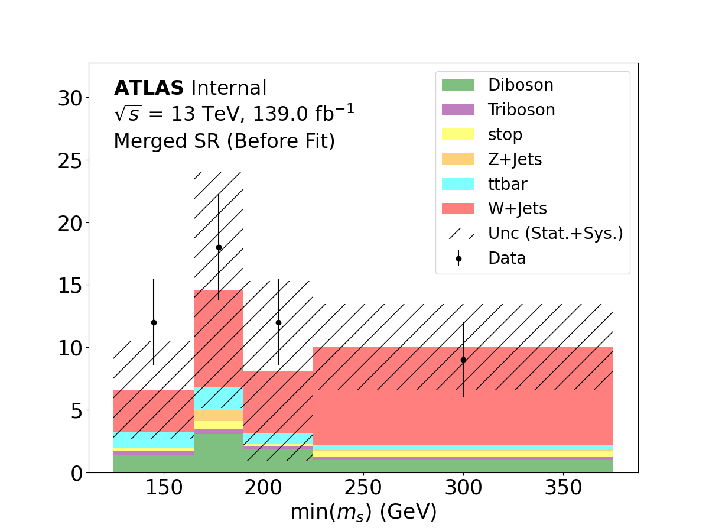
\includegraphics[width=\textwidth]{Figures/8/SR_Merged_before.pdf}
    \caption{Merged SR (Before Fit)}\label{fig:before_SR_merged}
  \end{subfigure} \hspace{1em}
  \begin{subfigure}{0.45\textwidth}
    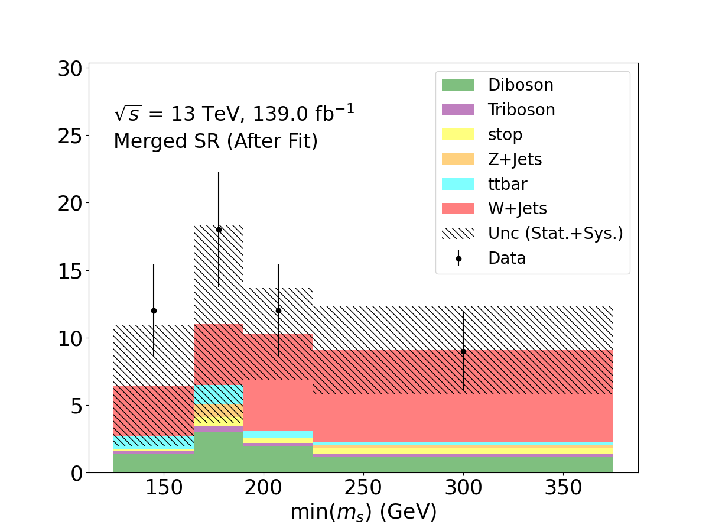
\includegraphics[width=\textwidth]{Figures/8/SR_Merged_after.pdf}
    \caption{Merged SR (After Fit)}\label{fig:after_SR_merged}
  \end{subfigure} \vspace{1em}
  \begin{subfigure}{0.45\textwidth}
    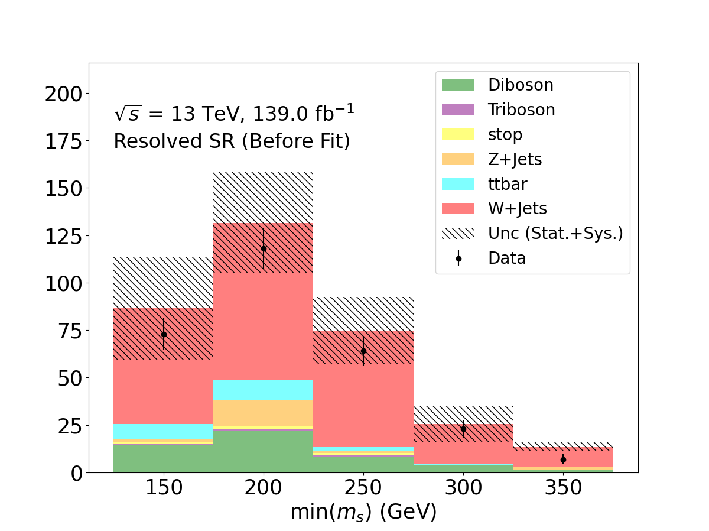
\includegraphics[width=\textwidth]{Figures/8/SR_Resolved_before.pdf}
    \caption{Resolved SR (Before Fit)}\label{fig:before_SR_resolved}
  \end{subfigure} \hspace{1em}
  \begin{subfigure}{0.45\textwidth}
    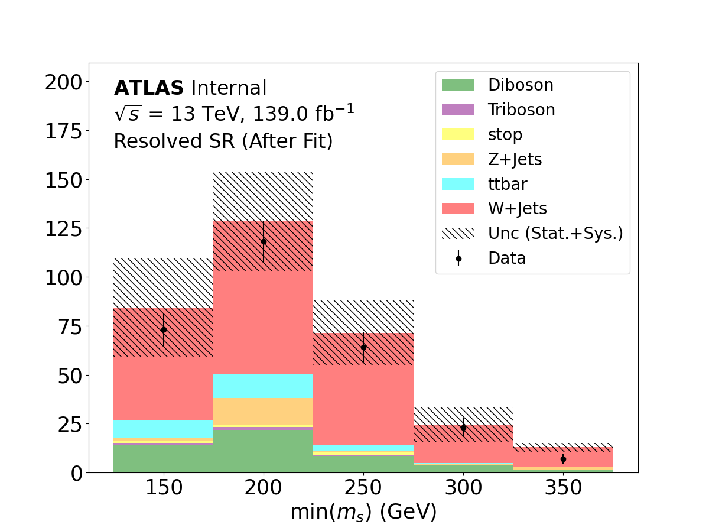
\includegraphics[width=\textwidth]{Figures/8/SR_Resolved_after.pdf}
    \caption{Resolved SR (After Fit)}\label{fig:after_SR_resolved}
  \end{subfigure} \\ \vspace{1em}
  \caption[]{Comparison between predicted yields of SM background processes and observed yields in the SRs, before (left) and after (right) the background-only fit and extrapolation to the SR. Yields are binned in \minms using the binning strategy presented in Section \ref{sec:binning_strategy}.}
  \label{fig:before_after_SRs}
\end{figure}

\begin{table}
\centering
\caption{Comparison of the total observed yields of events in the SRs with the predicted yield of SM background processes, either before (pre-fit) or after (post-fit) extrapolation of constraints from the background-only fit in the CRs.}
\label{tab:pre_post_yields_SR}
\begin{tabular}{l l l l}
\toprule
\textbf{Region} & \textbf{Observed Yield} & \textbf{SM Bkg Prediction} & \textbf{SM Bkg Prediction} \\
 & & \textbf{(Pre-fit)} & \textbf{(Post-fit)} \\
\midrule
\midrule
Merged SR & 51 & $39.7 \pm 11$ & $36.8 \pm 10$ \\
\midrule
Resolved SR & 285 & $331.7\pm 65$ & $321.2 \pm 40$ \\
\bottomrule
\end{tabular}
\end{table}

\section{Exclusion of the Dark Higgs Signal Model}

Given the absence of any statistically significant discrepancy between the observed yields of ATLAS collision events in the SRs and the predicted yields of events from SM background processes, the exclusion hypothesis test presented in Section \ref{sec:hypo_test} is used to determine the range of \ms and \mZp for which the DH signal model can be confidently excluded by the search for the fixed choices of the DM mass \(\mchi\), mixing angle \(\sin\theta\) and coupling choices \(g_q\) and \(\gchi\) in the DH model used for the search\footnote{See Sections \ref{sec:dh_model_free_parameters} and \ref{sec:dh_searches} for a presentation and discussion of the choices for the \mchi, \(\sin\theta\) and coupling parameters in the DH model.}:

\begin{itemize}
\item \(\mchi=200~\GeV\)
\item \(g_q=0.25\)
\item \(g_\chi=1\)
\item \(\sin\theta=0.01\)
\end{itemize}

\subsection{Signal+Background Fit}

Figures \ref{fig:before_after_SRs_MonoSlep_monoSWWsemilep_zp1000_dm200_dh160}, \ref{fig:before_after_SRs_MonoSlep_monoSWWsemilep_zp2100_dm200_dh210} and \ref{fig:before_after_SRs_MonoSlep_monoSWWsemilep_zp2900_dm200_dh310} compare the observed yield of ATLAS collision events in the SRs, binned in \minms, with the predicted yields for the SM background and DH signal processes at the three sample combinations of \ms and \mZp in the signal model. The sample \ms and \mZp combinations, listed below, are chosen to cover the range of production cross sections for the DH model considered in the search:

\begin{itemize}
\item \((\ms, \mZp) = (160, 1000)~\GeV\) (cross section: 93.3 fb\(^{-1}\))
\item \((\ms, \mZp) = (210, 2100)~\GeV\) (cross section: 3.9 fb\(^{-1}\))
\item \((\ms, \mZp) = (310, 2900)~\GeV\) (cross section: 0.31 fb\(^{-1}\))
\end{itemize}

As shown in Figure \ref{fig:before_after_SRs_MonoSlep_monoSWWsemilep_zp1000_dm200_dh160}, the DH signal model at \((\ms, \mZp) = (160, 1000)~\GeV\) with a cross section of 93.3 fb\({^{-1}}\) has a sufficiently large production rate that the signal+background fit constrains the signal strength parameter to \(\mu_\text{Sig}=0.09\pm0.08\). Therefore, the signal+background hypothesis (\(\mu_\text{Sig}=1\)) is excluded with a high degree of confidence.

Figure \ref{fig:before_after_SRs_MonoSlep_monoSWWsemilep_zp2100_dm200_dh210} shows the results of the signal+background fit for \((\ms, \mZp) = (210, 2100)~\GeV\) in the signal model, with an intermediate cross section of 3.9 fb\(^{-1}\). The predicted yield of the signal process is comparable in the first three bins of the merged SR to the discrepancy between the observed yield of data and the predicted yield of SM background processes, which results in a fitted signal strength close to 1 (\(\mu_\text{Sig}=0.88\)). However, since the predicted yield of the signal and background processes are still consistent with the background-only prediction, there is a large (nearly 100\%) uncertainty associated with the fitted signal strength. As a result, the fit can neither support nor confidently exclude the signal+background hypothesis at this mass point. 

Further reduced exclusion power is observed for the fit shown in Figure \ref{fig:after_SR_merged_MonoSlep_monoSWWsemilep_zp2900_dm200_dh310}, which considers the signal model at the mass combination \((\ms, \mZp) = (310, 2900)~\GeV\) with the lowest cross section of the three combinations considered. The signal yields are so small compared with the uncertainty of the total yield prediction that the fitted signal strength could range from \(-3.82\) to \(5.06\) within its post-fit uncertainty. As a result, the search can neither meaningfully support nor exclude the DH signal model at this mass point.

\begin{figure}[h]
  \centering
  \begin{subfigure}{0.45\textwidth}
    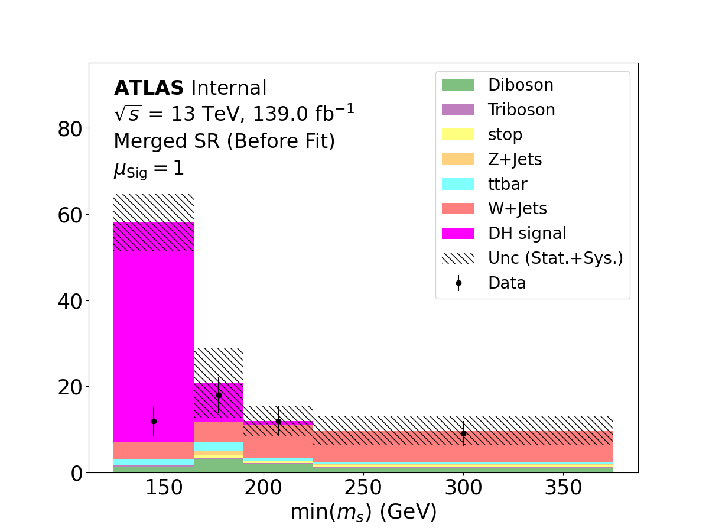
\includegraphics[width=\textwidth]{Figures/8/MonoSlep_monoSWWsemilep_zp1000_dm200_dh160/SR_Merged_before.pdf}
    \caption{Merged SR (Before Fit)}\label{fig:before_SR_merged_MonoSlep_monoSWWsemilep_zp1000_dm200_dh160}
  \end{subfigure} \hspace{1em}
  \begin{subfigure}{0.45\textwidth}
    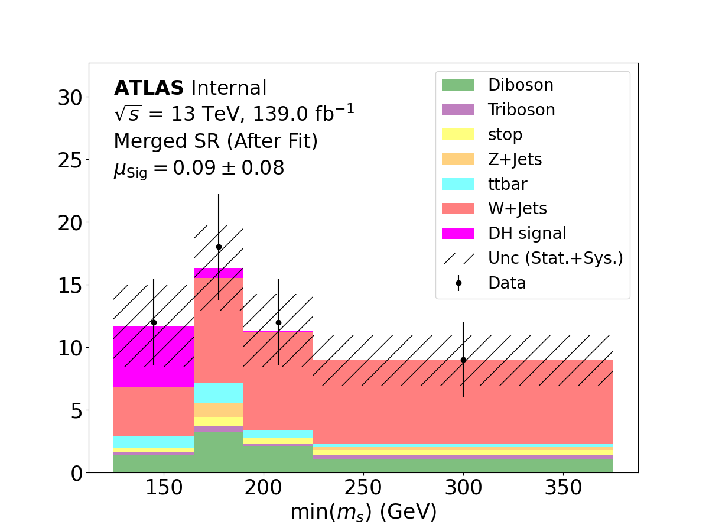
\includegraphics[width=\textwidth]{Figures/8/MonoSlep_monoSWWsemilep_zp1000_dm200_dh160/SR_Merged_after.pdf}
    \caption{Merged SR (After Fit)}\label{fig:after_SR_resolved_MonoSlep_monoSWWsemilep_zp1000_dm200_dh160}
  \end{subfigure} \vspace{1em}
  \begin{subfigure}{0.45\textwidth}
    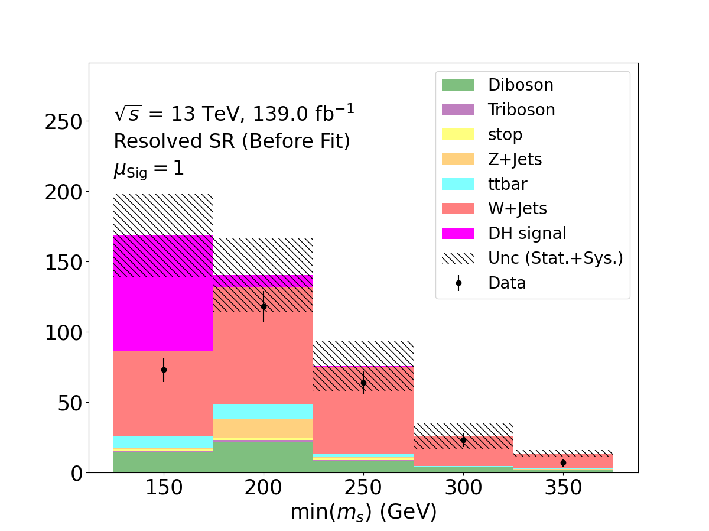
\includegraphics[width=\textwidth]{Figures/8/MonoSlep_monoSWWsemilep_zp1000_dm200_dh160/SR_Resolved_before.pdf}
    \caption{Resolved SR (Before Fit)}\label{fig:before_SR_merged_MonoSlep_monoSWWsemilep_zp1000_dm200_dh160}
  \end{subfigure} \hspace{1em}
  \begin{subfigure}{0.45\textwidth}
    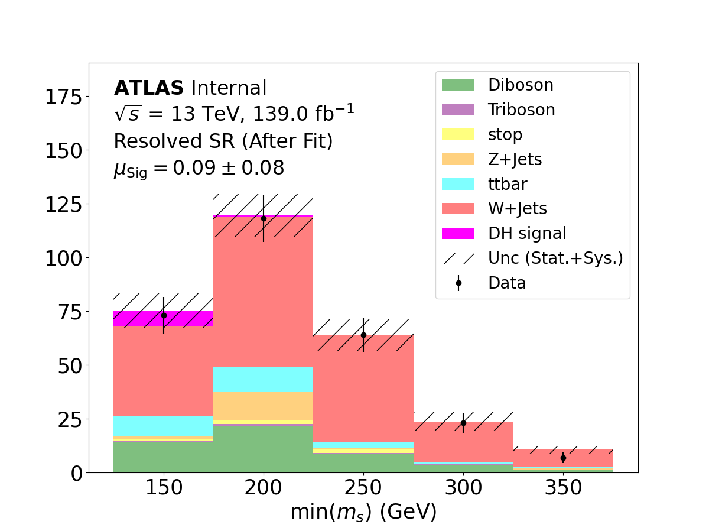
\includegraphics[width=\textwidth]{Figures/8/MonoSlep_monoSWWsemilep_zp1000_dm200_dh160/SR_Resolved_after.pdf}
    \caption{Resolved SR (After Fit)}\label{fig:after_SR_merged_MonoSlep_monoSWWsemilep_zp1000_dm200_dh160}
  \end{subfigure} \\ \vspace{1em}
  \caption[]{Comparison between predicted yields of SM background processes, the DH signal process at \((\ms, \mZp) = (160, 1000)~\GeV\) and observed yields in the SRs. Yields are shown before (left) and after (right) the signal+background fit. The pre-and post-fit values of the signal strength \(\mu_\text{Sig}\) are also reported. Yields are binned in \minms using the binning strategy presented in Section \ref{sec:binning_strategy}.}
  \label{fig:before_after_SRs_MonoSlep_monoSWWsemilep_zp1000_dm200_dh160}
\end{figure}

\begin{figure}[h]
  \centering
  \begin{subfigure}{0.45\textwidth}
    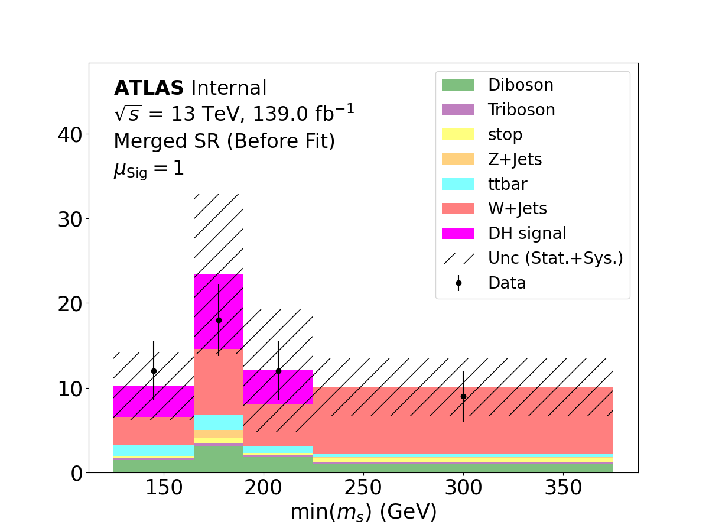
\includegraphics[width=\textwidth]{Figures/8/MonoSlep_monoSWWsemilep_zp2100_dm200_dh210/SR_Merged_before.pdf}
    \caption{Merged SR (Before Fit)}\label{fig:before_SR_merged_MonoSlep_monoSWWsemilep_zp2100_dm200_dh210}
  \end{subfigure} \hspace{1em}
  \begin{subfigure}{0.45\textwidth}
    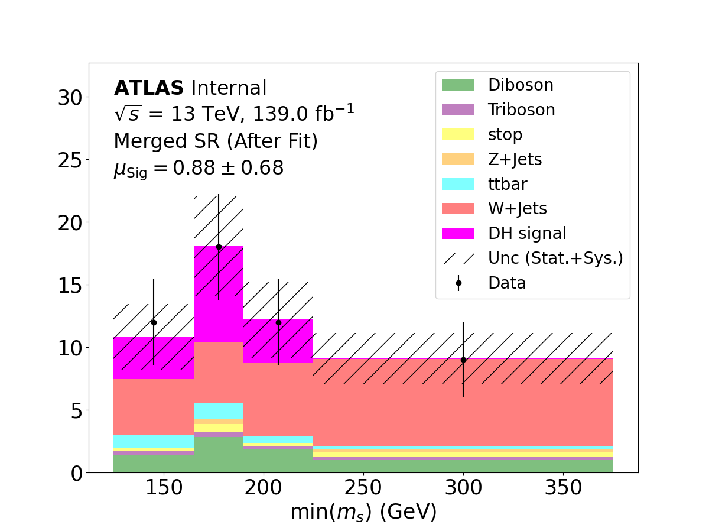
\includegraphics[width=\textwidth]{Figures/8/MonoSlep_monoSWWsemilep_zp2100_dm200_dh210/SR_Merged_after.pdf}
    \caption{Merged SR (After Fit)}\label{fig:after_SR_resolved_MonoSlep_monoSWWsemilep_zp2100_dm200_dh210}
  \end{subfigure} \vspace{1em}
  \begin{subfigure}{0.45\textwidth}
    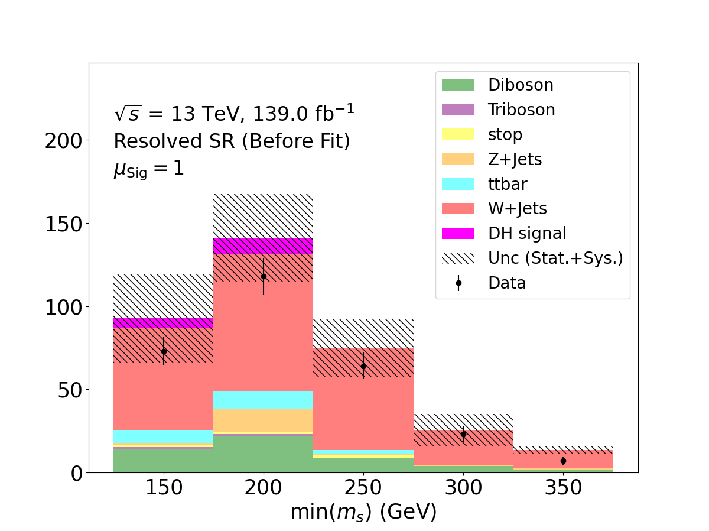
\includegraphics[width=\textwidth]{Figures/8/MonoSlep_monoSWWsemilep_zp2100_dm200_dh210/SR_Resolved_before.pdf}
    \caption{Resolved SR (Before Fit)}\label{fig:before_SR_merged_MonoSlep_monoSWWsemilep_zp2100_dm200_dh210}
  \end{subfigure} \hspace{1em}
  \begin{subfigure}{0.45\textwidth}
    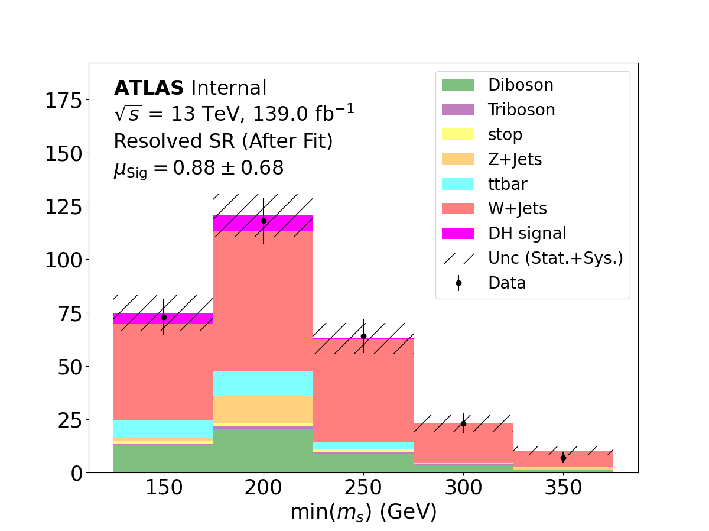
\includegraphics[width=\textwidth]{Figures/8/MonoSlep_monoSWWsemilep_zp2100_dm200_dh210/SR_Resolved_after.pdf}
    \caption{Resolved SR (After Fit)}\label{fig:after_SR_merged_MonoSlep_monoSWWsemilep_zp2100_dm200_dh210}
  \end{subfigure} \\ \vspace{1em}
  \caption[]{Comparison between predicted yields of SM background processes, the DH signal process at \((\ms, \mZp) = (210, 2100)~\GeV\) and observed yields in the SRs. Yields are shown before (left) and after (right) the signal+background fit. The pre-and post-fit values of the signal strength \(\mu_\text{Sig}\) are also reported. Yields are binned in \minms using the binning strategy presented in Section \ref{sec:binning_strategy}.}
  \label{fig:before_after_SRs_MonoSlep_monoSWWsemilep_zp2100_dm200_dh210}
\end{figure}

\begin{figure}[h]
  \centering
  \begin{subfigure}{0.45\textwidth}
    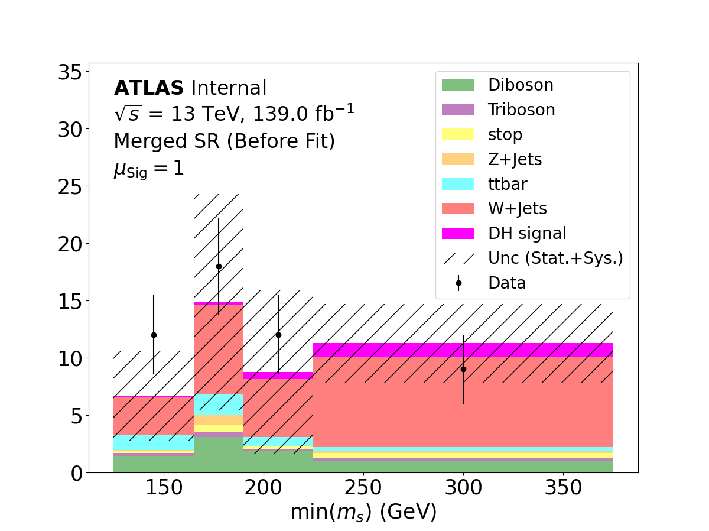
\includegraphics[width=\textwidth]{Figures/8/MonoSlep_monoSWWsemilep_zp2900_dm200_dh310/SR_Merged_before.pdf}
    \caption{Merged SR (Before Fit)}\label{fig:before_SR_merged_MonoSlep_monoSWWsemilep_zp2900_dm200_dh310}
  \end{subfigure} \hspace{1em}
  \begin{subfigure}{0.45\textwidth}
    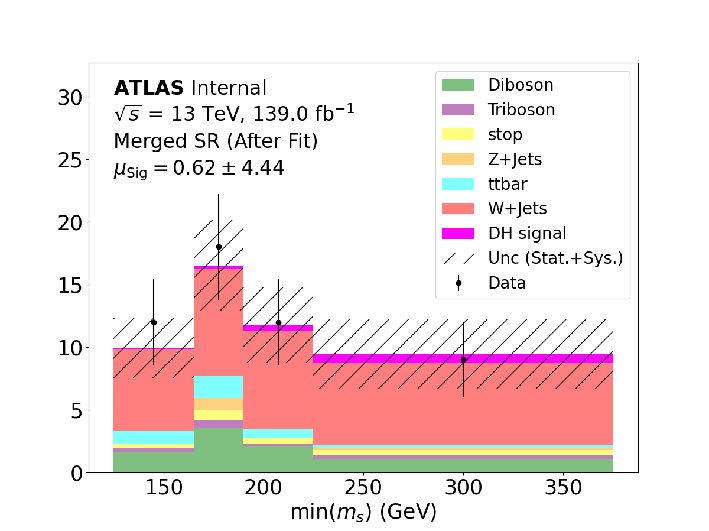
\includegraphics[width=\textwidth]{Figures/8/MonoSlep_monoSWWsemilep_zp2900_dm200_dh310/SR_Merged_after.pdf}
    \caption{Merged SR (After Fit)}\label{fig:after_SR_resolved_MonoSlep_monoSWWsemilep_zp2900_dm200_dh310}
  \end{subfigure} \vspace{1em}
  \begin{subfigure}{0.45\textwidth}
    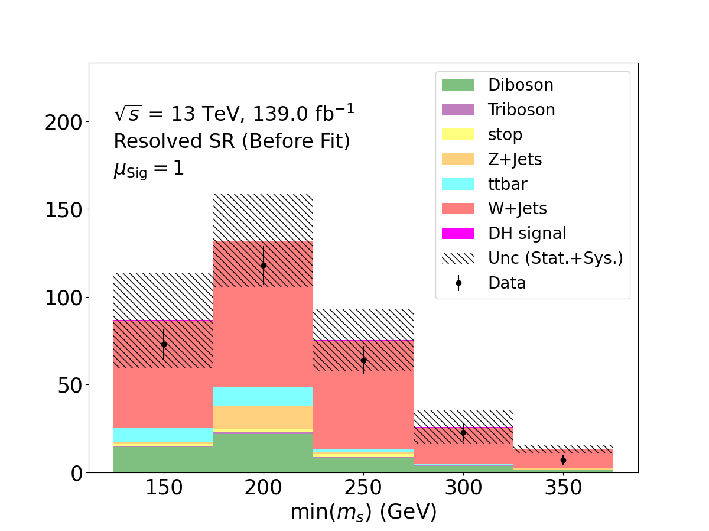
\includegraphics[width=\textwidth]{Figures/8/MonoSlep_monoSWWsemilep_zp2900_dm200_dh310/SR_Resolved_before.pdf}
    \caption{Resolved SR (Before Fit)}\label{fig:before_SR_merged_MonoSlep_monoSWWsemilep_zp2900_dm200_dh310}
  \end{subfigure} \hspace{1em}
  \begin{subfigure}{0.45\textwidth}
    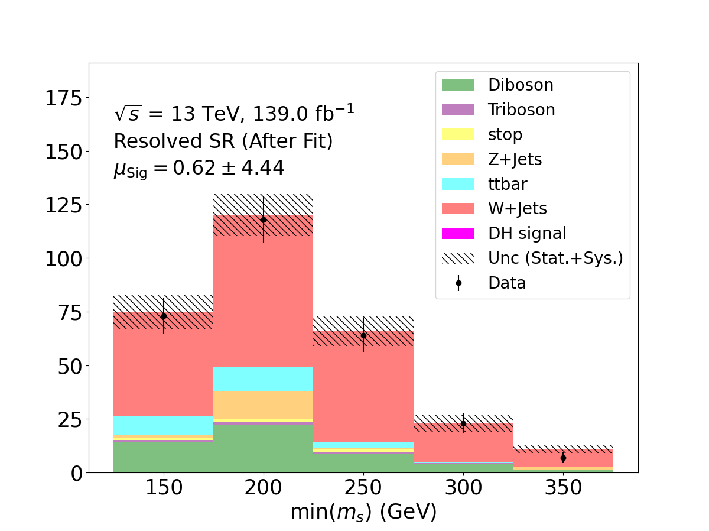
\includegraphics[width=\textwidth]{Figures/8/MonoSlep_monoSWWsemilep_zp2900_dm200_dh310/SR_Resolved_after.pdf}
    \caption{Resolved SR (After Fit)}\label{fig:after_SR_merged_MonoSlep_monoSWWsemilep_zp2900_dm200_dh310}
  \end{subfigure} \\ \vspace{1em}
  \caption[]{Comparison between predicted yields of SM background processes, the DH signal process at \((\ms, \mZp) = (310, 2900)~\GeV\) and observed yields in the SRs. Yields are shown before (left) and after (right) the signal+background fit. The pre-and post-fit values of the signal strength \(\mu_\text{Sig}\) are also reported. Yields are binned in \minms using the binning strategy presented in Section \ref{sec:binning_strategy}.}
  \label{fig:before_after_SRs_MonoSlep_monoSWWsemilep_zp2900_dm200_dh310}
\end{figure}

Figure \ref{fig:fitted_mu_Sig} summarizes the post-fit value and uncertainty of the signal strength parameter \(\mu_\text{Sig}\) for the signal+background fit performed with the DH signal model at all \ms and \mZp considered in the search. The fitted value and uncertainty vary depending on the production cross section and the shape of the signal distribution with respect to \minms. The size of the uncertainty for a given \ms and \mZp combination reflects the exclusion power of the search at the given mass combination, where a larger uncertainty generally implies less exclusion power. In general, the fitted values of \(\mu_\text{Sig}\) are consistent with 0 within 1.5\(\sigma\), in agreement with the null background-only hypothesis.

\begin{figure}[h]
  \centering
  \begin{subfigure}{0.49\textwidth}
    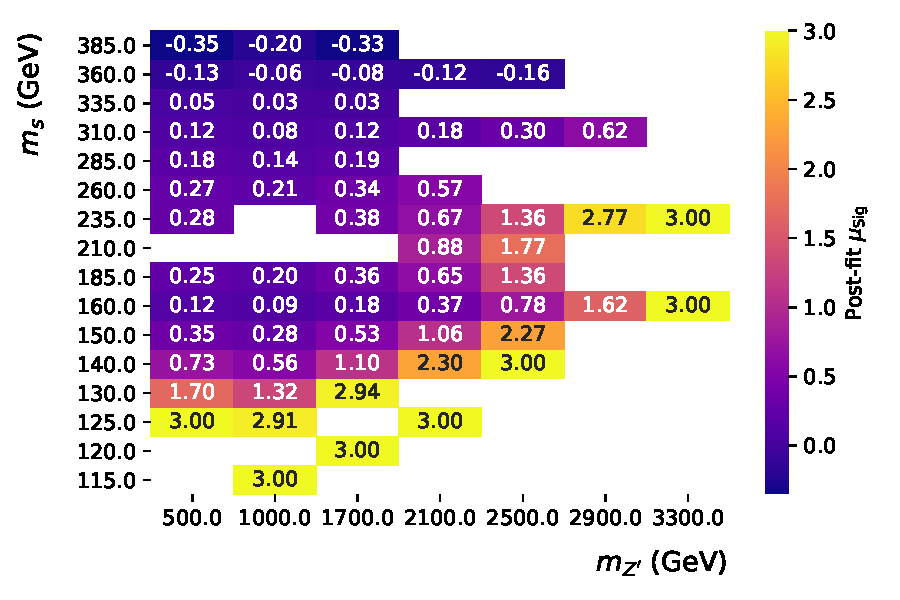
\includegraphics[width=\textwidth]{Figures/8/mu_sigs.pdf}
    \caption{Post-fit \(\mu_\text{Sig}\)}\label{fig:fitted_mu_Sig}
  \end{subfigure} 
  \begin{subfigure}{0.49\textwidth}
    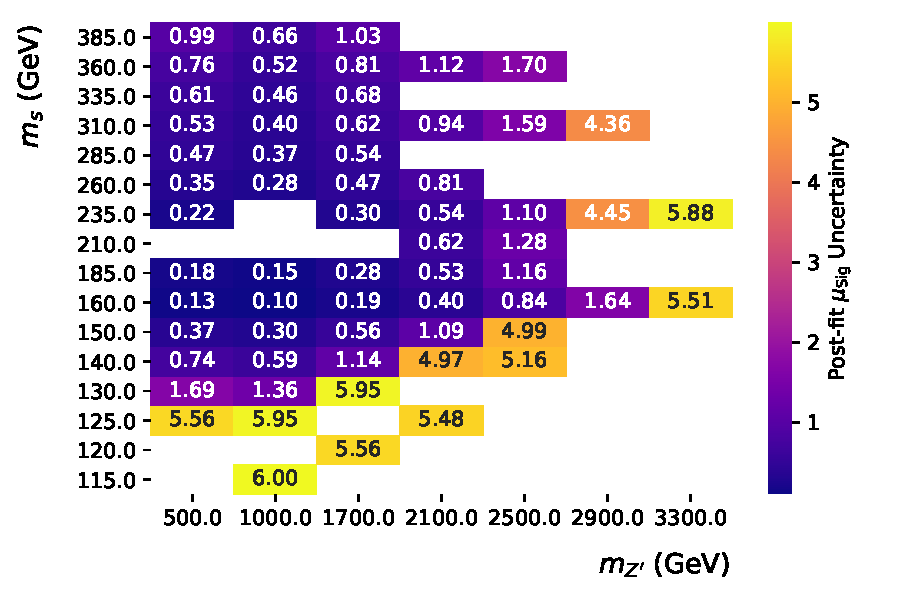
\includegraphics[width=\textwidth]{Figures/8/mu_sig_unc.pdf}
    \caption{Post-fit \(\mu_\text{Sig}\) uncertainty}\label{fig:fitted_mu_Sig_unc}
  \end{subfigure} 
  \caption[]{Post-fit value (left) and uncertainty (right) of the signal strength parameter \(\mu_\text{Sig}\) in the signal+background fit (\(\mu_\text{Sig}\) left floating) for each \ms and \mZp in the DH signal model.}
  \label{fig:fitted_mu_Sig}
\end{figure}

\subsubsection{Nuisance Parameter Pulls and Correlations}
\label{sec:np_pulls_sig_plus_bkg}

Figure \ref{fig:pull_sigPlusBkg} summarizes the pulls and uncertainties of all NPs included in the signal+background fit using the DH signal model at the sample mass point \((\ms, \mZp) = (210, 2100)~\GeV\). In contrast with the background-only fit, the pulls of some \(\gamma\)\_* and \(\alpha\)\_* NPs, which constrain the statistical and systematic uncertainties associated with MC simulated yields, can be appreciably shifted (i.e. pulled) relative to their pre-fit values. This is due to differences in the shapes of \minms distributions in the SRs between the observed ATLAS collision data and the predicted yields of the SM background and signal processes, which cannot be corrected by varying the \(\mu\)\_* normalization parameters alone. Particularly large pulls are seen for the NPs \(\alpha\)\_JET\_JER\_* and \(\alpha\)\_JET\_R02\_JER\_*, which parametrize the systematic jet energy resolution (JER) uncertainties associated with the \(R=0.4\)\footnote{See Section \ref{sec:atk4_jets} for a description of the \(R=0.4\) jets, and Section \ref{sec:resolved_w_cand} for a description of the method used to reconstruct the \(W\) boson candidate in the resolved category.} and \(R=0.2\)\footnote{See Section \ref{sec:TAR_algo} for a description of the algorithm used to construct TAR jets using input \(R=0.2\) jets.}  jets, respectively (see Tables \ref{tab:exp_syst_naming} and \ref{tab:theo_syst_naming} for descriptions of individual NPs used to parametrize systematic uncertainties). As shown in Figures \ref{fig:exp_syst_shifts_bkg} and \ref{fig:exp_syst_shifts_sig}, the JER systematic uncertainties induce the largest yield shifts in the SRs relative to other systematic sources. Therefore, it is reasonable to expect that these NPs would in general receive relatively strong pulls in the signal+background fit to help correct for the observed differences between expected and observed event yields in the SRs. 

\begin{figure}[h]
  \centering
  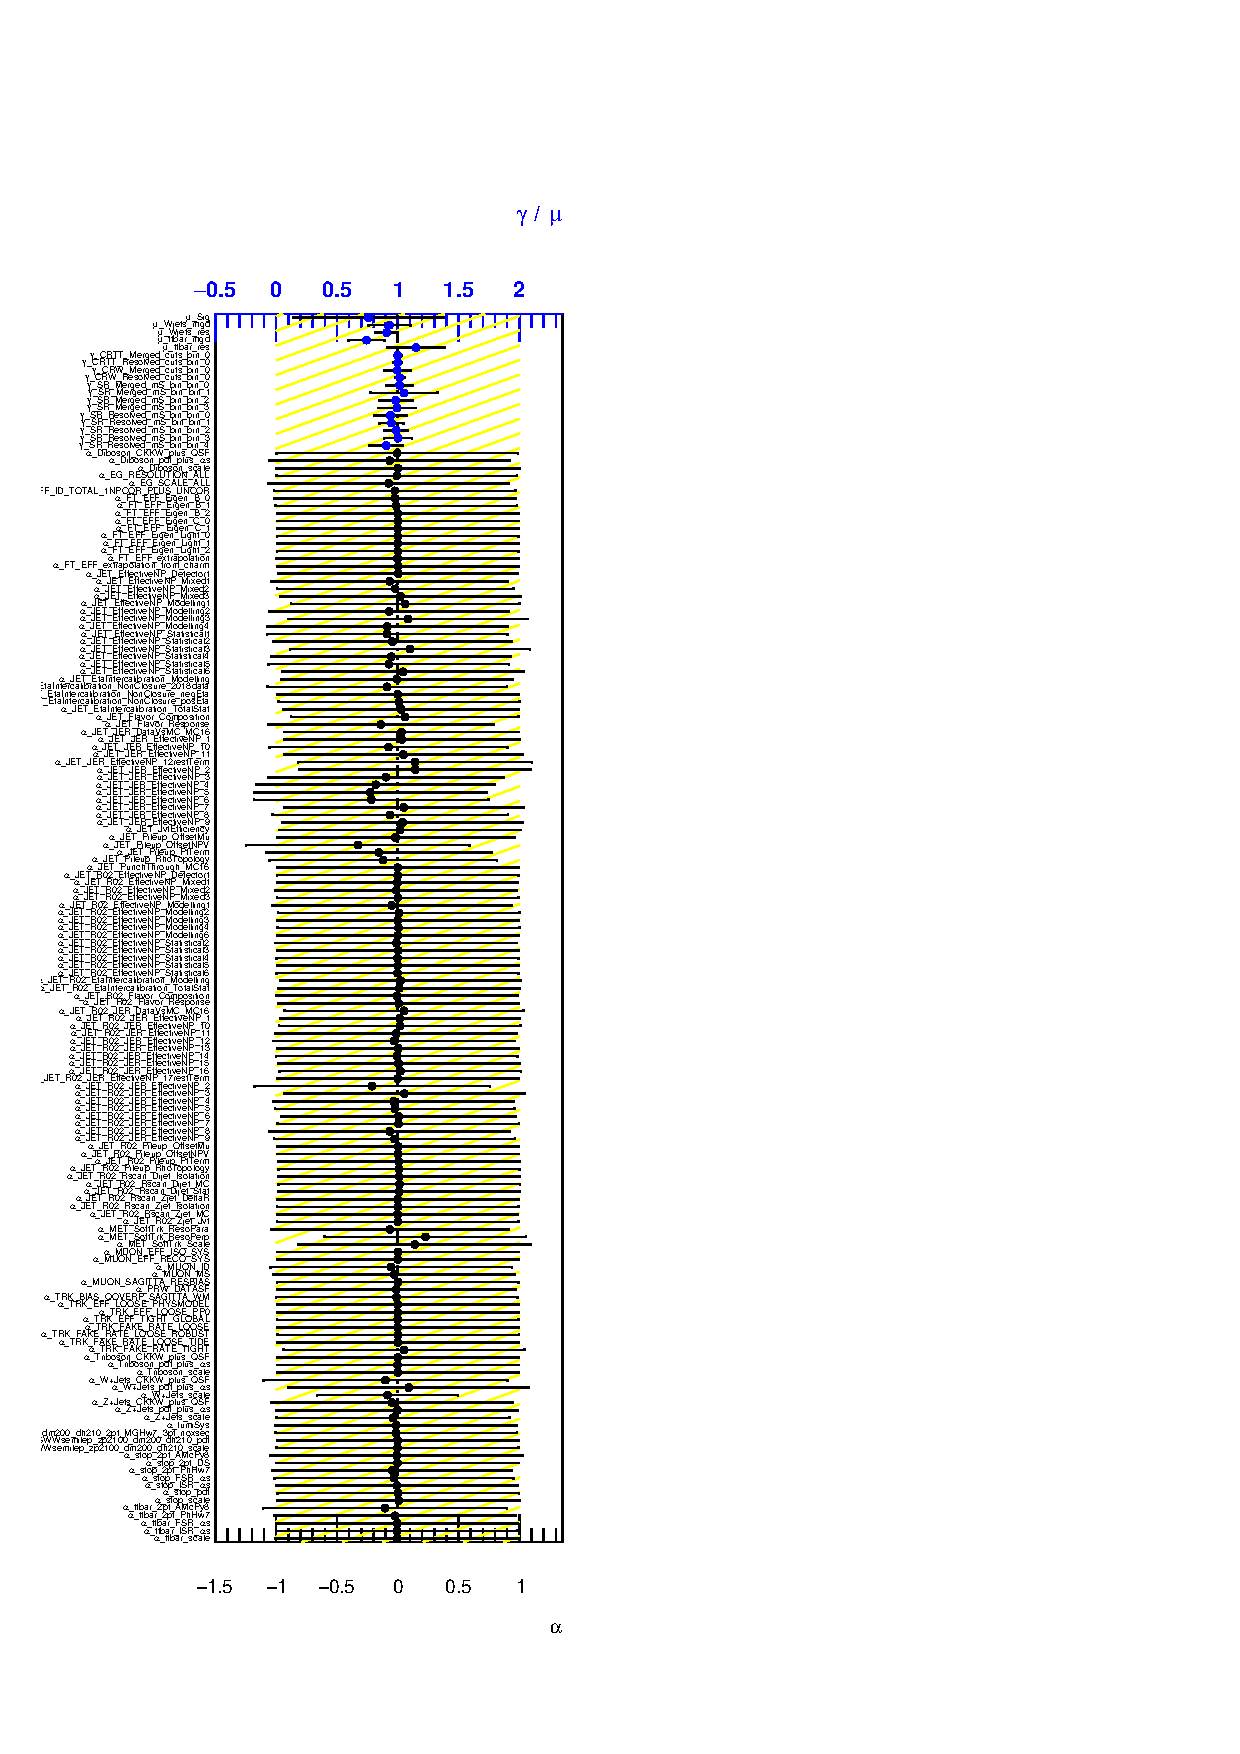
\includegraphics[width=0.5\textwidth]{Figures/8/MonoSlep_monoSWWsemilep_zp2100_dm200_dh210/fit_parameters.pdf}
  \caption[Pull plots for blinded SRs]{\footnotesize{Post-fit values of all NPs in the signal+background fit using the DH signal model at \((\ms, \mZp) = (210, 2100)~\GeV\). See Tables \ref{tab:np_naming}, \ref{tab:exp_syst_naming} and \ref{tab:theo_syst_naming} for details of the scheme used to name the NPs. Yellow hatched band shows the pre-fit uncertainty for each NP, and black horizontal error bars show the post-fit uncertainty.}}
  \label{fig:pull_sigPlusBkg}
\end{figure}

Figure \ref{fig:corrs_sigPlusBkg} shows the Pearson correlation coefficient \(r\) between NPs in the signal+background fit for the sample mass point \((\ms, \mZp) = (210, 2100)~\GeV\) in the DH signal model. As with the background-only fit, there is appreciable correlation (\(|r|\gtrsim0.2\)) between separate background normalization factors \(\mu\)\_*, and between normalization factors and several of the \(\gamma\)\_* NPs that parametrize the statistical uncertainties associated with MC simulated yield predictions. In contrast to the background-only fit, some of the \(\alpha\)\_* parameters also have non-negligible correlations (\(|r|\) up to \(\sim0.3\)) with one another and with \(\gamma\)\_* and \(\mu\)\_* NPs. The introduction of correlations involving \(\alpha\)\_* NPs in the signal+background fit compared with the background-only fit is attributed to the non-negligible post-fit shifts of these NPs observed in Figure \ref{fig:pull_sigPlusBkg} for the signal+background fit.

\begin{figure}[h]
  \centering
  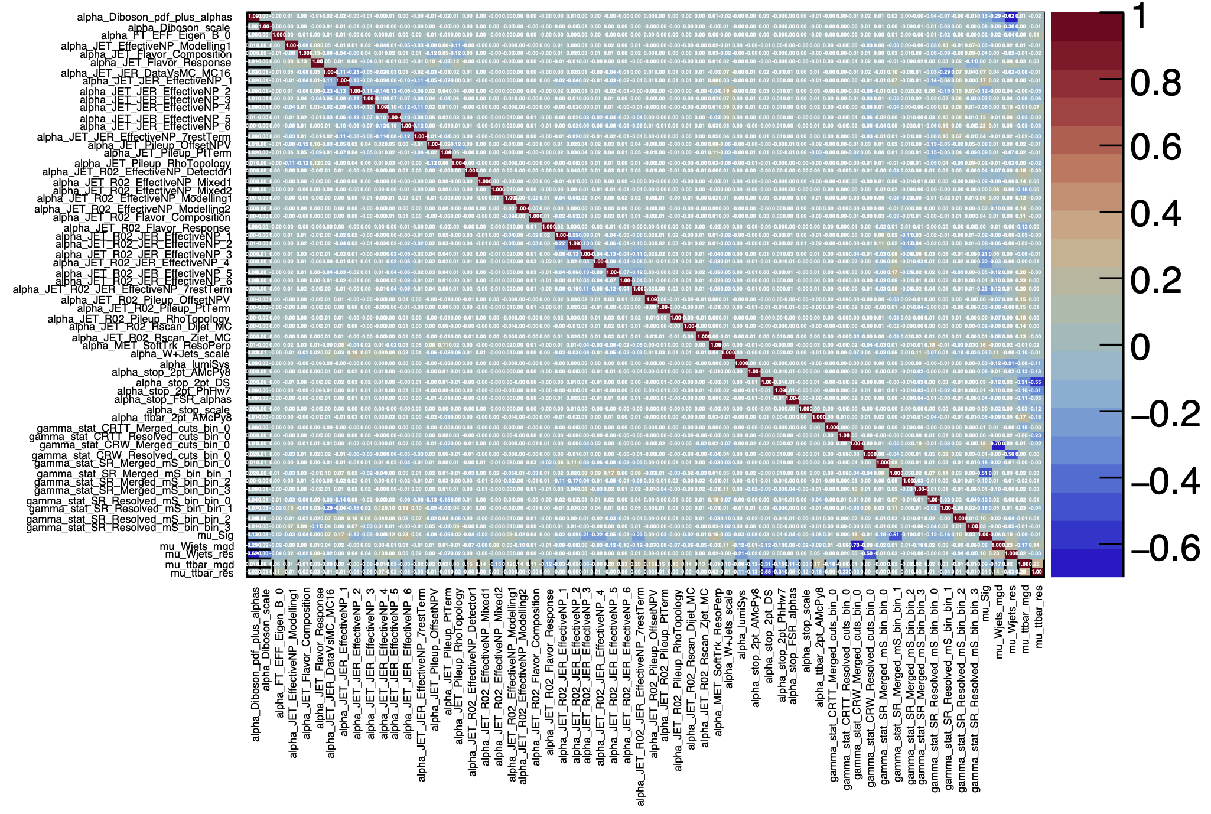
\includegraphics[width=\textwidth]{Figures/8/MonoSlep_monoSWWsemilep_zp2100_dm200_dh210/c_corrMatrix_RooExpandedFitResult_afterFit_edited.pdf}
  \caption[Pull plots for blinded SRs]{\footnotesize{Correlation matrix for all NPs considered in the signal+background fit at a sample signal point of \((\ms, \mZp) = (210, 2100)~\GeV\), for which at least one coefficient of cross-correlation with another NP is larger than 0.1. See Tables \ref{tab:np_naming}, \ref{tab:exp_syst_naming} and \ref{tab:theo_syst_naming} for details of the scheme used to name the NPs.}}
  \label{fig:corrs_sigPlusBkg}
\end{figure}

\subsubsection{Ranking of Systematic Uncertainties}

Figure \ref{fig:ranking_ms210} shows the pre- and post-fit values and impacts of NPs in the signal+background fit on the fitted signal strength \(\mu_\text{Sig}\). The 30 leading NPs are ranked from top to bottom in order of the size of their impact. The pre- and post-fit impact of a given NP \(\theta\) is measured as follows:

\begin{itemize}
    \item \textbf{Pre-fit impact:} Shift the value of \(\theta\) to the upper bound \(\theta_0+\Delta\theta\) of its pre-fit uncertainty. Perform the signal+background fit with \(\theta\) fixed to this upper value, and all other NPs left floating. Repeat with the value of \(\theta\) fixed to the lower bound \(\theta_0+\Delta\theta\) of its pre-fit uncertainty. The resulting shifts \(\Delta_\text{up/down}{\reallywidehat{\mu_\text{Sig}}}\) of the best-fit \(\mu_\text{Sig}\) are shown as unfilled white boxes with black borders in Figure \ref{fig:ranking_ms210}.
    \item \textbf{Post-fit impact:} As above, but with the value of \(\theta\) shifted instead to the upper and lower bounds of its post-fit uncertainty. The resulting shifts \(\Delta_\text{up/down}{\reallywidehat{\mu_\text{Sig}}}\) are shown as filled boxes, where the colour of the box indicates whether \(\mu_\text{Sig}\) is correlated (blue) or anti-correlated (green) with the value of the NP.
\end{itemize}

The highest-ranked NPs are associated with systematic JER uncertainties, which also receive some of the largest pulls in the fit (see Figure \ref{fig:pull_sigPlusBkg} and related discussion in Section \ref{sec:np_pulls_sig_plus_bkg}). Following in rank are some of the statistical \(\gamma\)\_* NPs. 

\begin{figure}[h]
  \centering
  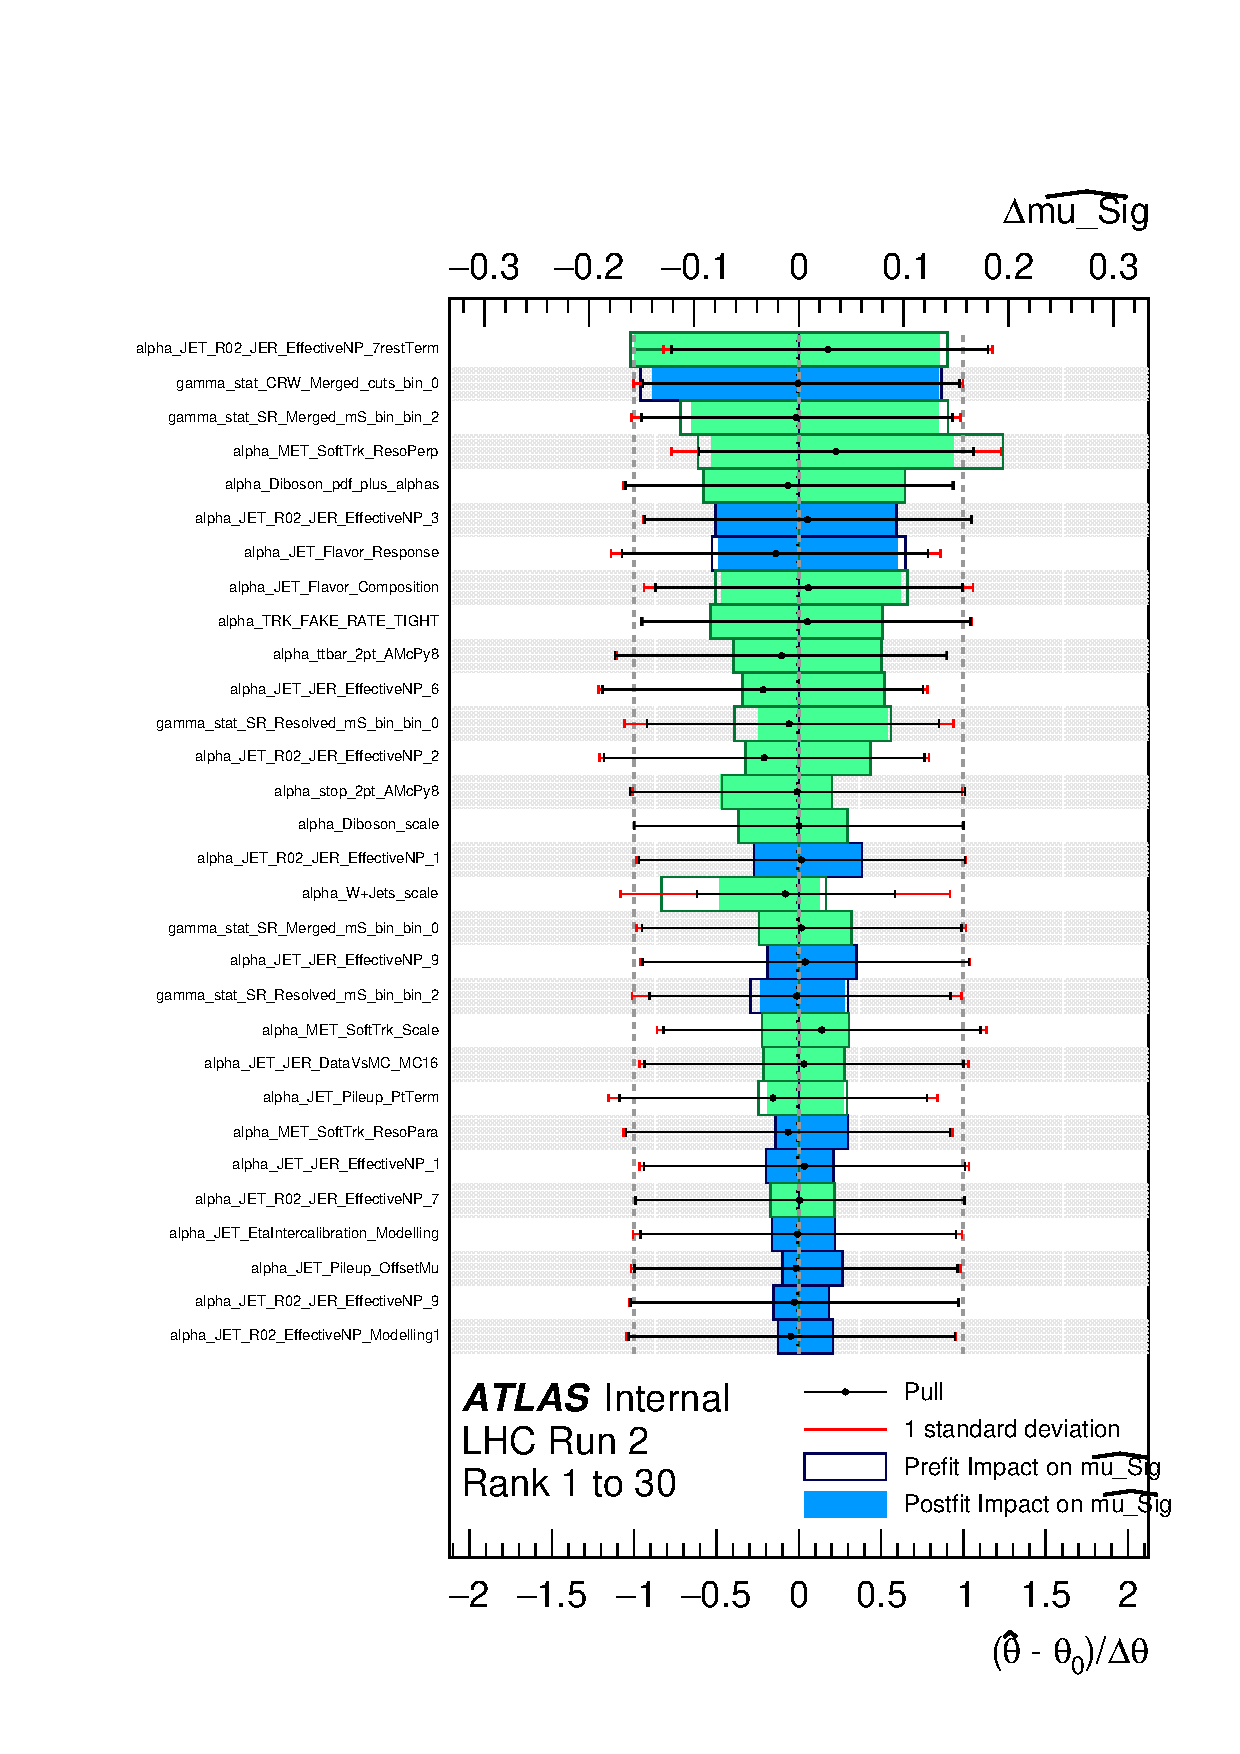
\includegraphics[width=0.9\textwidth]{Figures/8/ranking_mu_Sig_rank_0001_to_0030_zp2100_dm200_dh210_unblinded.pdf}
  \caption[Pre- and post-fit impacts for unblinded CRs (\ms, \mZp)=(210, 2100) GeV]{Leading 30 pre-and post-fit impacts on \(\mu_\text{Sig}\) for NPs associated with experimental and theoretical uncertainties in the signal+background fit at the sample signal point (\ms, \mZp)=(210, 2100) GeV. NPs are ranked from top to bottom in order of the size of their impact on \(\mu_\text{Sig}\). Blue (green) colouring of post-fit impacts indicates positive (negative) correlation with the signal strength. Post-fit values of the NPs (a.k.a. ``pulls") are also shown as black circles, where red (black) error bars show the size of the pre-fit (post-fit) uncertainty.}
  \label{fig:ranking_ms210}
\end{figure}

\subsection{Hypothesis Testing and Model Exclusion}

Hypothesis testing is performed following the method presented in Section \ref{sec:hypo_test} to determine the range of \ms and \mZp that can be confidently excluded by the search. The colour map in Figure \ref{fig:limits} shows the expected CL\(_s\) value evaluated over the range of \ms and \mZp considered in the search. Interpolated contours are drawn at CL\(_s=0.05\) for the expected (grey dashed) and observed (solid red) values, and the contained areas represent the expected and observed range of \ms and \mZp that are excluded by the search for the assumed DM mass and coupling choices.

\begin{figure}[h]
  \centering
  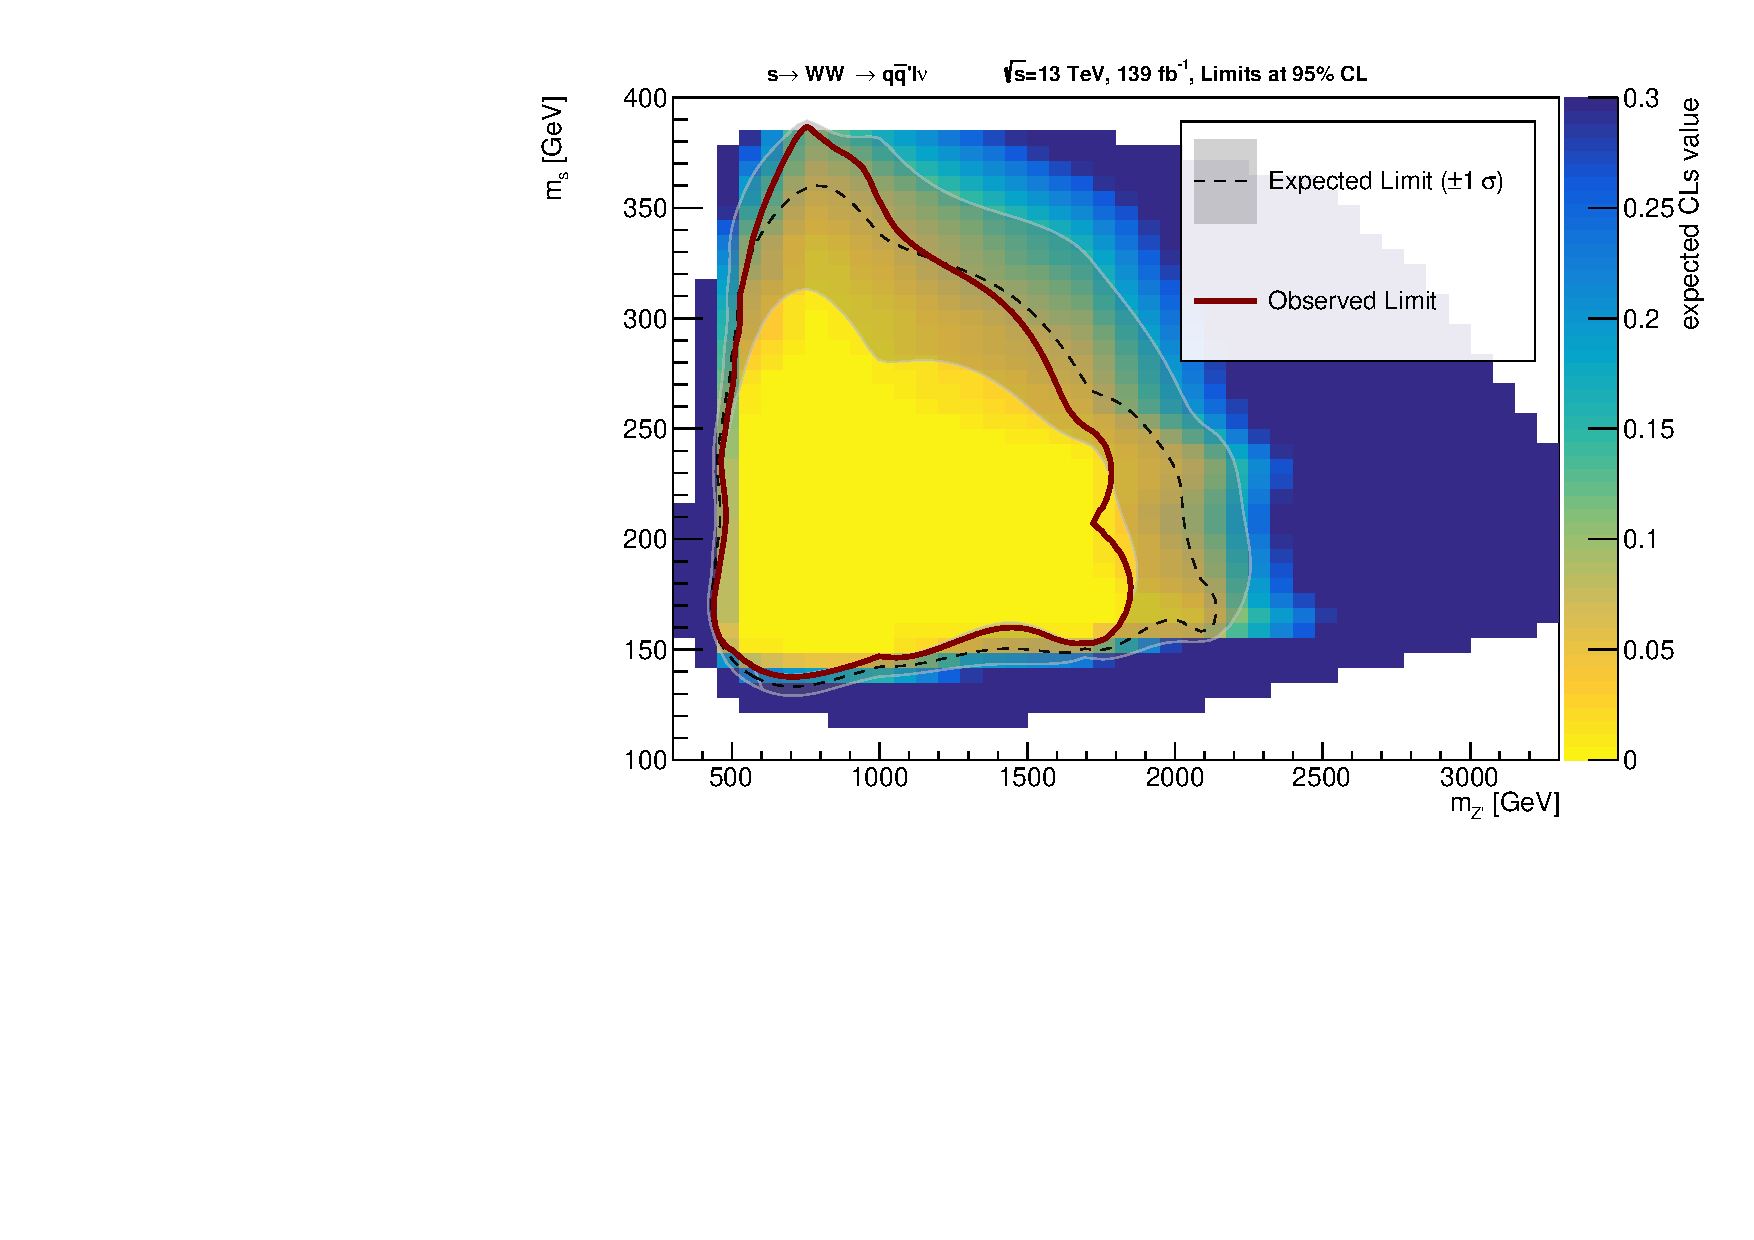
\includegraphics[width=0.8\textwidth]{Figures/8/unblinded_nosig.pdf}
  \caption[]{Expected (grey dashed with \(\pm1\sigma\) uncertainty band) and observed (solid red) range of \ms and \mZp in the DH model excluded by this search. All \ms and \mZp contained within the solid red line are excluded by the search for the choice of \(\mchi=200~\GeV\), \(\sin\theta=0.01\), \(\gchi=1.0\) and \(g_q=0.25\).}
  \label{fig:limits}
\end{figure}

Figure \ref{fig:limits_comparison} summarizes the excluded range of \ms and \mZp in the DH model - for the fixed choices of the DM mass, DH mixing angle and couplings presented at the beginning of this section - by this and all other searches presented in Section \ref{sec:dh_searches} that place constraints on the model by targeting various decay modes of the DH boson \(s\). This search (blue) extends the excluded range for on-shell \(WW\) decays (\(\ms>160~\GeV\)). By additionally probing off-shell \(WW\) decays in the range \(\ms<160\), this search largely closes the pre-existing gap in coverage (\(150~\GeV<\ms<160~\GeV\)) between searches in the \(s\rightarrow WW\) and \(s\rightarrow bb\) DH decay channels.

\begin{figure}[h]
  \centering
  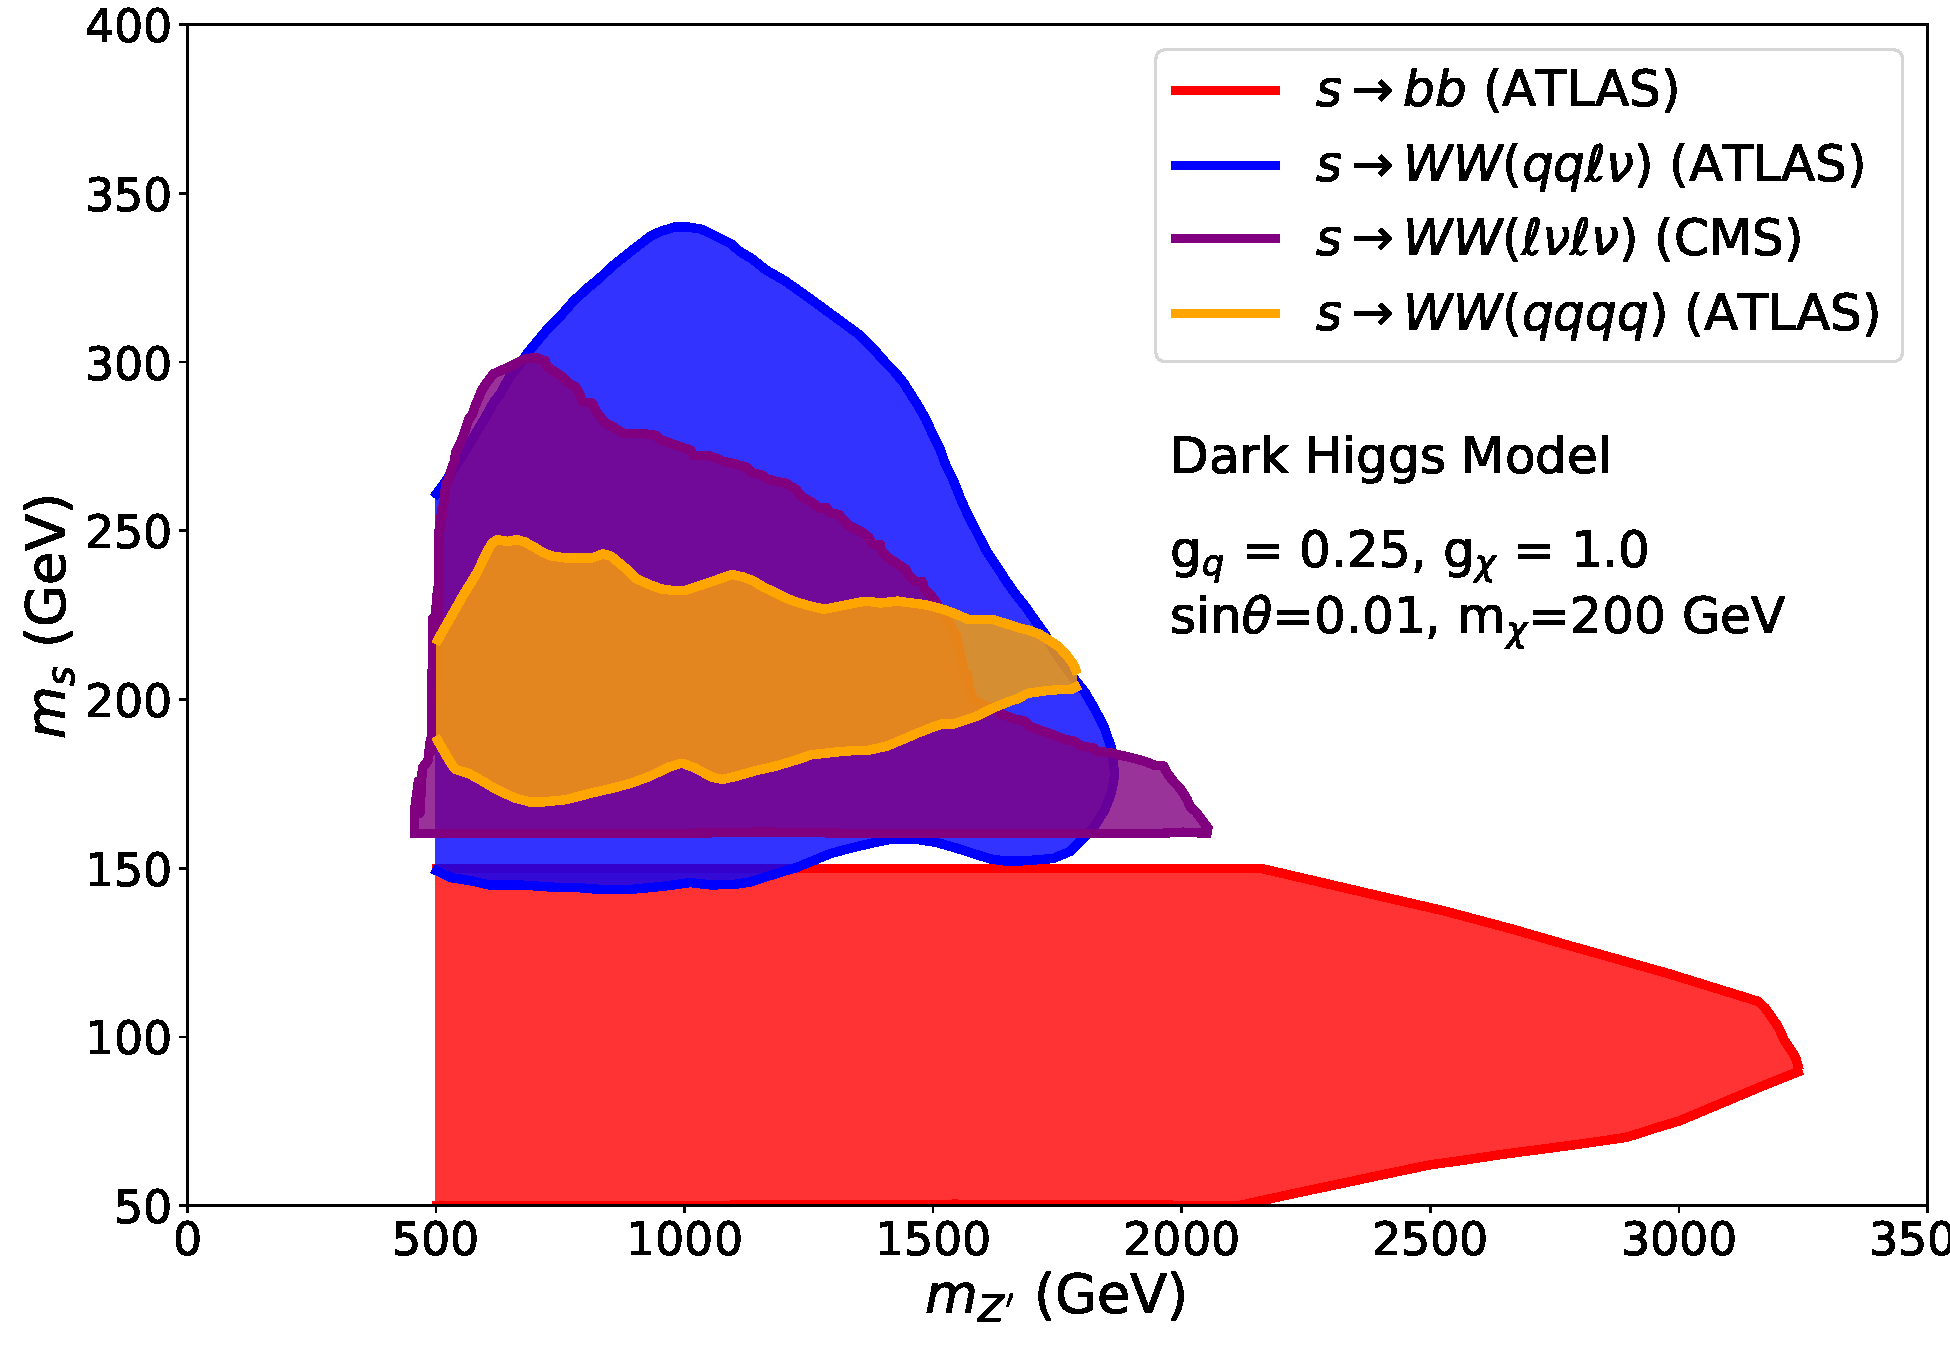
\includegraphics[width=0.8\textwidth]{Figures/8/combined_contour.pdf}
  \caption[]{Summary of \ms and \mZp parameters in the DH model excluded by all searches for the model by ATLAS and CMS. All values of \ms and \mZp contained within a coloured area are excluded. The range excluded by the search presented in this thesis is shown in blue.}
  \label{fig:limits_comparison}
\end{figure}


\subsection{Dependence of Sensitivity on Signal Strength}

Neglecting slight changes to the width of the \Zprime mediator, the production rate of the DH model would be expected to scale in proportion to \(g_q^2\) and \(\gchi^2\) \cite{griffiths_2008} if the values of the \(g_q\) and \(\gchi\) coupling strength parameters, respectively, are varied, since both correspond to a single annihilation (\(g_q\)) or decay (\gchi) vertex in the model (see Figure \ref{fig:Feynman_DH}). As noted in Section \ref{sec:dh_model_free_parameters}, upper bounds are placed on the coupling strength \(g_q\) between the \Zprime mediator and quarks in the DH model by dijet searches, which range from approximately 0.04 to 0.2 depending on the value of \mZp, and on the methods the assumptions involved in placing the constraints. However, the actual value of \gchi in the model is unknown, and is not currently constrained by dijet or other searches. 

Given the dependence of the production rate on the choices of \(g_q\) and \(\gchi\), a test was done following recommendations in Ref. \cite{boveia2016recommendations} to evaluate the impact of reducing the production rate of the DH process on the sensitivity of the search. Implicit in this test is a simplifying assumption that the modified values of \(g_q\) and \(\gchi\) associated with reducing \(\mu\) will result in the same distributions of kinematic variables as the benchmark choices, such that the predicted yields of the signal model in all regions and bins of the search scale linearly with \(\mu\). Figure \ref{fig:limits_vary_mu_sig} compares the range of \ms and \mZp excluded by the search with the value of a ``signal strength" parameter \(\mu\), which coherently scales the production rate of the DH signal process at all \ms and \mZp considered in the search. The search is able to exclude phase space in the \ms vs. \mZp plane for \(\mu\) down to 0.4, with the excluded range successively diminished as \(\mu\) is reduced.



%	\startfirstchapter{Conclusion}
\label{chapter:conclusion}

The study presented in this thesis is part of a worldwide programme to search for dark matter using particle physics detectors, and focusses in particular on dark matter production at the LHC. Given the potential for yet-unconceived mechanisms by which the hypothetical interactions between dark matter and the Standard Model could occur, the search programme at the LHC emphasizes a comprehensive coverage of the possible final states that could result in the detector from dark matter production in the high-energy \(pp\) collisions, with searches guided by and interpreted using simplified models for the dark matter production mechanisms. While there could be many possible dark matter production mechanisms that would predict a signature in the \(\met+WW\) final state studied in this thesis, the construction and interpretation of the search are guided by the Dark Higgs model \cite{Duerr2017}. No statistically significant deviation was found between distributions of ATLAS collision events in the signal regions and Standard Model predictions. The search places exclusion limits on the Dark Higgs model for masses of the Dark Higgs mediator in the approximate range of 150 GeV to 350 GeV. As shown in the summary plot in Figure \ref{fig:limits_comparison}, the parameter space of the Dark Higgs model excluded by this search extends the reach of existing searches for the model performed by the ATLAS and CMS collaborations \cite{monos_had_paper,cms_monos_lep,ATL-PHYS-PUB-2019-032}, which targeted different final states.

The semileptonic \(WW(qq\ell\nu\)) final state studied by this search presented a number of opportunities compared with alternative \(WW\) decay modes to develop targeted data selections and analysis strategies that enhance the sensitivity of the search in this final state. The requirement of a single energetic lepton in the final state allows for a significant reduction of SM background processes relative to the fully hadronic channel, and the \wjets process that dominates the Standard Model background in this semileptonic final state is massively reduced by the application of a lower bound on the transverse mass between the final-state lepton and the \met. In addition, the distinct decay modes of the two \(W\) bosons enable a detailed reconstruction of the hadronically decaying \(W\). This reconstruction is facilitated in the boosted merged regime by a modification to the basic TAR algorithm \cite{TAR_algo} used to reconstruct hadronic activity in the final state within one or more large-radius jets, where the modification additionally disentangles the final-state lepton from the hadronic activity. Targeted selections involving the reconstructed hadronically decaying \(W\) further reduce the background of SM processes in the search. Although the final-state neutrino prevents a full reconstruction of the Dark Higgs boson, the \minms strategy allows for an approximate reconstruction, which provides valuable shape discrimination between the DH signal model and SM background processes in the signal regions.

While the searches that target the \(WW\) final state were optimized to probe the Dark Higgs model, it is important to acknowledge that appreciable constraints on the Dark Higgs model were also obtained in the \(bb\) final state \cite{ATL-PHYS-PUB-2019-032} by re-interpreting an existing dark matter search \cite{ATLAS-CONF-2018-039} that targeted the same final state, but which was optimized to probe a different model. The impressive sensitivity of the re-interpreted search in the \(bb\) final state to the Dark Higgs model highlights the value of ensuring that searches in this \(\met+WW\) final state can also be re-interpreted in the future to constrain any alternative models that may predict a signature in the same final state. This search has been preserved for future re-interpretation using the RECAST framework \cite{Cranmer2011} developed within the ATLAS collaboration. More generally, given the vast multitude of mechanisms by which dark matter could be produced at the LHC, and the tremendous amount of human effort and computing resources involved in developing searches to probe new final states, it will be important moving forward to ensure that all new searches for dark matter can be efficiently re-interpreted to constrain alternative models, thus maximizing the potential impact of each search. 

Despite longstanding evidence from observational astronomy for the abundance of dark matter in the universe, its composition remains one of the open mysteries of modern physics. Each time that a new model is tested or new parameter space is probed, a collective step is taken towards cracking the mystery of what makes up the most abundant form of matter in the universe. 
%	\appendix
%	\startappendix{Kinematic Distributions in Signal and Control Regions}
\label{chapter:appendix_SR_CR_distributions}

This appendix documents comparisons of the distributions of kinematic variables of interest for the search between the signal region (SR) and each control region (CR), considering the merged and resolved categories separately. The aim of these comparisons is to validate that, within each of the merged and resolved categories, the kinematic properties of events in the CRs are sufficiently similar to those in the corresponding SR that the data-driven normalization factors for the \wjets and \ttbar background processes, which are evaluated primarily by comparison with the observed yield of ATLAS collision data in the CRs, can be reasonably applied to scale the predicted yields of these processes in the SR as well. 

\section{Signal region vs. \wjets control region}
\label{app:appendix_SR_CR_distributions_wjets}

\Fig{~\ref{fig:N_1_CRW_merged}} compares distributions of kinematic variables of interest for the analysis between the merged SR and the \wjets CR. \Fig{~\ref{fig:N_1_CRW_resolved}} presents the same comparison between the resolved SR and the \wjets CR.

\begin{figure}[htbp]
  \centering
     \begin{subfigure}{0.45\textwidth}
     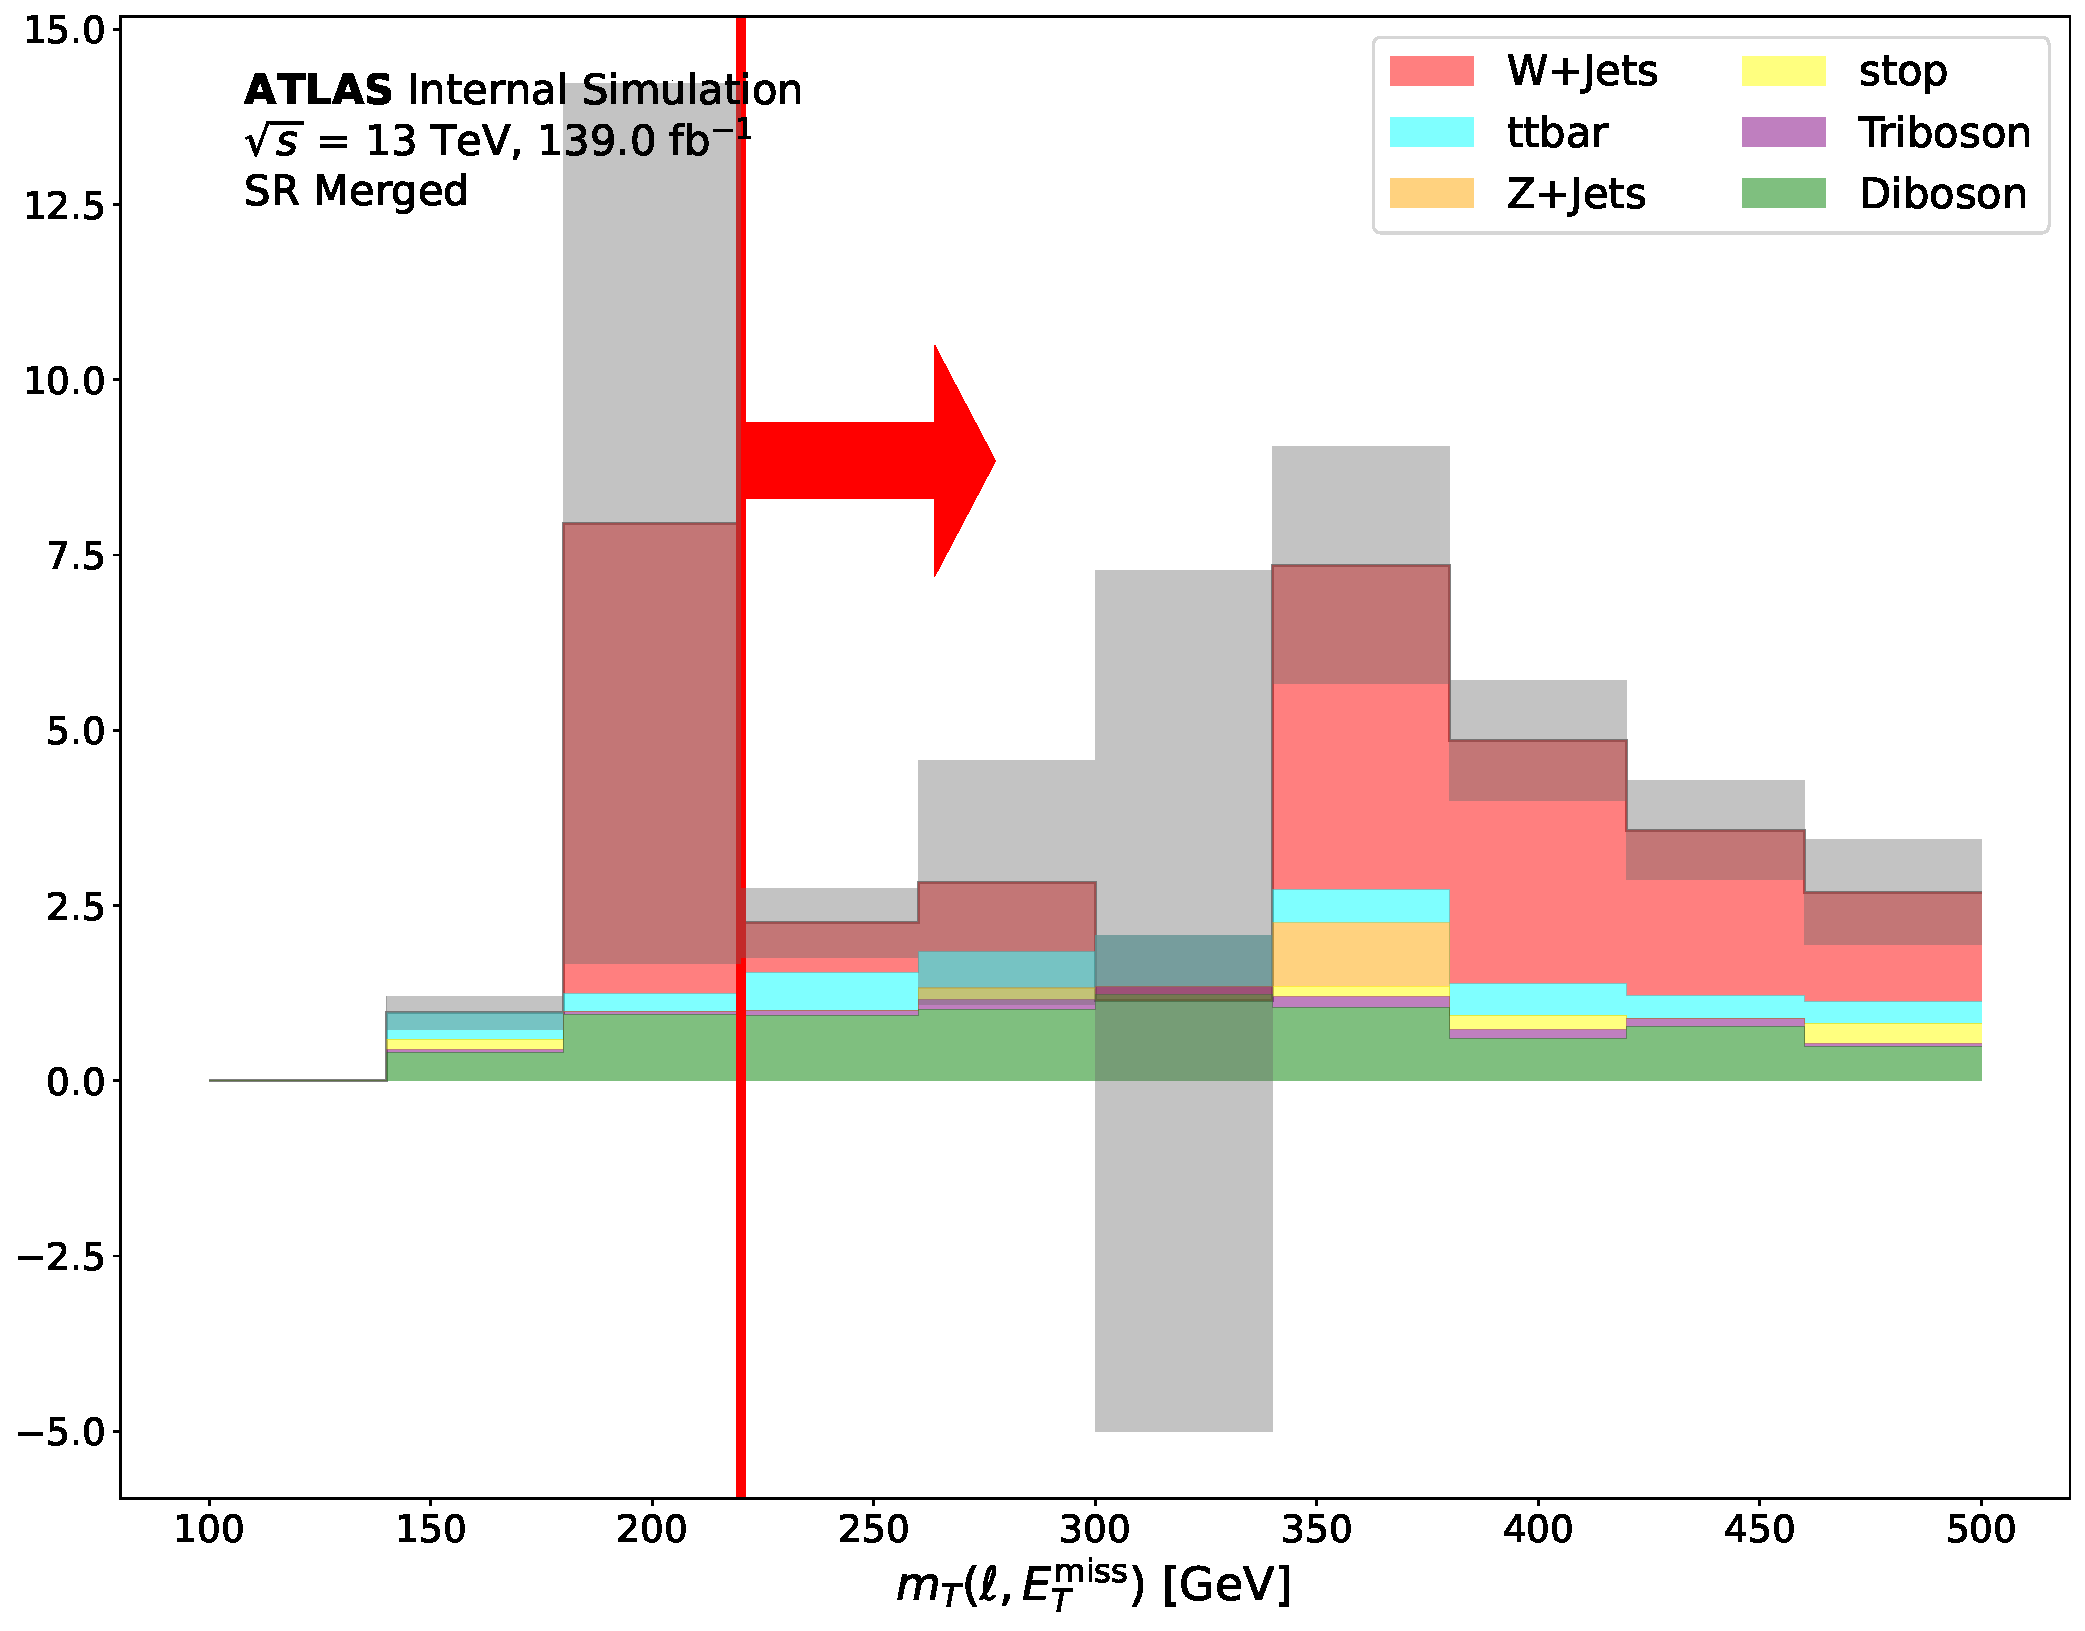
\includegraphics[width = 0.95\textwidth]{Figures/App_SR_CR_distributions/SR1L_Merged/mT_lep_met_N_1.pdf}
    \caption{\mtlepmet (merged SR)}
     \end{subfigure}
    \begin{subfigure}{0.45\textwidth}
     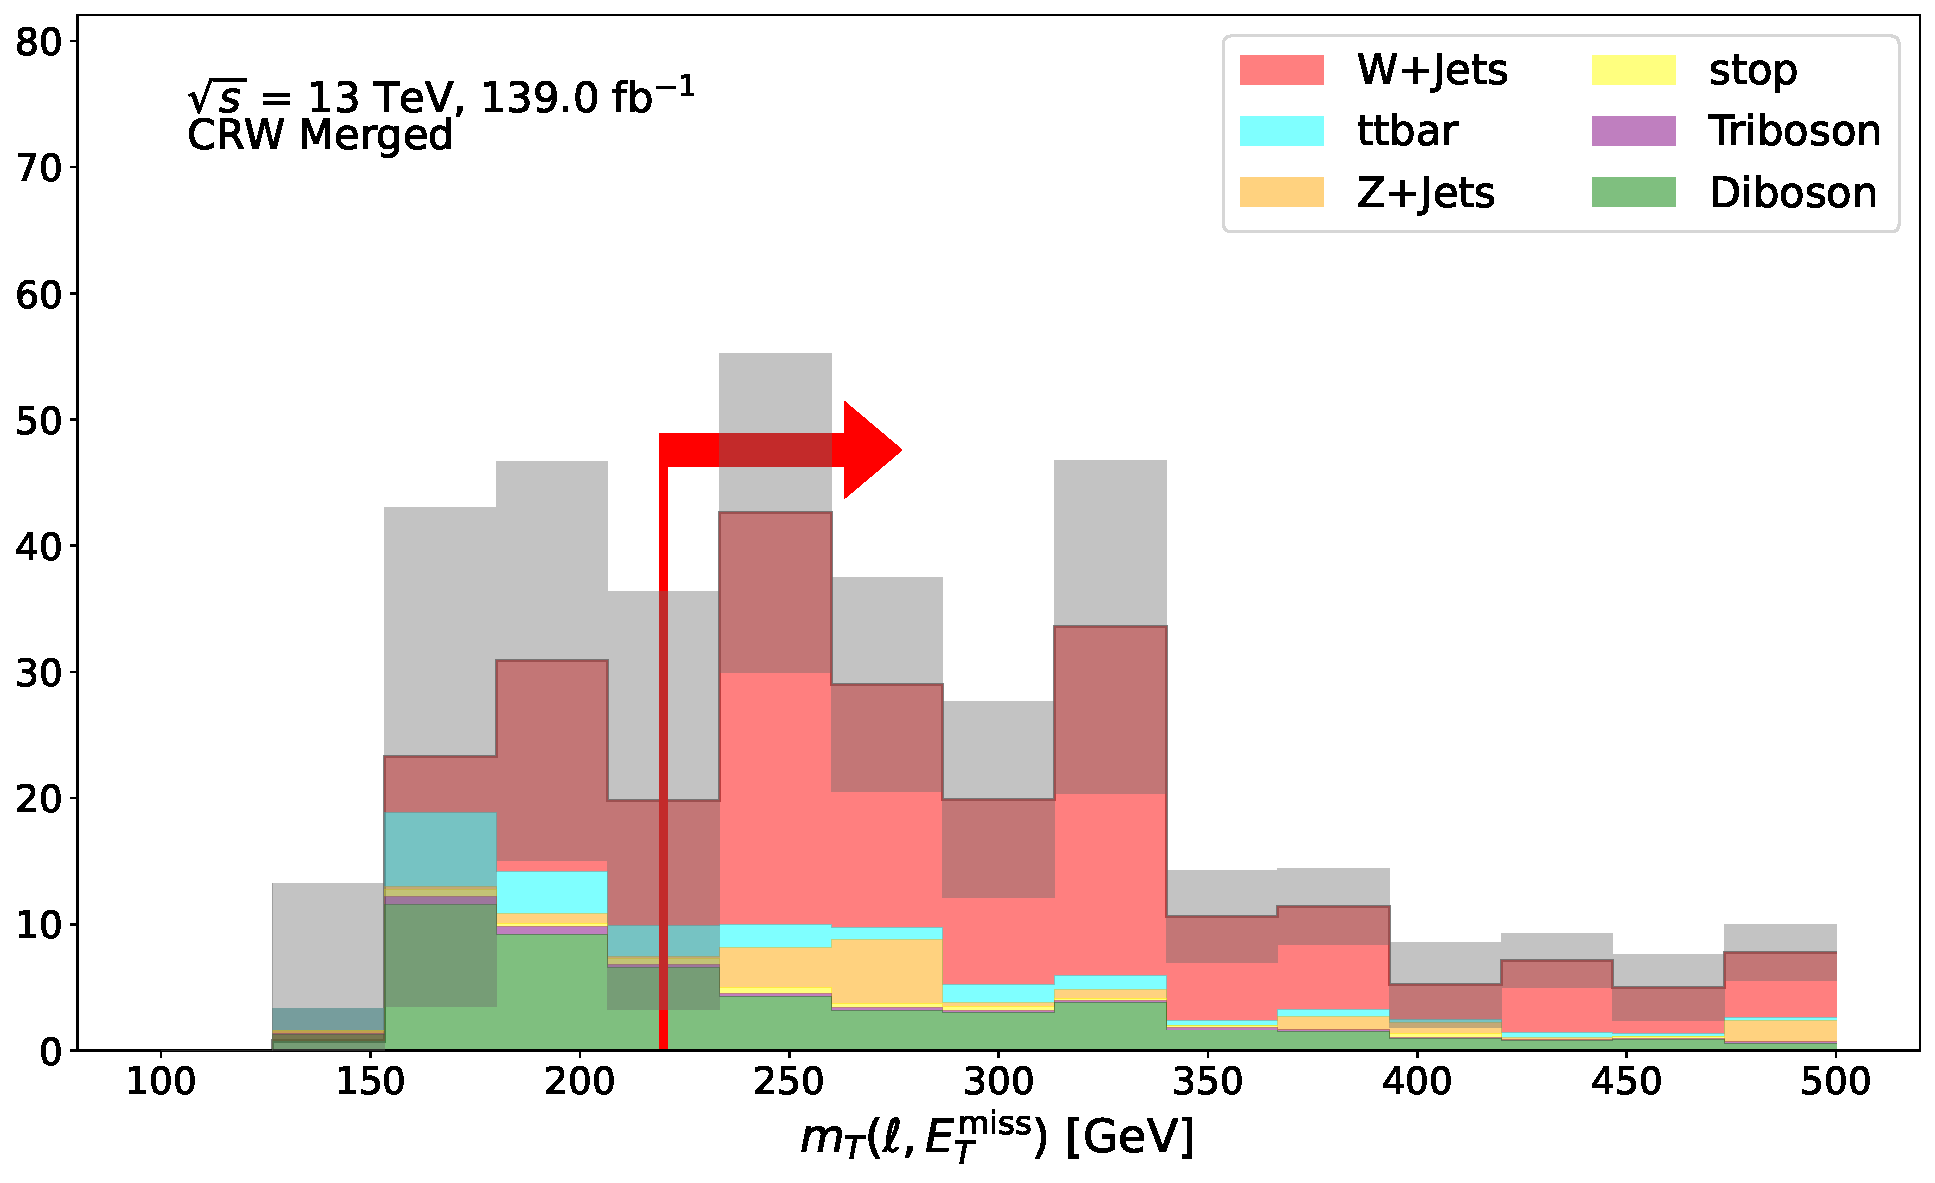
\includegraphics[width = 0.95\textwidth]{Figures/App_SR_CR_distributions/CRW_Merged/mT_lep_met_N_1.pdf}
     \caption{\mtlepmet (merged \wjets CR)}
     \end{subfigure}

      \begin{subfigure}{0.45\textwidth}
     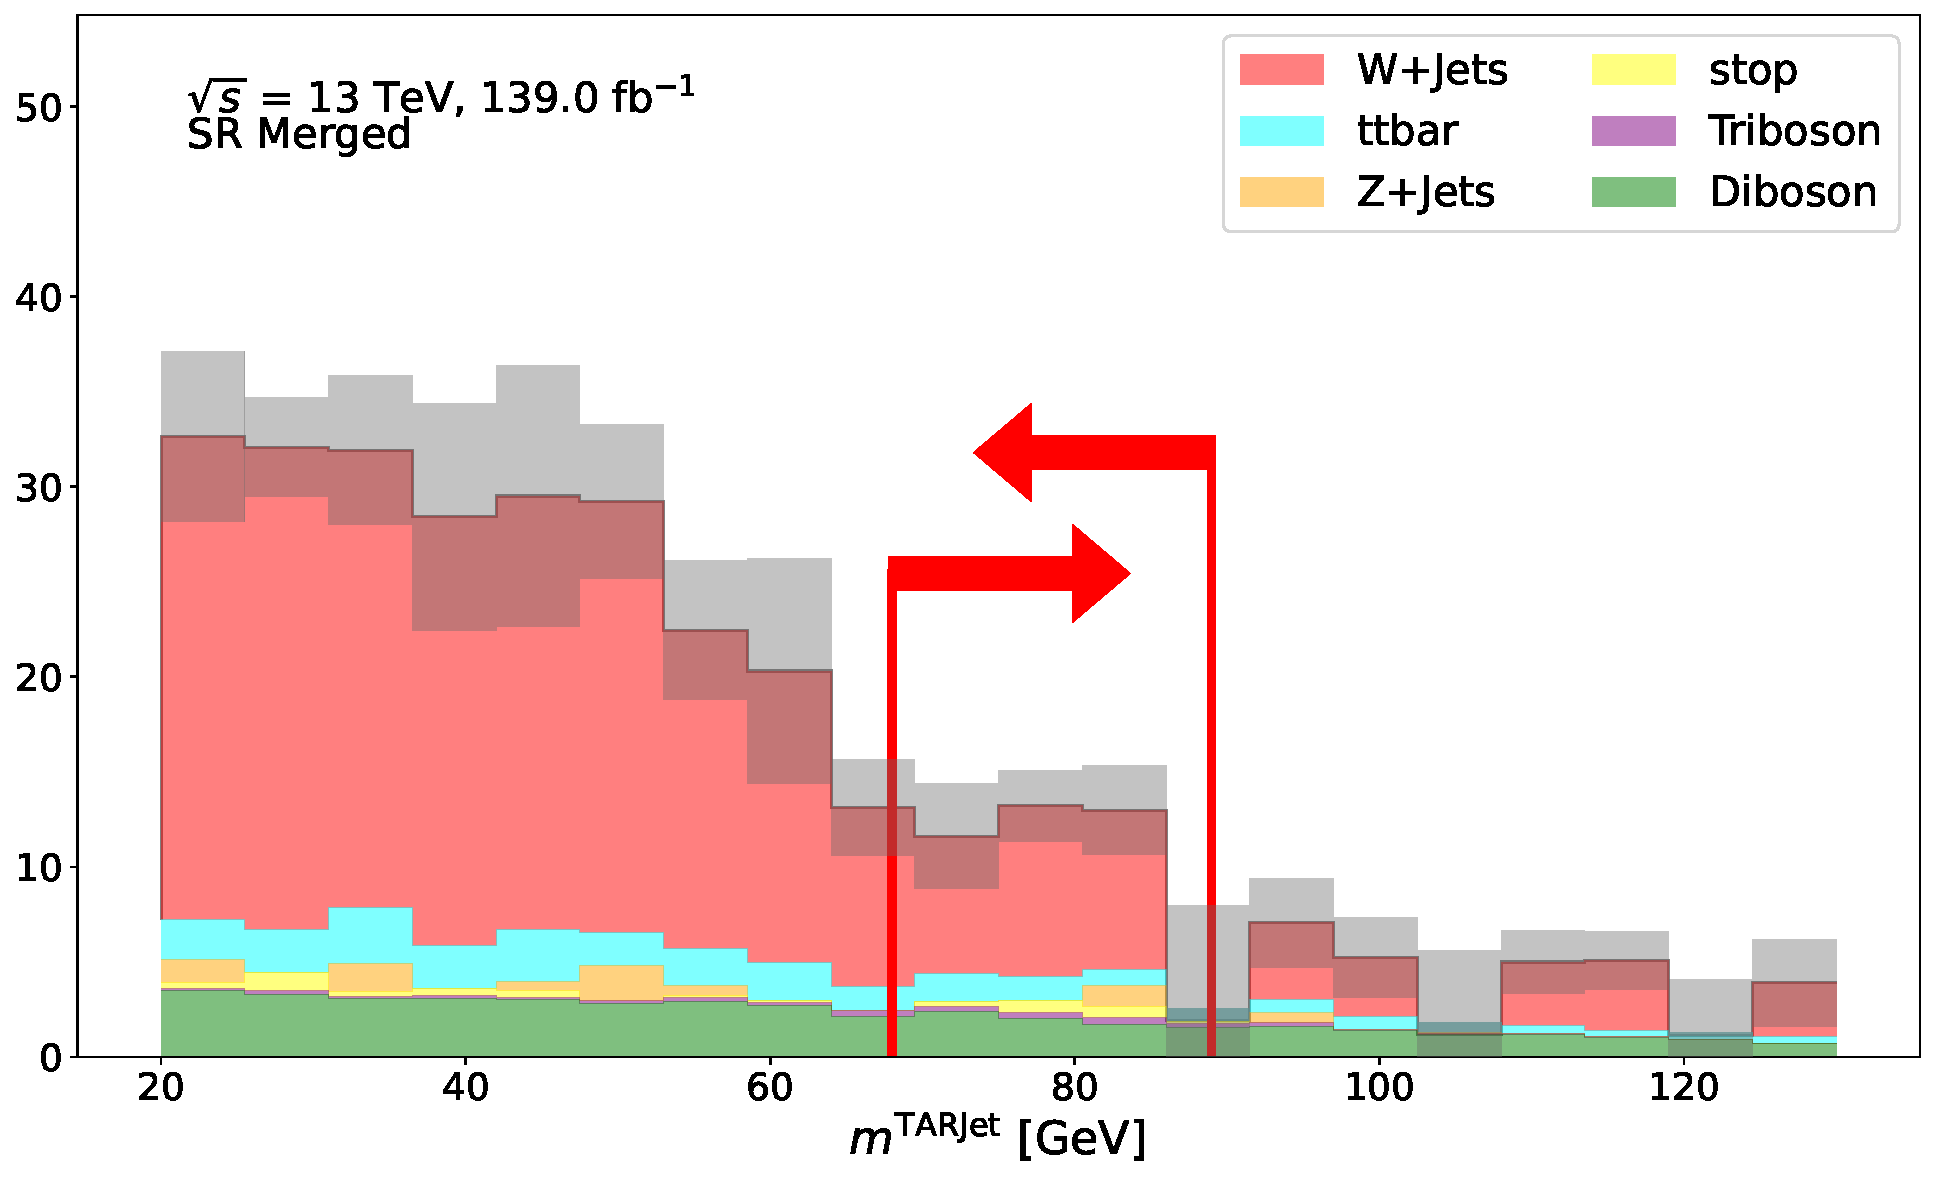
\includegraphics[width = 0.95\textwidth]{Figures/App_SR_CR_distributions/SR1L_Merged/TARJets10_mTAR0_N_1.pdf}
    \caption{\mTAR (merged SR)}
     \end{subfigure}
    \begin{subfigure}{0.45\textwidth}
     \includegraphics[width = 0.95\textwidth]{Figures/App_SR_CR_distributions/CRW_Merged/TARJets10_mTAR0_N_1.pdf}
     \caption{\mTAR (merged \wjets CR)}
     \end{subfigure}

 \begin{subfigure}{0.45\textwidth}
     \includegraphics[width = 0.95\textwidth]{Figures/App_SR_CR_distributions/SR1L_Merged/MetTST_Significance_N_1.pdf}
    \caption{\metsig (merged SR)}
     \end{subfigure}
    \begin{subfigure}{0.45\textwidth}
     \includegraphics[width = 0.95\textwidth]{Figures/App_SR_CR_distributions/CRW_Merged/MetTST_Significance_N_1.pdf}
     \caption{\metsig (merged \wjets CR)}
     \end{subfigure}
     
     \caption[Comparison of N-1 distributions for kinematic variables of interest between the signal region and the \wjets control region in the merged category.]{Comparison of N-1 distributions for kinematic variables of interest between the SR and the \wjets CR in the merged category. Grey bands show statistical uncertainty on the background estimate.}
     \label{fig:N_1_CRW_merged}
  \end{figure}
  
  \captionsetup[figure]{list=no}
  
 \begin{figure}[htbp] \ContinuedFloat
   \begin{subfigure}{0.45\textwidth}
     \includegraphics[width = 0.95\textwidth]{Figures/App_SR_CR_distributions/SR1L_Merged/TARJets10_TAR_D20_N_1.pdf}
    \caption{\DtwoTAR (merged SR)}
     \end{subfigure}
    \begin{subfigure}{0.45\textwidth}
     \includegraphics[width = 0.95\textwidth]{Figures/App_SR_CR_distributions/CRW_Merged/TARJets10_TAR_D20_N_1.pdf}
     \caption{\DtwoTAR (merged \wjets CR)}
     \end{subfigure}

   \begin{subfigure}{0.45\textwidth}
     \includegraphics[width = 0.95\textwidth]{Figures/App_SR_CR_distributions/SR1L_Merged/MetTST_met_N_1.pdf}
    \caption{\met (merged SR)}
    \label{fig:N_1_SR_merged_met}
     \end{subfigure}
    \begin{subfigure}{0.45\textwidth}
     \includegraphics[width = 0.95\textwidth]{Figures/App_SR_CR_distributions/CRW_Merged/MetTST_met_N_1.pdf}
     \caption{\met (merged \wjets CR)}
     \label{fig:N_1_CRW_merged_met}
     \end{subfigure}
     \caption{Comparison of N-1 distributions for kinematic variables of interest between the SR and the \wjets CR in the merged category (continued).}
  \end{figure}
  
  \captionsetup[figure]{list=no}

  \begin{figure}[htbp]
  \centering
     \begin{subfigure}{0.45\textwidth}
     \includegraphics[width = 0.95\textwidth]{Figures/App_SR_CR_distributions/SR1L_Resolved/mT_lep_met_N_1.pdf}
    \caption{\mtlepmet (resolved SR)}
     \end{subfigure}
    \begin{subfigure}{0.45\textwidth}
     \includegraphics[width = 0.95\textwidth]{Figures/App_SR_CR_distributions/CRW_Resolved/mT_lep_met_N_1.pdf}
     \caption{\mtlepmet (resolved \wjets CR)}
     \end{subfigure}

  \begin{subfigure}{0.45\textwidth}
     \includegraphics[width = 0.95\textwidth]{Figures/App_SR_CR_distributions/SR1L_Resolved/WCand_m_N_1.pdf}
    \caption{\Wcandm (resolved SR)}
     \end{subfigure}
    \begin{subfigure}{0.45\textwidth}
     \includegraphics[width = 0.95\textwidth]{Figures/App_SR_CR_distributions/CRW_Resolved/WCand_m_N_1.pdf}
     \caption{\Wcandm (resolved \wjets CR)}
     \end{subfigure}

  \begin{subfigure}{0.45\textwidth}
     \includegraphics[width = 0.95\textwidth]{Figures/App_SR_CR_distributions/SR1L_Resolved/MetTST_Significance_N_1.pdf}
    \caption{\metsig (resolved SR)}
     \end{subfigure}
    \begin{subfigure}{0.45\textwidth}
     \includegraphics[width = 0.95\textwidth]{Figures/App_SR_CR_distributions/CRW_Resolved/MetTST_Significance_N_1.pdf}
     \caption{\metsig (resolved \wjets CR)}
     \end{subfigure}
      \caption[Comparison of N-1 distributions for kinematic variables of interest between the signal region and the \wjets control region in the resolved category.]{Comparison of N-1 distributions for kinematic variables of interest between the SR and the \wjets CR in the resolved category. Grey bands show statistical uncertainty on the background estimate.}
     \label{fig:N_1_CRW_resolved}    
     \end{figure}
     
     \captionsetup[figure]{list=no}
     
     \begin{figure}[htbp] \ContinuedFloat
    \begin{subfigure}{0.45\textwidth}
     \includegraphics[width = 0.95\textwidth]{Figures/App_SR_CR_distributions/SR1L_Resolved/WCand_pt_N_1.pdf}
    \caption{\Wcandpt (resolved SR)}
     \end{subfigure}
    \begin{subfigure}{0.45\textwidth}
     \includegraphics[width = 0.95\textwidth]{Figures/App_SR_CR_distributions/CRW_Resolved/WCand_pt_N_1.pdf}
     \caption{\Wcandpt (resolved \wjets CR)}
     \end{subfigure}   
    \begin{subfigure}{0.45\textwidth}
     \includegraphics[width = 0.95\textwidth]{Figures/App_SR_CR_distributions/SR1L_Resolved/MetTST_met_N_1.pdf}
    \caption{\met (resolved SR)}
     \end{subfigure}
    \begin{subfigure}{0.45\textwidth}
     \includegraphics[width = 0.95\textwidth]{Figures/App_SR_CR_distributions/CRW_Resolved/MetTST_met_N_1.pdf}
     \caption{\met (resolved \wjets CR)}
     \end{subfigure}
     \caption{Comparison of N-1 distributions for kinematic variables of interest between the SR and the \wjets CR in the resolved category (continued).}
  \end{figure}
  
  \captionsetup[figure]{list=yes}


\section{Signal region vs. \ttbar control region}
\label{app:appendix_SR_CR_distributions_ttbar}

\Fig{~\ref{fig:N_1_CRTT_merged}} compares distributions of kinematic variables of interest for the analysis between the merged SR and the \ttbar CR. \Fig{~\ref{fig:N_1_CRTT_resolved}} presents the same comparisons between the resolved SR and the \ttbar CR.

\begin{figure}[htbp]
  \centering
     \begin{subfigure}{0.45\textwidth}
     \includegraphics[width = 0.95\textwidth]{Figures/App_SR_CR_distributions/SR1L_Merged/mT_lep_met_N_1.pdf}
    \caption{\mtlepmet (merged SR)}
     \end{subfigure}
    \begin{subfigure}{0.45\textwidth}
     \includegraphics[width = 0.95\textwidth]{Figures/App_SR_CR_distributions/CRTT_Merged/mT_lep_met_N_1.pdf}
     \caption{\mtlepmet (merged \ttbar CR)}
     \end{subfigure}

      \begin{subfigure}{0.45\textwidth}
     \includegraphics[width = 0.95\textwidth]{Figures/App_SR_CR_distributions/SR1L_Merged/TARJets10_mTAR0_N_1.pdf}
    \caption{\mTAR (merged SR)}
     \end{subfigure}
    \begin{subfigure}{0.45\textwidth}
     \includegraphics[width = 0.95\textwidth]{Figures/App_SR_CR_distributions/CRTT_Merged/TARJets10_mTAR0_N_1.pdf}
     \caption{\mTAR (merged \ttbar CR)}
     \end{subfigure}

 \begin{subfigure}{0.45\textwidth}
     \includegraphics[width = 0.95\textwidth]{Figures/App_SR_CR_distributions/SR1L_Merged/MetTST_Significance_N_1.pdf}
    \caption{\metsig (merged SR)}
     \end{subfigure}
    \begin{subfigure}{0.45\textwidth}
     \includegraphics[width = 0.95\textwidth]{Figures/App_SR_CR_distributions/CRTT_Merged/MetTST_Significance_N_1.pdf}
     \caption{\metsig (merged \ttbar CR)}
     \end{subfigure}
      \caption[Comparison of N-1 distributions for kinematic variables of interest between the signal region and the ttbar control region in the merged category.]{Comparison of N-1 distributions for kinematic variables of interest between the SR and the \ttbar CR in the merged category. Grey bands show statistical uncertainty on the background estimate.}
      \label{fig:N_1_CRTT_merged}
       \end{figure}
       
       \captionsetup[figure]{list=no}
       
    \begin{figure}[htbp]\ContinuedFloat
  \begin{subfigure}{0.45\textwidth}
     \includegraphics[width = 0.95\textwidth]{Figures/App_SR_CR_distributions/SR1L_Merged/dR_lep_TARJets10_N_1.pdf}
    \caption{\drTARl (merged SR)}
     \end{subfigure}
    \begin{subfigure}{0.45\textwidth}
     \includegraphics[width = 0.95\textwidth]{Figures/App_SR_CR_distributions/CRTT_Merged/dR_lep_TARJets10_N_1.pdf}
     \caption{\drTARl (merged \ttbar CR)}
     \end{subfigure}

   \begin{subfigure}{0.45\textwidth}
     \includegraphics[width = 0.95\textwidth]{Figures/App_SR_CR_distributions/SR1L_Merged/TARJets10_TAR_D20_N_1.pdf}
    \caption{\DtwoTAR (merged SR)}
     \end{subfigure}
    \begin{subfigure}{0.45\textwidth}
     \includegraphics[width = 0.95\textwidth]{Figures/App_SR_CR_distributions/CRTT_Merged/TARJets10_TAR_D20_N_1.pdf}
     \caption{\DtwoTAR (merged \ttbar CR)}
     \end{subfigure}

   \begin{subfigure}{0.45\textwidth}
     \includegraphics[width = 0.95\textwidth]{Figures/App_SR_CR_distributions/SR1L_Merged/MetTST_met_N_1.pdf}
    \caption{\met (merged SR)}
     \end{subfigure}
    \begin{subfigure}{0.45\textwidth}
     \includegraphics[width = 0.95\textwidth]{Figures/App_SR_CR_distributions/CRTT_Merged/MetTST_met_N_1.pdf}
     \caption{\met (merged \ttbar CR)}
     \end{subfigure}
     \caption{Comparison of N-1 distributions for kinematic variables of interest between the SR and the \ttbar CR in the merged category (continued).}
  \end{figure}

\captionsetup[figure]{list=yes}

  \begin{figure}[htbp]
  \centering

     \begin{subfigure}{0.45\textwidth}
     \includegraphics[width = 0.95\textwidth]{Figures/App_SR_CR_distributions/SR1L_Resolved/mT_lep_met_N_1.pdf}
    \caption{\mtlepmet (resolved SR)}
     \end{subfigure}
    \begin{subfigure}{0.45\textwidth}
     \includegraphics[width = 0.95\textwidth]{Figures/App_SR_CR_distributions/CRTT_Resolved/mT_lep_met_N_1.pdf}
     \caption{\mtlepmet (resolved \ttbar CR)}
     \end{subfigure}

  \begin{subfigure}{0.45\textwidth}
     \includegraphics[width = 0.95\textwidth]{Figures/App_SR_CR_distributions/SR1L_Resolved/WCand_m_N_1.pdf}
    \caption{\Wcandm (resolved SR)}
     \end{subfigure}
    \begin{subfigure}{0.45\textwidth}
     \includegraphics[width = 0.95\textwidth]{Figures/App_SR_CR_distributions/CRTT_Resolved/WCand_m_N_1.pdf}
     \caption{\Wcandm (resolved \ttbar CR)}
     \end{subfigure}

  \begin{subfigure}{0.45\textwidth}
     \includegraphics[width = 0.95\textwidth]{Figures/App_SR_CR_distributions/SR1L_Resolved/MetTST_Significance_N_1.pdf}
    \caption{\metsig (resolved SR)}
     \end{subfigure}
    \begin{subfigure}{0.45\textwidth}
     \includegraphics[width = 0.95\textwidth]{Figures/App_SR_CR_distributions/CRTT_Resolved/MetTST_Significance_N_1.pdf}
     \caption{\metsig (resolved \ttbar CR)}
     \end{subfigure}
     \caption[Comparison of N-1 distributions for kinematic variables of interest between the signal region and the \ttbar control region in the resolved category.]{Comparison of N-1 distributions for kinematic variables of interest between the SR and the \ttbar CR in the merged category. Grey bands show statistical uncertainty on the background estimate.}
     \label{fig:N_1_CRTT_resolved}
     \end{figure}
     
     \captionsetup[figure]{list=no}

    \begin{figure}[htbp]\ContinuedFloat
   \begin{subfigure}{0.45\textwidth}
     \includegraphics[width = 0.95\textwidth]{Figures/App_SR_CR_distributions/SR1L_Resolved/dRWl_N_1.pdf}
    \caption{\drWl (resolved SR)}
     \end{subfigure}
    \begin{subfigure}{0.45\textwidth}
     \includegraphics[width = 0.95\textwidth]{Figures/App_SR_CR_distributions/CRTT_Resolved/dRWl_N_1.pdf}
     \caption{\drWl (resolved \ttbar CR)}
     \end{subfigure}

    \begin{subfigure}{0.45\textwidth}
     \includegraphics[width = 0.95\textwidth]{Figures/App_SR_CR_distributions/SR1L_Resolved/WCand_pt_N_1.pdf}
    \caption{\Wcandpt (resolved SR)}
     \end{subfigure}
    \begin{subfigure}{0.45\textwidth}
     \includegraphics[width = 0.95\textwidth]{Figures/App_SR_CR_distributions/CRTT_Resolved/WCand_pt_N_1.pdf}
     \caption{\Wcandpt (resolved \ttbar CR)}
     \end{subfigure}
     
    \begin{subfigure}{0.45\textwidth}
     \includegraphics[width = 0.95\textwidth]{Figures/App_SR_CR_distributions/SR1L_Resolved/MetTST_met_N_1.pdf}
    \caption{\met (resolved SR)}
     \end{subfigure}
    \begin{subfigure}{0.45\textwidth}
     \includegraphics[width = 0.95\textwidth]{Figures/App_SR_CR_distributions/CRTT_Resolved/MetTST_met_N_1.pdf}
     \caption{\met (resolved \ttbar CR)}
     \end{subfigure}

     \caption{Comparison of N-1 distributions for kinematic variables of interest between the SR and the \ttbar CR in the merged category (continued)}
  \end{figure}
  
  \captionsetup[figure]{list=yes}


%	\startappendix{Nuisance Parameter Descriptions for Systematics}
\label{chapter:appendix_systematics_descriptions}

Tables \ref{tab:exp_syst_naming} and \ref{tab:theo_syst_naming} provide qualitative descriptions of the NPs used to parametrize systematic uncertainties in the likelihood function presented in Section \ref{sec:likelihood}. Details of the systematic uncertainty sources can be found in Chapter \ref{chapter:systematics}.

{
\scriptsize
\begin{longtable}{p{7cm} p{8cm}}
\caption[Qualitative description of nuisance parameters associated with sources of experimental systematic uncertainty considered in the search.]{Qualitative description of NPs associated with sources of experimental systematic uncertainty considered in the search.} \label{tab:exp_syst_naming} \\
\toprule
\textbf{Nuisance Parameter} & \textbf{Short Description}              \\ 
\midrule 
\midrule 
\multicolumn{2}{c}{\textbf{Event}} \\ \midrule
\(\alpha\)\_lumiSys  & uncertainty on the total integrated luminosity   \\ \midrule
\(\alpha\)\_PRW\_DATASF  & pileup reweighting uncertainty   \\ \midrule

\multicolumn{2}{c}{\textbf{Electrons}}  \\ \midrule
\(\alpha\)\_EL\_EFF\_Reco\_TOTAL\_1NPCOR\_PLUS\_UNCOR    & reconstruction efficiency uncertainty        \\
\(\alpha\)\_EL\_EFF\_ID\_TOTAL\_1NPCOR\_PLUS\_UNCOR    & ID efficiency uncertainty     \\
\(\alpha\)\_EL\_EFF\_Iso\_TOTAL\_1NPCOR\_PLUS\_UNCOR    & isolation efficiency uncertainty     \\
\(\alpha\)\_EG\_SCALE\_ALL & energy scale uncertainty  \\
\(\alpha\)\_EG\_RESOLUTION\_ALL & energy resolution uncertainty  \\ \midrule

\multicolumn{2}{c}{\textbf{Muons}}  \\ \midrule
\(\alpha\)\_MUON\_EFF\_TrigSystUncertainty        & \multirow{2}{*}{trigger efficiency uncertainties}    \\
\(\alpha\)\_MUON\_EFF\_TrigStatUncertainty        &    \\
\(\alpha\)\_MUON\_EFF\_RECO\_STAT        & \multirow{ 2}{*}{reconstruction and ID efficiency uncertainty for \(\pt > 15~\GeV\)}      \\
\(\alpha\)\_MUON\_EFF\_RECO\_SYS      \\
\(\alpha\)\_MUON\_EFF\_RECO\_STAT\_LOWPT        & \multirow{ 2}{*}{reconstruction and ID efficiency uncertainty for \(\pt < 15~\GeV\)}     \\
\(\alpha\)\_MUON\_EFF\_RECO\_SYS\_LOWPT        \\
\(\alpha\)\_MUON\_EFF\_ISO\_STAT        & \multirow{ 2}{*}{isolation efficiency uncertainty}        \\
\(\alpha\)\_MUON\_EFF\_ISO\_SYS            \\
\(\alpha\)\_MUON\_EFF\_TTVA\_STAT       & \multirow{ 2}{*}{track-to-vertex association efficiency uncertainty}      \\
\(\alpha\)\_MUON\_EFF\_TTVA\_SYS         \\

\(\alpha\)\_MUON\_SCALE            & energy scale uncertainty                \\
\(\alpha\)\_MUON\_ID               & energy resolution uncertainty from inner detector    \\
\(\alpha\)\_MUON\_MS               & energy resolution uncertainty from muon system     \\
\(\alpha\)\_MUON\_SAGITTA\_RESBIAS & uncertainty in the momentum scale  \\
\(\alpha\)\_MUON\_SAGITTA\_RHO     & uncertainty in the momentum scale   \\

% \midrule
% \multicolumn{2}{c}{\textbf{Taus}}  \\ \midrule
% TAUS\_TRUEHADTAU\_SME\_TES\_DETECTOR  & energy scale uncertainty (detector effects)    \\
% TAUS\_TRUEHADTAU\_SME\_TES\_INSITUFIT & energy scale uncertainty (in-situ correction)   \\
% TAUS\_TRUEHADTAU\_SME\_TES\_INSITUEXP & energy scale uncertainty (in-situ correction)   \\
% TAUS\_TRUEHADTAU\_SME\_TES\_MODEL     & tau-related uncertainty (MC modeling)        \\

\midrule
\multicolumn{2}{c}{\textbf{\akt \(R=0.4\) jets}}  \\
\midrule
\(\alpha\)\_JET\_EffectiveNP\_Detector   & JES uncertainty: detector effects (2 components)       \\
\(\alpha\)\_JET\_EffectiveNP\_Mixed      & JES uncertainty: mixed effects (3 components)          \\
\(\alpha\)\_JET\_EffectiveNP\_Modelling  & JES uncertainty: modelling effects (5 components)        \\
\(\alpha\)\_JET\_EffectiveNP\_Statistical  & JES uncertainty: statistical uncertainty (6 components)         \\
\(\alpha\)\_JET\_EtaIntercalibration\_Modelling            & \multirow{6}{*}{uncertainties in scale calibration of forward / central jets}  \\
\(\alpha\)\_JET\_EtaIntercalibration\_NonClosure\_2018data &    \\
\(\alpha\)\_JET\_EtaIntercalibration\_NonClosure\_highE    &     \\
\(\alpha\)\_JET\_EtaIntercalibration\_NonClosure\_negEta  &    \\
\(\alpha\)\_JET\_EtaIntercalibration\_NonClosure\_posEta  &    \\
\(\alpha\)\_JET\_EtaIntercalibration\_TotalStat &  \\
\(\alpha\)\_JET\_BJES\_Response      & \multirow{3}{*}{flavour-related uncertainties}  \\
\(\alpha\)\_JET\_Flavor\_Composition &   \\
\(\alpha\)\_JET\_Flavor\_Response    &    \\
\(\alpha\)\_JET\_JER\_EffectiveNP    & jet energy resolution uncertainty (12 components)  \\
\(\alpha\)\_JET\_JER\_DataVsMC\_MC16 & jet energy resolution uncertainty (data vs. MC)  \\
\(\alpha\)\_JET\_JvtEfficiency       & jet-vertex-tagger efficiency uncertainty   \\
\(\alpha\)\_JET\_Pileup\_OffsetMu    & \multirow{4}{*}{Pileup uncertainties}  \\
\(\alpha\)\_JET\_Pileup\_OffsetNPV   &    \\
\(\alpha\)\_JET\_Pileup\_PtTerm &  \\
\(\alpha\)\_JET\_Pileup\_RhoTopology &   \\
\(\alpha\)\_JET\_PunchThrough\_MC16 & punch through uncertainty  \\
\midrule

\multicolumn{2}{c}{\textbf{Tagging efficiency (using \akt \(R=0.4\) jets)}} \\
\midrule
\(\alpha\)\_FT\_EFF\_EIGEN\_B & \(b\)-tagging efficiency uncs (medium eigenvector decomp. of flavour tagging uncs)  \\
\(\alpha\)\_FT\_EFF\_EIGEN\_C & \multirow{2}{*}{3 components for \(b\)-jets, 4 for \(c\)-jets and 5 for light jets}    \\
\(\alpha\)\_FT\_EFF\_EIGEN\_L  \\
\(\alpha\)\_FT\_EFF\_EIGEN\_extrapolation &  \(b\)-tagging efficiency uncertainty on the extrapolation on high \pt-jets \\
\(\alpha\)\_FT\_EFF\_EIGEN\_extrapolation\_from\_charm & \(b\)-tagging efficiency uncertainty on \(\tau\)-jets \\ 
\midrule

\multicolumn{2}{c}{\textbf{Rscan \(R=0.2\) jets used for TAR jet construction }}  \\
\midrule
\(\alpha\)\_JET\_R02\_EffectiveNP\_Detector   & JES uncertainty: detector effects (2 components)        \\
\(\alpha\)\_JET\_R02\_EffectiveNP\_Mixed      & JES uncertainty: mixed effects (3 components)            \\
\(\alpha\)\_JET\_R02\_EffectiveNP\_Modelling  & JES uncertainty: modelling effects (5 components)         \\
\(\alpha\)\_JET\_R02\_EffectiveNP\_Statistical  & JES uncertainty: statistical uncertainty (6 components)         \\
\(\alpha\)\_JET\_R02\_EtaIntercalibration\_Modelling            & \multirow{5}{*}{uncertainties in scale calibration of forward / central jets}  \\
\(\alpha\)\_JET\_R02\_EtaIntercalibration\_NonClosure\_highE    &  \\
\(\alpha\)\_JET\_R02\_EtaIntercalibration\_NonClosure\_negEta  &   \\
\(\alpha\)\_JET\_R02\_EtaIntercalibration\_NonClosure\_posEta  &  \\
\(\alpha\)\_JET\_R02\_EtaIntercalibration\_TotalStat &  \\
\(\alpha\)\_JET\_R02\_BJES\_Response      & \multirow{3}{*}{flavour-related uncertainty}  \\
\(\alpha\)\_JET\_R02\_Flavor\_Composition &   \\
\(\alpha\)\_JET\_R02\_Flavor\_Response    &  \\
\(\alpha\)\_JET\_R02\_JER\_EffectiveNP    & jet energy resolution uncertainty (17 components)  \\
\(\alpha\)\_JET\_R02\_JER\_DataVsMC\_MC16 & jet energy resolution uncertainty (data vs. MC)  \\
\(\alpha\)\_JET\_R02\_Pileup\_OffsetMu    &  \multirow{4}{*}{Pileup uncertainty}  \\
\(\alpha\)\_JET\_R02\_Pileup\_OffsetNPV   &  \\
\(\alpha\)\_JET\_R02\_Pileup\_PtTerm &  \\
\(\alpha\)\_JET\_R02\_Pileup\_RhoTopology &   \\
\(\alpha\)\_JET\_R02\_PunchThrough\_MC16 & punch through uncertainty  \\
\(\alpha\)\_JET\_R02\_SingleParticle\_HighPt  & High pT term (2012 version)  \\
\(\alpha\)\_JET\_R02\_Rscan\_Dijet\_DeltaR & Dijet Direct matching, delta R between Rscan and Ref jets  \\
\(\alpha\)\_JET\_R02\_Rscan\_Dijet\_Isolation & Dijet Rscan isolation requirement  \\
\(\alpha\)\_JET\_R02\_Rscan\_Dijet\_Jvt & Dijet Rscan LAr JVT  \\
\(\alpha\)\_JET\_R02\_Rscan\_Dijet\_MC & Dijet Rscan MC generator difference  \\
\(\alpha\)\_JET\_R02\_Rscan\_Dijet\_Stat & Dijet Rscan comb. of stat. components  \\
\(\alpha\)\_JET\_R02\_Rscan\_NonClosure & Non closure observed at low \pt in the Z+jets calibration method  \\
\(\alpha\)\_JET\_R02\_Rscan\_Zjet\_DeltaR & Zjet Direct matching, \(\Delta R\) between Rscan and Ref jets  \\
\(\alpha\)\_JET\_R02\_Rscan\_Zjet\_Isolation & Zjet Rscan isolation requirement  \\
\(\alpha\)\_JET\_R02\_Rscan\_Zjet\_MC & Zjet Rscan MC generator difference  \\
\(\alpha\)\_JET\_R02\_Rscan\_Zjet\_stat & Zjet Rscan comb. of stat. components  \\
\(\alpha\)\_JET\_R02\_Zjet\_Jvt & Zjet Rscan LAr JVT  \\
\midrule

\multicolumn{2}{c}{\textbf{Tracks used for TAR jet construction}}  \\
\midrule
\(\alpha\)\_TRK\_BIAS\_D0\_WM & \(d_0\) residual alignment tracking uncertainties  \\
\(\alpha\)\_TRK\_BIAS\_Z0\_WM & \(z_0\) residual alignment uncertainties  \\
\(\alpha\)\_TRK\_BIAS\_QOVERP\_SAGITTA\_WM & \(\pt\) residual alignment tracking uncertainties   \\
\(\alpha\)\_TRK\_EFF\_LOOSE\_GLOBAL & tracking efficiency (loose working point) uncertainty  \\
\(\alpha\)\_TRK\_EFF\_LOOSE\_IBL & tracking efficiency (loose working point) uncertainty  \\
\(\alpha\)\_TRK\_EFF\_LOOSE\_PHYSMODEL & tracking efficiency (loose working point) uncertainty  \\
\(\alpha\)\_TRK\_EFF\_LOOSE\_PP0 & tracking efficiency (loose working point) uncertainty  \\
\(\alpha\)\_TRK\_EFF\_LOOSE\_TIDE & tracking in dense environments efficiency (loose working point) uncertainty  \\
\(\alpha\)\_TRK\_FAKE\_RATE\_LOOSE & tracking uncertainties on fake rate  \\
\(\alpha\)\_TRK\_FAKE\_RATE\_LOOSE\_ROBUST & tracking uncertainties on fake rate   \\
\(\alpha\)\_TRK\_FAKE\_RATE\_LOOSE\_TIDE & tracking uncertainties on fake rate in dense environments  \\
\(\alpha\)\_TRK\_RES\_D0\_DEAD & tracking uncertainties associated with IP \(d_0\) resolution  \\
\(\alpha\)\_TRK\_RES\_D0\_MEAS & tracking uncertainties associated with IP \(d_0\) resolution  \\
\(\alpha\)\_TRK\_RES\_Z0\_DEAD & tracking uncertainties associated with IP \(z_0\) resolution \\
\(\alpha\)\_TRK\_RES\_Z0\_MEAS & tracking uncertainties associated with IP \(z_0\) resolution  \\
\midrule

\multicolumn{2}{c}{\textbf{\met}}  \\ \midrule
\(\alpha\)\_MET\_SoftTrk\_ResoPerp           & track-based soft term related to transversal resolution uncertainty       \\
\(\alpha\)\_MET\_SoftTrk\_ResoPara           & track-based soft term related to longitudinal resolution uncertainty      \\
\(\alpha\)\_MET\_SoftTrk\_Scale                  & track-based soft term related to longitudinal scale uncertainty         \\
\(\alpha\)\_MET\_JetTrk\_Scale                   & track MET scale uncertainty due to tracks in jets          \\ \bottomrule
\end{longtable}
}

{
\scriptsize
\begin{longtable}{p{7cm} p{8cm}}
\caption[Qualitative description of nuisance parameters associated with sources of theoretical systematic uncertainty considered in the search.]{Qualitative description of NPs associated with sources of theoretical systematic uncertainty considered in the search.} \label{tab:theo_syst_naming} \\
\toprule \\
\textbf{Nuisance Parameter}        & Short Description                            \\ \midrule
\(\alpha\)\_W+jets\_scale & QCD scale (\(\mu_R\)+\(\mu_F\)) for \wjets process          \\
\(\alpha\)\_W+jets\_pdf\_plus\_alphas & combined PDF + \(\alpha_s\) for \wjets process           \\
\(\alpha\)\_W+jets\_CKKW\_plus\_QSF & combined CKKW + QSF PS  for \wjets process           \\
\(\alpha\)\_Z+jets\_scale & uncertainty of QCD scale (\(\mu_R\)+\(\mu_F\)) for \zjets process           \\
\(\alpha\)\_Z+jets\_pdf\_plus\_alphas & combined PDF + \(\alpha_s\) for \zjets process           \\
\(\alpha\)\_Z+jets\_CKKW\_plus\_QSF & combined CKKW + QSF PS for \zjets process           \\
\(\alpha\)\_Diboson\_pdf\_plus\_alphas & combined PDF + \(\alpha_s\) for diboson process            \\
\(\alpha\)\_Diboson\_scale & QCD scale (\(\mu_R\)+\(\mu_F\)) for diboson process         \\
\(\alpha\)\_Diboson\_CKKW\_plus\_QSF & combined CKKW + QSF PS for diboson process  \\
\(\alpha\)\_Triboson\_pdf\_plus\_alphas & combined PDF + \(\alpha_s\) for diboson process            \\
\(\alpha\)\_Triboson\_scale & QCD scale (\(\mu_R\)+\(\mu_F\)) for diboson process         \\
\(\alpha\)\_Triboson\_CKKW\_plus\_QSF & combined CKKW + QSF PS for diboson process  \\
\(\alpha\)\_ttbar\_scale & QCD scale (\(\mu_R\)+\(\mu_F\)) for \ttbar process            \\
\(\alpha\)\_ttbar\_pdf & PDF for \ttbar process            \\
\(\alpha\)\_ttbar\_2pt\_PhHw7 & comparison with alternate PS generator for \ttbar process  \\
\(\alpha\)\_ttbar\_2pt\_AMcPy8 & comparison with alternate ME generator for \ttbar process  \\
\(\alpha\)\_ttbar\_ISR\_alphas & ISR \(\alpha_s\) for \ttbar process  \\
\(\alpha\)\_ttbar\_FSR\_alphas & FSR \(\alpha_s\) (\(\mu_R\)+\(\mu_F\)) for \ttbar process    \\
\(\alpha\)\_stop\_scale & QCD scale (\(\mu_R\)+\(\mu_F\)) for single top process            \\
\(\alpha\)\_stop\_pdf & PDF for single top process           \\
\(\alpha\)\_stop\_2pt\_PhHw7 & comparison with alternate PS generator for single top process \\
\(\alpha\)\_stop\_2pt\_AMcPy8 & comparison with alternate ME generator for single top process \\
\(\alpha\)\_stop\_ISR\_alphas & ISR \(\alpha_s\) for single top process \\
\(\alpha\)\_stop\_FSR\_alphas & FSR \(\alpha_s\) (\(\mu_R\)+\(\mu_F\)) for single top process   \\
\(\alpha\)\_stop\_2pt\_DS & \ttbar/Wt interference at NLO for single top process \\
\(\alpha\)\_monoSww\_*\_zp*\_dm200\_dh*\_scale & QCD scale (\(\mu_R\)+\(\mu_F\)) for DH signal process           \\
\(\alpha\)\_monoSww\_*\_zp*\_dm200\_dh*\_pdf & PDF for DH signal process            \\
\(\alpha\)\_monoSww\_*\_zp*\_dm200\_dh*\_2pt\_MGHw7\_3pt\_noxsec & comparison with alternate PS generator for DH signal process        \\
\bottomrule 
\end{longtable}
}


%	\startappendix{Dependence of Sensitivity on Signal Strength}
\label{chapter:appendix_mu_sig}

To assess the impact of varying the production rate of the DH signal model on the sensitivity of the search, Figure \ref{fig:limits_vary_mu_sig} compares the range of \ms and \mZp excluded by the search with the value of the signal strength parameter \(\mu\), which coherently scales the production rate of the DH signal process at all \ms and \mZp considered in the search. 

\begin{figure}[h]
  \centering
  \begin{subfigure}{0.48\textwidth}
    \includegraphics[width=\textwidth]{Figures/8/unblinded_nosig.pdf}
    \caption{\(\mu=1.0\)}\label{fig:unblinded_mu1}
  \end{subfigure} \hspace{0.3em}
  \begin{subfigure}{0.48\textwidth}
    \includegraphics[width=\textwidth]{Figures/App_signal_strength/unblinded_mu0_95_nosig.pdf}
    \caption{\(\mu=0.95\)}\label{fig:unblinded_0.95}
  \end{subfigure} \vspace{1em}
  \begin{subfigure}{0.48\textwidth}
    \includegraphics[width=\textwidth]{Figures/App_signal_strength/unblinded_mu0_9_nosig.pdf}
    \caption{\(\mu=0.9\)}\label{fig:unblinded_0.9}
  \end{subfigure} \hspace{0.3em}
  \begin{subfigure}{0.48\textwidth}
    \includegraphics[width=\textwidth]{Figures/App_signal_strength/unblinded_mu0_8_nosig.pdf}
    \caption{\(\mu=0.8\)}\label{fig:unblinded_0.8}
  \end{subfigure} \vspace{1em}  
  \begin{subfigure}{0.48\textwidth}
    \includegraphics[width=\textwidth]{Figures/App_signal_strength/unblinded_mu0_7_nosig.pdf}
    \caption{\(\mu=0.7\)}\label{fig:unblinded_0.7}
  \end{subfigure} \hspace{0.3em}
  \begin{subfigure}{0.48\textwidth}
    \includegraphics[width=\textwidth]{Figures/App_signal_strength/unblinded_mu0_6_nosig.pdf}
    \caption{\(\mu=0.6\)}\label{fig:unblinded_0.6}
  \end{subfigure}
  \caption[]{Range of \ms and \mZp in the DH signal model excluded by the search for various choices of the signal strength \(\mu\) which coherently scales the production rate of the signal model at all \ms and \mZp.}
  \label{fig:limits_vary_mu_sig}
\end{figure}
 \begin{figure} \ContinuedFloat
  \begin{subfigure}{0.48\textwidth}
    \includegraphics[width=\textwidth]{Figures/App_signal_strength/unblinded_mu0_5_nosig.pdf}
    \caption{\(\mu=0.5\)}\label{fig:unblinded_0.5}
  \end{subfigure} \hspace{0.3em}
  \begin{subfigure}{0.48\textwidth}
    \includegraphics[width=\textwidth]{Figures/App_signal_strength/unblinded_mu0_4_nosig.pdf}
    \caption{\(\mu=0.4\)}\label{fig:unblinded_0.4}
  \end{subfigure} \vspace{1em}  
    \begin{subfigure}{0.48\textwidth}
    \includegraphics[width=\textwidth]{Figures/App_signal_strength/unblinded_mu0_3_nosig.pdf}
    \caption{\(\mu=0.3\)}\label{fig:unblinded_0.3}
  \end{subfigure} \hspace{0.3em}
  \caption[]{Range of \ms and \mZp in the DH signal model excluded by the search for various choices of the signal strength \(\mu\) (continued).}
\end{figure}
	
% The style of bibliography exemplified here is the "plain",
% normally used in science theses. This is shown
% by the entry {plain} below. Substitute the
% appropriate bibliography style. See also the
% PDF file "InformationOnBibliographyStyles" in this
% directory for more choices.

% The Bibliography file is a BibTex file named
% DMacDonell_Thesis.bib and called below

	\TOCadd{Bibliography}
	\bibliographystyle{unsrt}
	\bibliography{DMacDonell_Thesis}

\end{document}
